\documentclass[11pt]{article}
\usepackage[T1]{fontenc}
\usepackage{lmodern}
\usepackage[margin=1in]{geometry}
\usepackage{amsmath,amssymb,amsthm,mathtools}
\usepackage[shortlabels]{enumitem}
\usepackage{booktabs,array}
\usepackage{hyperref}
\usepackage{xurl}
\usepackage{graphicx}
\newcommand{\OPHPaperReleaseID}{r2069}
\newcommand{\OPHPaperReleaseDate}{November 19, 2026}
\newcommand{\OPHPaperReleaseBanner}{%
\begin{center}
\small\textbf{Paper release:} \texttt{\OPHPaperReleaseID}\quad\textbf{Released:} \OPHPaperReleaseDate
\end{center}
}
\newcommand{\PaperReleaseID}{\OPHPaperReleaseID}
\newcommand{\PaperReleaseDate}{\OPHPaperReleaseDate}
\newcommand{\PaperReleaseBanner}{%
\begin{center}
\small\textbf{Paper release:} \texttt{\PaperReleaseID}\quad\textbf{Released:} \PaperReleaseDate
\end{center}
}


\hypersetup{colorlinks=true,linkcolor=blue,citecolor=blue,urlcolor=blue,
  pdftitle={An Executable Observer for Observer Patch Holography: Specification, Memory and Agreed Records},
  pdfauthor={Bernhard Mueller; Mario Poneder; Jinwook Kim; Daniel Ari Friedman; Brieuc de La Fournière}}

\newtheorem{theorem}{Theorem}[section]
\newtheorem{proposition}[theorem]{Proposition}
\newtheorem{lemma}[theorem]{Lemma}
\newtheorem{corollary}[theorem]{Corollary}
\theoremstyle{definition}
\newtheorem{definition}[theorem]{Definition}
\theoremstyle{remark}
\newtheorem{remark}[theorem]{Remark}
\theoremstyle{plain}

\newcolumntype{L}[1]{>{\raggedright\arraybackslash}p{#1}}

\newcommand{\ket}[1]{\lvert #1\rangle}
\newcommand{\bra}[1]{\langle #1\rvert}
\newcommand{\proj}[1]{\lvert #1\rangle\langle #1\rvert}
\newcommand{\Tr}{\operatorname{Tr}}
\newcommand{\rk}{\operatorname{rank}}
\newcommand{\ran}{\operatorname{ran}}
\newcommand{\C}{\mathbb{C}}
\newcommand{\SWAP}{\mathrm{SWAP}}
\newcommand{\blank}{\varnothing}

\usepackage{microtype}
\title{An Executable Observer for Observer Patch Holography:\\
Specification, Memory and Agreed Records}
\author{Bernhard Mueller\textsuperscript{1,*}\qquad Mario Poneder\qquad
Jinwook Kim\textsuperscript{2}\\
Daniel Ari Friedman\textsuperscript{3,4}\qquad Brieuc de La Fournière}
\date{\OPHPaperReleaseDate}
\setlength{\emergencystretch}{3em}
\setlength{\belowcaptionskip}{4pt}
\input{tex_fragments/figures/FIGURE_STYLE.tex}
\begin{document}
\maketitle
\OPHPaperReleaseBanner

\begin{center}
\footnotesize
\textsuperscript{1}Pragma Research Inc.\quad
\textsuperscript{2}Oraclizer Labs\quad
\textsuperscript{3}Active Inference Institute\quad
\textsuperscript{4}FractiAI\\
\textsuperscript{*}Corresponding author:
\href{mailto:bernhard@floatingpragma.ai}{\nolinkurl{bernhard@floatingpragma.ai}}
\end{center}

\begin{abstract}
We construct finite observers whose records are stored on overlapping patches of
a spherical federation. A local repair writes the disagreement between two
ports into a private memory. Its coherent evolution realizes an exchange of
loads with an agreement energy. We prove a size-independent bound on the
loss of a prepared adjacent pair and exhibit a local measurement that
distinguishes the sign of the interaction. A second patch can detect phase
transported by the bound excitation. In the Interval Echo candidate, a
finite patch carries its own clock. With a calibrated handoff rule, the
traveller and home patches read the predicted clock difference at reunion.
Separate measurements of the two owners' energy responses determine the
current through their shared boundary. These results connect overlap repair
to matter, clocks and conservation through records that finite observers can
compare. The coupling and experimental services are specified inputs.
\end{abstract}


\section{The executable model and what a test of it is}
\label{sec:intro}

Observer Patch Holography proposes that observers recover the specification
of their world from shared records and realize that specification within
the same world \cite{flagship,ophobservers}. An executable model makes the
proposal concrete. It names a carrier, the local observers on it and the
records they hold, a law that is specified before any run, the preparations,
and complete instruments: every outcome of a reading belongs to the model,
including the outcomes that count against a claim. This paper specifies one
such model with three candidate laws on a common carrier. Its main
candidate law, Interval Echo, runs the seam interaction of the reference
candidate, A-contrast-memory-spherical-v1, at $\kappa=8$ and adds a clock
that a finite observer carries. The paper proves the central properties of
that seam interaction, reports the record probabilities computed from it,
and reports the clock, agreement and response measurements of Interval
Echo.

\paragraph{The model.}
The carrier is the twelve-port icosahedral cell of the carrier paper and
the spherical federations of such cells \cite{ophmicro}. One cell is one
native observer, and its twelve ports are its interfaces; larger observers
are finite, possibly overlapping patches of cells. Every port holds a load
$0$, $1$ or $2$, and every seam, the link between two neighbouring ports,
has a private memory of eleven states shared by its two ends. The law of
the reference candidate is the contrast-memory law: on every seam the
native seam event of the carrier is written into the memory, a phase that
depends on the recorded contrast of the two loads is applied, and the write
is reversed. On the loads this is
\begin{equation}
H_\kappa=\frac12\sum_{e}\bigl(I-\SWAP_e\bigr)+\kappa\,C,
\qquad
C=\sum_{e=\{a,b\}}(n_a-n_b)^2+\sum_v(6-d_v)\,n_v^2
 =6\sum_v n_v^2-2\sum_{e=\{a,b\}}n_an_b,
\label{eq:law}
\end{equation}
where $\SWAP_e$ exchanges the loads of the two ports of the seam $e$, $n_v$
is the load of the port $v$ and $d_v$ the number of its seams. The coupling
$\kappa$ is one dimensionless number, the agreement energy in units of the
exchange. A seam whose two ports both hold a load is an agreed seam, and
each agreed seam lowers $C$ by $2$. Interval Echo uses this law at
$\kappa=8$ as its elementary interaction and adds a clock that an observer
patch carries with it (Section~\ref{sec:echo}). The scalar channel, the
second candidate, has registers of its own (Section~\ref{sec:scalar}).

\paragraph{What a test of the model is.}
A test compares distributions of admissible observer records with what
observers in our world record. The state of the computation is no physical
universe and contains no spacetime. Ports, seams, cells and federations are
hardware of the computation. No test asks that the carrier be a
three-dimensional lattice; a difference between microscopic state encodings
is no failure of the model, and a resemblance between them is no success.
Physical space, time, fields and particles are effective descriptions that
the observers inside the computation use for the records they agree on. In
the theory, observers who inhabit such a computation can describe their
experience as a relativistic continuum spacetime with one time and three
space dimensions. For every fixed finite admissible menu of observer
readouts on bounded wave times, a smooth static $(1+3)$-dimensional
Lorentzian metric carries a free scalar field whose complete predictions
agree with theirs within any prescribed error, beyond the stated source and
clock errors \cite{flagship}, and the
spacetime paper gives the rank-three spatial response, its $1+3$ Lorentz
carrier and the limits of the causal orders and normalized counts of record
populations \cite{ophspacetime}. Both results hold under their stated
premises. What a candidate law has to supply is those premises, with its
own local clocks and records. It does not have to rebuild three dimensions
inside its state. Section~\ref{sec:joins} lists the finite theorems of the
theory whose premises the outputs of the model supply, with what follows
for its observers, and names the outputs that the other theorems consume.
Section~\ref{sec:scope} lists the supplied parts and the limits.

\paragraph{How observers enter.}
Every physical claim of this paper is a probability of agreed records. The
observers are the cells and finite patches of cells, and a seam has an
interface at each end. At each end a private pointer receives a copy of the
predicate ``both ends hold one load'', and a record is admitted when both
copies are valid and agree (Section~\ref{sec:instruments}). State vectors,
levels of the law, the evolution parameter and positions in a sequence of
events are tools of the calculation. A statement that uses them is labelled as audit, and no reader
uses them. A bound that holds for every value of the evolution parameter
holds at every reading in any observer's own history, and it is written in
that form. No common clock is assumed: each port counts the events of its
own seams, and that count is a local clock of its observer
(Section~\ref{sec:events}). Under Interval Echo an observer patch carries
its clock with it as it moves (Section~\ref{sec:echo}).

\paragraph{Proved and computed.}
Proofs are given for the following statements. The complete local law is
given on all $99$ states of a seam, and on blank memory it reduces exactly
to the seam term of \eqref{eq:law}, for every real $\kappa$
(Theorem~\ref{thm:reduction}). The law
binds a pair of loads with constants that do not depend on the number of
cells (Theorem~\ref{thm:binding}). A local emitter writes the pair within a
stated error (Proposition~\ref{prop:emitter}), a reading performed while the
law acts has a stated error (Proposition~\ref{prop:reader}), and the records
depend on the order of events at each port alone
(Proposition~\ref{prop:order}). For the second candidate law the pair of a
ring, the conservation of its excitation and the single line of its records
are proved (Proposition~\ref{prop:cage}, Theorem~\ref{thm:cage}). The other
results are computed: the record probabilities on one cell and on
federations of $20$, $80$ and $320$ cells, the behaviour under schedules of
events, the bound objects, the port response, the readings of the seam
memory, the laws of two readings of a pair, and the experiments on a cage,
whose readings are computed from sampled counts. Every computed number of
the reference candidate is given with the size of the sector it was
computed in (Section~\ref{sec:resources}), and the measurements of Interval
Echo are computed from sampled material histories and paired preparations
on the federations (Section~\ref{sec:echo}).

\paragraph{Status.}
Interval Echo is the main candidate law, A-contrast-memory-spherical-v1 is
the reference candidate whose seam interaction it uses, and the scalar
channel is the second candidate. The seam interaction reproduces particle
stability: bound objects persist in free evolution, read on agreed seam
records, and the same law without the agreement energy loses them
(Section~\ref{sec:stability}). Interval Echo inherits this in its free
sector. Its observer patches carry clocks: a travelling clock, compared at
reunion with the clock kept at home, runs slow by the relativistic factor
computed from the observers' own records, and overlapping observers agree
on every shared checkpoint reading (Section~\ref{sec:echo}). The scalar
channel holds an object on a ring of four seams. Its excitation is kept for
every interval, which is particle stability for a second object, and its
seam record carries a prepared clock that an observer reads in units of its
own reference (Section~\ref{sec:scalar}). The scalar channel acts on a
different state space, and its results are not added to those of the other
two laws. The model is
a candidate executable observer, and its specification may change. This paper
determines no selection of the couplings. Section~\ref{sec:scope} lists the
supplied parts and the limits of the construction, and
Section~\ref{sec:predictions} the predictions that a realization of the
model can test.

\paragraph{Relation to known interactions.}
On loads $0$ and $1$ the seam term is the ferromagnetic XXZ interaction
with anisotropy $1+2\kappa$, and the binding is of the droplet kind known
for that interaction \cite{nachtergaele2001,fischbacher2018}. The paper
claims no interaction of its own. Its content is the realization of the law
by a private memory with every memory state kept, the constants on this
carrier with loads up to two, and the tests on agreed records.

Sections~\ref{sec:carrier} to~\ref{sec:loads} fix the carrier, the local
law and the law on loads. Section~\ref{sec:theorem} proves the binding
theorem, and Sections~\ref{sec:instruments} and~\ref{sec:events} give the
emitter, the reader and the law as local events.
Section~\ref{sec:stability} reports particle stability with its controls,
Section~\ref{sec:presence} two readings of a pair and what each leaves, and
Sections~\ref{sec:objects} to~\ref{sec:collar} the bound objects, the port
response and the unrecovered collar. Section~\ref{sec:echo} gives the main
candidate law, Interval Echo, with its observer clock, the agreement of
overlapping observers, its port currents and an information projection.
Section~\ref{sec:scalar} gives the second candidate law with its cage, and
Section~\ref{sec:joins} joins the outputs of the model to the finite
theorems of the theory.


\section{The carrier}
\label{sec:carrier}

\begin{figure}[!htb]
\centering
% Figure: one cell of the contrast-memory seam law with a pair on a seam and with a face object. The cell is one
% native observer and its twelve ports are its interfaces. The labels hold for the reference candidate
% A-contrast-memory-spherical-v1 and for the main candidate law, Interval Echo, which uses the same seam at
% kappa = 8. The caption is set by each including paper.
% Geometry: icosahedron vertices (0,+-1,+-phi) and cyclic permutations, orthographic view.
\begin{tikzpicture}[x=0.92cm,y=0.92cm,
  cms back/.style={black!32, line width=0.4pt, dash pattern=on 1.4pt off 1.4pt},
  cms front/.style={black!62, line width=0.55pt, line join=round},
  cms agreed/.style={black, line width=2.2pt, line cap=round},
  cms reach/.style={black!55, line width=1.5pt, line cap=round, dash pattern=on 3pt off 2pt},
  cms empty/.style={circle, draw=black!60, fill=white, line width=0.5pt, inner sep=0pt,
    minimum size=3.9mm, font=\scriptsize},
  cms load/.style={circle, draw=black, fill=black, text=white, inner sep=0pt,
    minimum size=3.9mm, font=\scriptsize\bfseries},
  cms far/.style={circle, draw=black!35, fill=white, line width=0.35pt, inner sep=0pt,
    minimum size=2.0mm}]
\def\CMScellframe{%
\coordinate (p0) at (-0.549,0.479);
\coordinate (p1) at (1.173,1.483);
\coordinate (p2) at (1.308,-0.683);
\coordinate (p3) at (0.704,1.609);
\coordinate (p4) at (0.923,-1.895);
\coordinate (p5) at (-2.083,-0.016);
\coordinate (p6) at (-0.704,-1.609);
\coordinate (p7) at (-0.923,1.895);
\coordinate (p8) at (2.083,0.016);
\coordinate (p9) at (0.549,-0.479);
\coordinate (p10) at (-1.173,-1.483);
\coordinate (p11) at (-1.308,0.683);
\foreach \u/\v in {3/8,3/9,3/11,4/9,4/10,5/11,7/11,8/9,9/10,9/11,10/11}
  {\draw[cms back] (p\u)--(p\v);}
}
\def\CMScellfront{%
\foreach \u/\v in {0/1,0/2,0/5,0/6,0/7,1/2,1/3,1/7,1/8,2/4,2/6,2/8,3/7,4/6,4/8,5/6,5/7,5/10,6/10}
  {\draw[cms front] (p\u)--(p\v);}
}
\def\CMScellports{%
\foreach \u in {3,4,8,9,10,11} {\node[cms far] at (p\u) {};}
}
% (a) a pair on a seam
\begin{scope}
\CMScellframe
\fill[black!9] (p0)--(p1)--(p2)--cycle;
\fill[black!9] (p0)--(p2)--(p6)--cycle;
\CMScellfront
\foreach \u/\v in {0/1,1/2,0/6,2/6} {\draw[cms reach] (p\u)--(p\v);}
\draw[cms agreed] (p0)--(p2);
\CMScellports
\foreach \u in {1,5,6,7} {\node[cms empty] at (p\u) {0};}
\node[cms load] at (p0) {1};
\node[cms load] at (p2) {1};
\node[oph label, text=black!75, anchor=north] at (0,-2.25)
  {(a) pair: two loads on the two ends of one seam;\\one agreed seam, cost $10$};
\end{scope}
% (b) a face object
\begin{scope}[xshift=6.9cm]
\CMScellframe
\fill[black!22] (p0)--(p1)--(p2)--cycle;
\CMScellfront
\foreach \u/\v in {0/1,1/2,0/2} {\draw[cms agreed] (p\u)--(p\v);}
\CMScellports
\foreach \u in {5,6,7} {\node[cms empty] at (p\u) {0};}
\node[cms load] at (p0) {1};
\node[cms load] at (p1) {1};
\node[cms load] at (p2) {1};
\node[oph label, text=black!75, anchor=north] at (0,-2.25)
  {(b) face object: three loads on one face;\\three agreed seams, cost $12$};
\end{scope}
\end{tikzpicture}

\caption{One cell: twelve ports, thirty seams and twenty faces with the
incidence of the icosahedron, in an orthographic view with the far seams
dashed. Filled ports hold one load. (a) A pair. The dashed heavy seams are
the four seams on which the pair is read after one exchange; they are the
other sides of the two faces on its seam. (b) A face object.}
\label{fig:cell}
\end{figure}

A cell is one twelve-port icosahedral carrier, the echosahedron of the
carrier paper \cite{ophmicro}. It has twelve ports, thirty seams and twenty
faces with the incidence of the icosahedron (Figure~\ref{fig:cell}). Five
seams meet at every port, the five neighbours of a port form a cycle, every
seam lies on two faces, and every triangle of the seam graph is a face. A
port has $5$, $5$ and $1$ ports at seam distance one, two and three; the
port at distance three is its antipode. Sixty rotations preserve the
oriented incidence. They form the alternating group on five letters, and
the port functions decompose under it into representations of dimension
$1$, $3$, $5$ and $3$, written $1\oplus3\oplus5\oplus3'$.

A federation is a set of cells joined by external seams. An external seam
joins two ports of different cells, and no port carries more than one, so
the external seams form a partial matching on the ports. Every cell keeps
its thirty internal seams. A port has five seams, or six if it carries an
external seam. In the spherical federations used here every cell has three
external ports (Table~\ref{tab:carriers}). One cell is the federation
without external seams. The routing, that is the choice of the external
ports and of their partners, follows the cell-centre and tangent-frame
convention of the spherical federation \cite{ophmicro}. It is a supplied
part of the construction (Section~\ref{sec:scope}).

\begin{table}[!htb]
\centering
\caption{The carriers. The last two columns give the sizes of the sectors
used in the computations: two unit loads on distinct ports, and two loads
with doubled loads included.}
\label{tab:carriers}
\begin{tabular}{@{}lrrrrrrr@{}}
\toprule
Carrier & Cells & Ports & Seams & External & Ports with & Unit & Two loads \\
 & & & & seams & five / six seams & pairs & \\
\midrule
one cell & $1$ & $12$ & $30$ & $0$ & $12$ / $0$ & $66$ & $78$ \\
level 0 & $20$ & $240$ & $630$ & $30$ & $180$ / $60$ & $28{,}680$ & $28{,}920$ \\
level 1 & $80$ & $960$ & $2{,}520$ & $120$ & $720$ / $240$ & $460{,}320$ & $461{,}280$ \\
level 2 & $320$ & $3{,}840$ & $10{,}080$ & $480$ & $2{,}880$ / $960$ & $7{,}370{,}880$ & $7{,}374{,}720$ \\
\bottomrule
\end{tabular}
\end{table}

The binding theorem uses four facts of the incidence. Call two seams
\emph{linked} when they are two sides of one face.

\begin{lemma}[Incidence facts]
\label{lem:incidence}
On every federation of complete cells whose external seams form a partial
matching on the ports:
\begin{enumerate}[label=\textup{(\roman*)},leftmargin=2.2em,itemsep=1pt]
\item every port has five or six seams;
\item the two ends of an internal seam have exactly two common neighbours,
the third ports of its two faces, and the two ends of an external seam have
none;
\item two distinct ports that share no seam have at most two common
neighbours;
\item an external seam is linked to no seam, and within one cell the graph
of the linked relation is the line graph of the dodecahedron dual to the
cell. Its adjacency matrix has no eigenvalue below $-2$.
\end{enumerate}
\end{lemma}

\begin{proof}
(i) holds by the definition of a federation. For (ii) and (iii) note that a
port $w$ in a cell other than the cells of two ports $u$ and $v$ cannot be a
neighbour of both, since it would carry two external seams, and that a port
$w$ in the cell of $u$ is a neighbour of a port $v$ of another cell only if
$\{w,v\}$ is the external seam of $v$. Hence the ends of an internal seam
have their common neighbours in their own cell, where the icosahedron gives
exactly two. For an external seam $\{u,v\}$ a common neighbour in the cell
of $u$ would be joined to $v$ by a second external seam of $v$, so there is
none. Two ports of one cell that share no seam are at distance two or three
in the cell, with two or no common neighbours there and none outside. Two
ports of different cells that share no seam have at most one common
neighbour in each of their two cells, the external partner of the other
port. (iv) By (ii) every face lies in one cell, and the three sides of a
face of the icosahedron are the three edges at a vertex of the dual
dodecahedron, which gives the line graph. The adjacency matrix of a line
graph is $N^{\mathsf T}N-2I$ with $N$ the vertex-edge incidence matrix of
the underlying graph, and $N^{\mathsf T}N\ge0$.
\end{proof}

The hypotheses and the four facts were also counted on the three
federations of Table~\ref{tab:carriers}, and they hold on each.


\section{State, private memory and the local law}
\label{sec:local}

\subsection{State}

Every port $v$ holds a load $n_v\in\{0,1,2\}$, a system with the three basis
states $\ket{0},\ket{1},\ket{2}$. Every seam has a private memory with
eleven basis states: one blank state $\ket{\blank}$ and ten labels
$\ket{c,d}$ with a coin $c\in\{0,1\}$ and a contrast $d\in\{-2,\dots,2\}$.
The memory is coherent working memory at the two ends of the seam. It is no
public record: nothing outside the seam reads it, and the law returns it to
blank. The local space of one seam is $\C^{9}\otimes\C^{11}$, of dimension
$99$, and the law is defined on all of it.

A port is an interface of its cell, and the cell is one native observer. A
port holds a load, takes part in the events of its own five or six seams,
shares one private memory with the port at the other end of each of them,
and counts its events.

\subsection{The native seam event and the contrast write}

For loads $(a,b)$ on the two ports of a seam put $s=a+b$ and $p=s\bmod 2$.
The native seam event with coin $c$ has the output
\begin{equation}
y_c(a,b)=\bigl(\lfloor s/2\rfloor+c\,p,\ \lfloor s/2\rfloor+(1-c)\,p\bigr).
\label{eq:native}
\end{equation}
The two ports receive the floor and the ceiling of half the total, and for
an odd total the coin decides which port receives the larger part. This is
the native seam rule of the carrier \cite{ophmicro}. The output conserves
the total, and it is the same for the inputs $(a,b)$ and $(b,a)$.

The contrast write records the coin and the contrast of the inputs and
leaves the output on the ports:
\begin{equation}
W\ket{a,b}=\frac1{\sqrt2}\sum_{c=0}^{1}\ket{c,a-b}\otimes\ket{y_c(a,b)} .
\label{eq:write}
\end{equation}
On the sum of the blank sector $\ket{\blank}\otimes\C^9$ and the record
sector $\C^{10}\otimes\C^9$ define the echo
\begin{equation}
U=\begin{pmatrix}0&W^{*}\\ W&I-WW^{*}\end{pmatrix}.
\label{eq:echo}
\end{equation}

\begin{lemma}
\label{lem:write}
$W$ is an isometry on all nine inputs, and $U$ is a Hermitian unitary on
all $99$ states.
\end{lemma}

\begin{proof}
The vectors $\ket{c,a-b}\otimes\ket{y_c(a,b)}$ for the two coins are
orthogonal, so $W\ket{a,b}$ has norm one. If two inputs give the same label
and the same output for some coin, they have the same difference and, since
the output conserves the total, the same sum; they are equal. Hence
$W^{*}W=I$. Then $WW^{*}$ is a projector, $W^{*}(I-WW^{*})=0$, and
\[
U^{2}=\begin{pmatrix}W^{*}W&W^{*}(I-WW^{*})\\ (I-WW^{*})W&WW^{*}+(I-WW^{*})^{2}\end{pmatrix}=I .
\]
$U$ is Hermitian by inspection.
\end{proof}

\subsection{The memory generator and the echo}

On the ten labels let $R\ket{c,d}=\ket{c,-d}$ and $D\ket{c,d}=d\,\ket{c,d}$,
and put
\begin{equation}
M_\kappa=\frac{I-R}{2}+\kappa D^{2},\qquad
G_\kappa=0_{\blank}\oplus\bigl(M_\kappa\otimes I\bigr),\qquad
h_\kappa=U\,G_\kappa\,U .
\label{eq:generator}
\end{equation}
$R$ reverses the recorded contrast and $D^{2}$ charges its square. The
generator $G_\kappa$ acts on the memory alone and vanishes on the blank
state. The local term $h_\kappa$ is the law of one seam.

Since $U^{2}=I$, one event of angle $\tau$ is
\begin{equation}
e^{-i\tau h_\kappa}=U\,e^{-i\tau G_\kappa}\,U .
\label{eq:echo-event}
\end{equation}
On a blank memory the first factor writes, the middle factor is a phase on
the label, and the last factor reverses the write: this is the echo
(Figure~\ref{fig:echo}). The reverse write acts on the coherent private
memory alone. No admitted public record is unwritten by it.

\begin{figure}[!htb]
\centering
% Figure: the echo of A-contrast-memory-spherical-v1 on one seam: write, phase, reverse write.
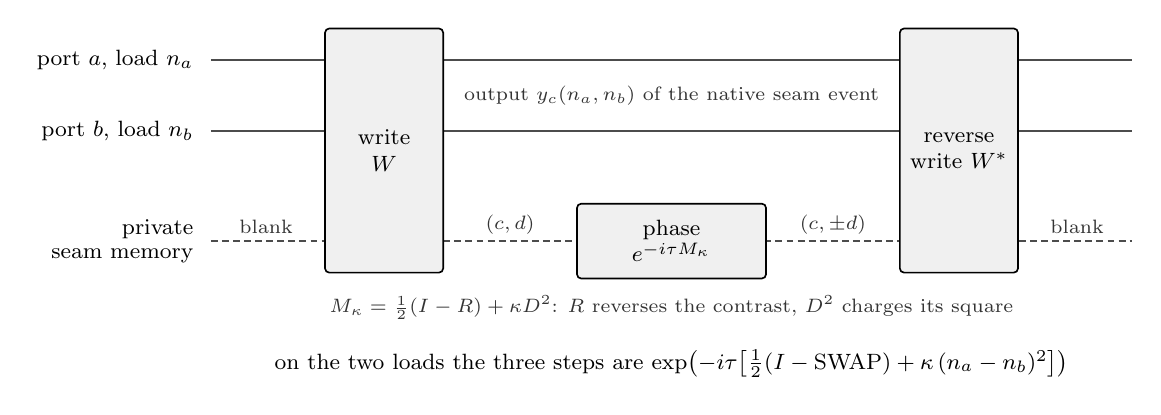
\begin{tikzpicture}[x=1cm,y=1cm,
  cms wire/.style={black!70, line width=0.6pt},
  cms mem/.style={black!70, line width=0.6pt, dash pattern=on 2.5pt off 1.5pt},
  cms gate/.style={draw=black, fill=black!6, rounded corners=1.5pt, line width=0.6pt,
    align=center, font=\footnotesize, inner sep=3pt},
  cms note/.style={font=\scriptsize, text=black!80, align=center, inner sep=1pt}]
% wires
\draw[cms wire] (0,1.7)--(11.7,1.7);
\draw[cms wire] (0,0.8)--(11.7,0.8);
\draw[cms mem] (0,-0.6)--(11.7,-0.6);
\node[anchor=east, font=\footnotesize] at (-0.1,1.7) {port $a$, load $n_a$};
\node[anchor=east, font=\footnotesize] at (-0.1,0.8) {port $b$, load $n_b$};
\node[anchor=east, font=\footnotesize, align=right] at (-0.1,-0.6) {private\\[-1pt]seam memory};
% gates
\node[cms gate, minimum width=1.5cm, minimum height=3.1cm] (W) at (2.2,0.55) {write\\$W$};
\node[cms gate, minimum width=2.4cm, minimum height=0.95cm] (Ph) at (5.85,-0.6)
  {phase\\$e^{-i\tau M_\kappa}$};
\node[cms gate, minimum width=1.5cm, minimum height=3.1cm] (Wd) at (9.5,0.55) {reverse\\write $W^{*}$};
% contents of the memory along the wire
\node[cms note, anchor=south] at (0.7,-0.55) {blank};
\node[cms note, anchor=south] at (3.8,-0.55) {$(c,d)$};
\node[cms note, anchor=south] at (7.9,-0.55) {$(c,\pm d)$};
\node[cms note, anchor=south] at (11.0,-0.55) {blank};
% contents of the ports between the two writes
\node[cms note, fill=white, inner sep=2pt] at (5.85,1.25) {output $y_c(n_a,n_b)$ of the native seam event};
\node[cms note, anchor=north] at (5.85,-1.25)
  {$M_\kappa=\tfrac12(I-R)+\kappa D^{2}$: $R$ reverses the contrast, $D^{2}$ charges its square};
\node[font=\footnotesize, anchor=north] at (5.85,-1.85)
  {on the two loads the three steps are
   $\exp\bigl(-i\tau\bigl[\tfrac12(I-\mathrm{SWAP})+\kappa\,(n_a-n_b)^{2}\bigr]\bigr)$};
\end{tikzpicture}

\caption{The echo on one seam. The write records the coin $c$ and the
contrast $d=n_a-n_b$ in the private memory and leaves the output of the
native seam event on the two ports. The phase acts on the memory alone.
The reverse write returns the memory to blank. On the loads the three steps
together are one event of the seam term of \eqref{eq:law}
(Theorem~\ref{thm:reduction}).}
\label{fig:echo}
\end{figure}

\begin{theorem}[Exact reduction]
\label{thm:reduction}
Let $J$ embed the loads of a seam into the blank memory,
$Jx=\ket{\blank}\otimes x$. For every real $\kappa$
\begin{equation}
h_\kappa J=J\Bigl[\frac{I-\SWAP}{2}+\kappa\,(n_a-n_b)^{2}\Bigr].
\label{eq:reduction}
\end{equation}
The local space is the orthogonal sum of three subspaces that $h_\kappa$
maps into themselves: the blank code $\ran J$, of dimension $9$, on which
$h_\kappa$ is the seam term \eqref{eq:reduction}; the written code $\ran W$,
of dimension $9$, on which $h_\kappa=0$; and the other records
$(\ran W)^{\perp}$ inside the record sector, of dimension $81$, on which
$h_\kappa=M_\kappa\otimes I$.
\end{theorem}

\begin{proof}
Two intertwining identities hold on every input:
\begin{equation}
(R\otimes I)\,W=W\,\SWAP,\qquad (D^{2}\otimes I)\,W=W\,(n_a-n_b)^{2}.
\label{eq:intertwine}
\end{equation}
The second holds because the label of $W\ket{a,b}$ carries $d=a-b$. For the
first, $(R\otimes I)W\ket{a,b}=2^{-1/2}\sum_c\ket{c,b-a}\otimes\ket{y_c(a,b)}$
and $W\ket{b,a}=2^{-1/2}\sum_c\ket{c,b-a}\otimes\ket{y_c(b,a)}$, and the
outputs agree by the symmetry of \eqref{eq:native}. Write
$h=\tfrac12(I-\SWAP)+\kappa(n_a-n_b)^{2}$. Then
$(M_\kappa\otimes I)W=Wh$, and
\[
h_\kappa Jx=U G_\kappa(0,Wx)=U(0,Whx)=\bigl(W^{*}Whx,\,(I-WW^{*})Whx\bigr)=(hx,0)=Jhx .
\]
For the second statement, $M_\kappa\otimes I$ is Hermitian and maps
$\ran W$ into itself, so it commutes with the projector $WW^{*}$. For
$z=Wx$ in the written code, $U(0,z)=(x,0)$ and $G_\kappa(x,0)=0$, so
$h_\kappa z=0$. For $z$ in the record sector with $W^{*}z=0$,
$U(0,z)=(0,z)$, $G_\kappa(0,z)=(0,(M_\kappa\otimes I)z)$ is again orthogonal
to $\ran W$, and $U$ fixes it. The three subspaces are orthogonal and their
dimensions add to $99$.
\end{proof}

The identities are polynomials of degree one in $\kappa$. Both coefficient
matrices were checked in exact arithmetic on all $99$ states, including the
inputs $(2,0)$, $(0,2)$, $(2,1)$, $(1,2)$ and $(2,2)$ and every memory state
that the echo never visits.

\begin{corollary}[Overlapping seams]
\label{cor:network}
Let $H_{\mathrm{joint}}$ be the sum of the local terms of all seams and of
the degree terms below, acting on all loads and all memories, and let
$J_{\mathrm{all}}$ embed the loads with every memory blank. Then
$H_{\mathrm{joint}}J_{\mathrm{all}}=J_{\mathrm{all}}H_\kappa$ and
$e^{-itH_{\mathrm{joint}}}J_{\mathrm{all}}=J_{\mathrm{all}}e^{-itH_\kappa}$
for every real $t$.
\end{corollary}

\begin{proof}
The term of a seam acts on the loads of its two ports and on its own
memory. On a vector of $\ran J_{\mathrm{all}}$ it acts by
\eqref{eq:reduction} and leaves every memory blank, although neighbouring
seams share a port and their terms do not commute. Summing over the seams
gives the first identity. $H_{\mathrm{joint}}$ is Hermitian and maps
$\ran J_{\mathrm{all}}$ into itself, which gives the second.
\end{proof}

The corollary concerns the sum of the local terms with a continuous
parameter. A finite program of echoes on seams that share ports is a
different object with its own schedule; Section~\ref{sec:events} treats it.
At $\kappa=0$ the echo is the exchange alone. That law is the control of
Section~\ref{sec:stability}.

\subsection{The degree term}

The seam terms alone give $\sum_e(n_a-n_b)^2=\sum_vd_vn_v^2-2\sum_en_an_b$,
which favours ports with five seams over ports with six: a pair on a seam
between two ports with six seams and two separate loads on ports with five
seams would have the same cost. A port with five seams therefore carries
one private reference register, a load system prepared in $\ket{0}$, with
an eleven-state memory of its own. On the port and its reference the law
uses the echo with the contrast part of the generator alone,
$U\bigl(0_{\blank}\oplus\kappa D^{2}\otimes I\bigr)U$. By
Theorem~\ref{thm:reduction} it reduces on the blank memory to
$\kappa(n_v-n_{\mathrm{ref}})^{2}$, which is diagonal, keeps the reference
at zero and equals $\kappa n_v^{2}$ there. The exchange part is left out on
this wire, because it would move load into the reference. Every port then
counts six, which gives the term $\sum_v(6-d_v)n_v^{2}$ of \eqref{eq:law}.

\subsection{What depends on the written output}

\begin{proposition}[Symmetry of the output]
\label{prop:symmetry}
Replace the native output in \eqref{eq:write} by any outputs $y'_c(a,b)$
that conserve the total. If $y'_c(a,b)=y'_c(b,a)$ for all inputs and both
coins, Lemma~\ref{lem:write} and Theorem~\ref{thm:reduction} hold with the
same right-hand side in \eqref{eq:reduction}.
\end{proposition}

\begin{proof}
The proofs used three properties of $W$: the isometry, which needs the
conservation of the total, and the two identities \eqref{eq:intertwine}.
The second identity uses the label alone, and the first is the stated
symmetry.
\end{proof}

The reduction was checked in exact arithmetic for four such replacements:
the sorted input with the coin ignored, the most concentrated pair of the
same total, the native output with the coin reversed, and one coin branch
used for both coins. All four give the seam term of \eqref{eq:reduction}.
A write that keeps the order of its inputs, $y'_c(a,b)=(a,b)$, violates the
first identity of \eqref{eq:intertwine}, and for it \eqref{eq:reduction}
fails. The equalization of the loads, the fair coin and the value of the
output therefore play no role in the induced law: the write is undone
exactly. The native seam event contributes its symmetry under exchange of
the two ports, and the binding of Section~\ref{sec:theorem} comes from the
supplied memory generator.


\section{The law on loads}
\label{sec:loads}

\subsection{Terms, costs and conserved quantities}

By Corollary~\ref{cor:network} the model with blank memories evolves the
loads by $H_\kappa=K+\kappa C$ of \eqref{eq:law}, with the exchange
$K=\tfrac12\sum_e(I-\SWAP_e)$ and the contrast cost $C$. Each
$\tfrac12(I-\SWAP_e)$ is a projector, so $K\ge0$. The term $\kappa C$ is
the agreement energy. In $C$ a load counts $6$, a doubled load counts $24$,
and every agreed seam takes $2$ off. For two loads this gives $C=10$ for a
pair on a seam, $C=12$ for two separate unit loads and $C=24$ for one
doubled load.

The exchanges permute the loads of the ports and $C$ is diagonal. The law
therefore conserves the number of loads $\sum_vn_v$ and the multiset of
loads, hence also $\sum_vn_v^{2}$. A doubled load stays doubled, and unit
loads on distinct ports stay unit loads on distinct ports. No event of the
law lowers the sum of the squared loads: the law is reversible and has no
settling. The sector of $N$ unit loads on $V$ ports has $\binom VN$ states.
The sector of two loads has $V(V+1)/2$ states, the $V(V-1)/2$ unit pairs and
the $V$ doubled loads, and the two parts do not mix.

\subsection{One load}

On one load $K$ is half the graph Laplacian $L$ of the carrier and $C=6$:
\begin{equation}
H_\kappa\big|_{\text{one load}}=\tfrac12L+6\kappa .
\label{eq:one-load}
\end{equation}
The agreement energy is a constant here, so the law of one load is the same
for every $\kappa$. On one cell the levels of $L/2$ are $0$ for the uniform
mode, $(5-\sqrt5)/2$ three times, $3$ five times and $(5+\sqrt5)/2$ three
times, the representations $1$, $3$, $5$ and $3'$ of the rotations. The
threefold level $(5-\sqrt5)/2$ is the slow band of the carrier paper: its
eigenspace is the range of the incidence Gram matrix of the twelve port
directions, which has rank three, and it is the slowest response of the
uniform repair mean \cite{ophmicro}. In the theory this rank-three response
is the material from which the observers' effective description with three
space dimensions is built \cite{ophspacetime}. The cell is no piece of
space. On the federation of $20$ cells the twenty lowest levels of one load
lie between $0$ and $0.17023$, one for each cell, and the next level is
$1.38197$.

\subsection{Loads \texorpdfstring{$0$ and $1$}{0 and 1}: the XXZ form}

On loads $0$ and $1$, with $n=(I-Z)/2$ and the Pauli matrices $X,Y,Z$ of
the two ports, the seam term of \eqref{eq:reduction} is
\begin{equation}
\frac{I-\SWAP}{2}+\kappa(n_a-n_b)^{2}
=\frac{(1+2\kappa)(I-Z_aZ_b)-X_aX_b-Y_aY_b}{4},
\label{eq:xxz}
\end{equation}
since $\SWAP=\tfrac12(I+X_aX_b+Y_aY_b+Z_aZ_b)$ and
$(n_a-n_b)^{2}=\tfrac12(I-Z_aZ_b)$. This is the ferromagnetic XXZ interaction
with anisotropy $\Delta=1+2\kappa$. Its bound clusters of overturned spins
are the droplet states of the XXZ chain \cite{nachtergaele2001} and of XXZ
systems on general graphs \cite{fischbacher2018}. Those results give the
context. The constants below are proved directly for this carrier and for
the complete sector of two loads with doubled loads.


\section{The binding theorem}
\label{sec:theorem}

\subsection{Ordered blocks}

\begin{lemma}[Ordered blocks]
\label{lem:blocks}
Let $H$ be Hermitian on a finite-dimensional space, $P$ an orthogonal
projector of rank $m$ and $Q=I-P$. Suppose
\[
PHP\le\mu_P\,P,\qquad QHQ\ge\mu_Q\,Q,\qquad\gamma=\mu_Q-\mu_P>0,\qquad
\lVert QHP\rVert\le\beta .
\]
Let $\lambda_1\le\lambda_2\le\dots$ be the eigenvalues of $H$. Then:
\begin{enumerate}[label=\textup{(\alph*)},leftmargin=2.2em,itemsep=1pt]
\item $\lambda_m\le\mu_P<\mu_Q\le\lambda_{m+1}$. Let $\Pi$ be the spectral
projector of $H$ on its $m$ lowest eigenvalues.
\item $\lVert Q\,\Pi\rVert\le\beta/\gamma$ and
$\lVert(I-\Pi)\,P\rVert\le\beta/\gamma$.
\item For every unit vector $\psi\in\ran P$ and every real $t$,
$\lVert Q\,e^{-itH}\psi\rVert\le2\beta/\gamma$.
\end{enumerate}
\end{lemma}

\begin{proof}
(a) By the min-max principle $\lambda_m$ is the least value, over subspaces
of dimension $m$, of the largest expectation of $H$ on the subspace. The
subspace $\ran P$ gives $\lambda_m\le\mu_P$. Also $\lambda_{m+1}$ is the
largest value, over subspaces of codimension $m$, of the least expectation
of $H$ on the subspace, and $\ran Q$ gives $\lambda_{m+1}\ge\mu_Q$. The
coupling between the blocks does not enter.

(b) Put $X=Q\Pi$, regarded as a map from $\ran\Pi$ to $\ran Q$, and let
$H_{\mathrm{low}}$ be the restriction of $H$ to $\ran\Pi$, with spectrum at
most $\mu_P$, and $H_Q=QHQ$ on $\ran Q$, with spectrum at least $\mu_Q$.
Since $\ran\Pi$ is invariant under $H$,
\[
XH_{\mathrm{low}}=QH\Pi=QH(P+Q)\Pi=(QHP)\,P\Pi+H_QX,
\]
so $H_QX-XH_{\mathrm{low}}=Y$ with $Y=-(QHP)\,P\Pi$ and
$\lVert Y\rVert\le\beta$. Put
$A=H_Q-\mu_P\ge\gamma$ and $B=H_{\mathrm{low}}-\mu_P\le0$. Then $AX-XB=Y$
and
\[
\frac{d}{ds}\Bigl(e^{-sA}Xe^{sB}\Bigr)=-e^{-sA}(AX-XB)e^{sB}=-e^{-sA}Ye^{sB}.
\]
Since $\lVert e^{-sA}\rVert\le e^{-s\gamma}$ and $\lVert e^{sB}\rVert\le1$
for $s\ge0$, integration from $0$ to $\infty$ gives
$X=\int_0^\infty e^{-sA}Ye^{sB}\,ds$ and
$\lVert X\rVert\le\lVert Y\rVert/\gamma\le\beta/\gamma$. This is the
Sylvester equation with ordered spectra \cite{bhatia1997}; the bound is the
one-sided form of the rotation estimates of Davis and Kahan
\cite{daviskahan1970}. For the second bound put $Z=(I-\Pi)P$, a map from
$\ran P$ to $\ran(I-\Pi)$, and let $H_{\mathrm{high}}$ be the restriction of
$H$ to $\ran(I-\Pi)$, with spectrum at least $\mu_Q$, and $H_P=PHP$ on
$\ran P$. Then
\[
H_{\mathrm{high}}Z-ZH_P=(I-\Pi)HP-(I-\Pi)PHP=(I-\Pi)\,(QHP),
\]
and the same argument gives $\lVert Z\rVert\le\beta/\gamma$.

(c) Split $\psi=\Pi\psi+(I-\Pi)\psi$. Both parts evolve inside their
spectral subspaces, so
\[
Q\,e^{-itH}\psi=Q\,\Pi\,e^{-itH}\Pi\psi+Q\,e^{-itH}(I-\Pi)P\psi ,
\]
and the two terms have norm at most $\beta/\gamma$ each by (b).
\end{proof}

The first term of (c) is the dressing of the band: the eigenvectors of the
lowest band are no pure vectors of $\ran P$. The second term is the part of
a state prepared in $\ran P$ that lies outside the band. Both are kept. The
weight outside the band, $\lVert(I-\Pi)e^{-itH}\psi\rVert^2\le\beta^2/\gamma^2$,
does not change with $t$. By convexity (c) holds for mixtures supported in
$\ran P$, and a preparation within norm distance $\epsilon$ of a unit
vector of $\ran P$ has
$\lVert Qe^{-itH}\psi\rVert\le2\beta/\gamma+\epsilon$. No spectral projector
is an operation of an observer; $\Pi$ appears in the proof alone.

\subsection{The theorem}

In the sector of two loads write $\ket{\{u,v\}}$ for unit loads on two
distinct ports $u,v$ and $\ket{2u}$ for a doubled load. Let $P$ project on
the span of the pairs on a seam, the states $\ket{\{a,b\}}$ with $\{a,b\}$ a
seam, and let $Q=I-P$. The range of $Q$ contains every separated pair and
every doubled load.

\begin{theorem}[Binding]
\label{thm:binding}
On every federation of complete cells whose external seams form a partial
matching on the ports, in the sector of two loads and for every
$\kappa\ge0$,
\begin{equation}
PH_\kappa P\le(10\kappa+6)\,P,\qquad
QH_\kappa Q\ge12\kappa\,Q,\qquad
\lVert QH_\kappa P\rVert\le\sqrt{10}.
\label{eq:blocks}
\end{equation}
For $\kappa>3$, every state $\rho$ supported in $\ran P$ and every real
value $t$ of the evolution parameter,
\begin{equation}
\Tr\bigl(Q\,e^{-itH_\kappa}\rho\,e^{itH_\kappa}\bigr)\le\frac{40}{(2\kappa-6)^{2}} .
\label{eq:binding}
\end{equation}
The constants do not depend on the number of cells or on the routing.
\end{theorem}

\begin{proof}
For a seam $e=\{a,b\}$ the projector $\tfrac12(I-\SWAP_e)$ annihilates a
basis state with $n_a=n_b$ and maps a basis state with $n_a\neq n_b$ to
half the difference of the state and its exchanged image. Hence, with
$[u\sim v]$ equal to one if $\{u,v\}$ is a seam and to zero otherwise,
\begin{align}
\bra{\{u,v\}}K\ket{\{u,v\}}&=\tfrac12(d_u+d_v)-[u\sim v], \label{eq:kdiag}\\
\bra{\{u',v\}}K\ket{\{u,v\}}&=-\tfrac12\quad\text{for }u'\sim u,\ u'\neq v, \label{eq:koff}
\end{align}
every other entry of $K$ between unit pairs vanishes, and $K$ maps unit
pairs to unit pairs and doubled loads to doubled loads.

\emph{The block of pairs.} A pair on a seam has $C=10$ and, by
\eqref{eq:kdiag} and Lemma~\ref{lem:incidence}(i), a diagonal entry of $K$
of at most $5$. By \eqref{eq:koff} two pairs on seams are joined by $K$
exactly when the moved load lands on a common neighbour of the two ends,
that is when the two seams are linked. So $PKP=T-\tfrac12M$ with a diagonal
matrix $T\le5$ and the adjacency matrix $M$ of the linked relation. By
Lemma~\ref{lem:incidence}(iv) $M$ is a direct sum over the cells of
matrices with no eigenvalue below $-2$ and of zeros on the external seams,
so $-\tfrac12M\le1$ and $PKP\le6$.

\emph{The complement.} On $\ran Q$ the cost $C$ is $12$ or $24$, and
$QKQ\ge0$ because $K\ge0$.

\emph{The coupling.} $C$ is diagonal, so $QH_\kappa P=QKP$. The column of a
pair on a seam $\{u,v\}$ has entries $-\tfrac12$ at the separated pairs
$\{u',v\}$ and $\{u,v'\}$, where $u'$ is a neighbour of $u$ other than $v$
that is no neighbour of $v$, and likewise for $v'$. Their number is
$d_u+d_v-2-2c$ with $c$ the number of common neighbours of $u$ and $v$. By
Lemma~\ref{lem:incidence}(ii) it is $d_u+d_v-6\le6$ for an internal seam and
$10$ for an external seam, so the absolute entries of a column sum to at
most $5$. The row of a separated pair $\{x,y\}$ has entries $-\tfrac12$ at
the pairs $\{w,y\}$ and $\{x,w\}$ with $w$ a common neighbour of $x$ and
$y$, so its absolute entries sum to the number of common neighbours, at
most $2$ by Lemma~\ref{lem:incidence}(iii). Rows of doubled loads vanish. A
matrix whose columns have absolute sums at most $5$ and whose rows have
absolute sums at most $2$ has norm at most $\sqrt{5\cdot2}$.

This proves \eqref{eq:blocks}. For $\kappa>3$ Lemma~\ref{lem:blocks}
applies with $\mu_P=10\kappa+6$, $\mu_Q=12\kappa$, $\gamma=2\kappa-6$ and
$\beta=\sqrt{10}$, and its part (c) with the remark on mixtures gives
\eqref{eq:binding}.
\end{proof}

\paragraph{The statement on records.}
The projectors on the pairs on the individual seams are mutually orthogonal
in the sector of two loads, and the complete seam reading of
Section~\ref{sec:reader} has one outcome for each seam and the outcome ``no
pair''. The left-hand side of \eqref{eq:binding} is the probability of ``no
pair''. A pair that starts on a seam is therefore read as a pair on some
seam with probability at least $1-40/(2\kappa-6)^2$ at every reading. The
value $t$ is audit. No translation invariance, preferred centre or global
observer enters the proof.

\paragraph{What the theorem leaves free.}
The bound concerns the two loads being read on one seam. It does not say on
which seam, and Section~\ref{sec:stability} shows that the pair is read on
other seams than the first. It does not require every configuration along
the evolution to be a pair on a seam. For a pair written on a seam
$\{a,b\}$ the probability of ``no pair'' is
$\tfrac14(d_a+d_b-2-2c)\,t^{2}$ to leading order in $t$, with $c$ as in
the proof: $t^{2}$ on one cell and $\tfrac54t^{2}$ on a seam whose ends
have six and five seams. In the sector of unit pairs the mean of $C$ is
$10$ plus twice that probability, so the agreement energy rises while the
pair dresses and the exchange compensates it; $H_\kappa$ is conserved. A
law of strict descent of $C$ would exclude this mechanism.

\subsection{Constants on the carriers}

The largest level of $PKP$ and the norm of $QKP$ were computed on the
carriers of Table~\ref{tab:carriers}; Table~\ref{tab:constants} compares
them with the bounds of the proof. With the computed constants, part (c) of
Lemma~\ref{lem:blocks} gives $17.3/(2\kappa-5.70)^{2}$ on the federations:
$0.163$ at $\kappa=8$ and $0.00028$ at $\kappa=128$, against $0.4$ and
$0.00064$ from \eqref{eq:binding}.

\begin{table}[!htb]
\centering
\caption{Constants of the binding theorem. The first column is the largest
level of the exchange on the pairs on seams, the second the largest
singular value of its coupling to the other states of two loads.}
\label{tab:constants}
\begin{tabular}{@{}lrr@{}}
\toprule
Carrier & Largest level of $PKP$ & $\lVert QKP\rVert$ \\
\midrule
one cell & $5.0000$ & $2.0000$ \\
$20$ cells & $5.7008$ & $2.0821$ \\
$80$ cells & $5.7000$ & $2.0811$ \\
$320$ cells & $5.7000$ & $2.0822$ \\
\midrule
every federation of the theorem & at most $6$ & at most $\sqrt{10}=3.1623$ \\
\bottomrule
\end{tabular}
\end{table}

\begin{proposition}[One cell]
\label{prop:cell}
On one cell, in the sector of two loads, the largest level of
$PH_\kappa P$ is $10\kappa+5$, the lowest level of $QH_\kappa Q$ is
$\min\bigl(12\kappa+4-\sqrt6,\ 24\kappa\bigr)$, and
$\lVert QH_\kappa P\rVert=2$. For $\kappa>(1+\sqrt6)/2$ a state supported in
$\ran P$ is read as ``no pair'' with probability at most
$16/(2\kappa-1-\sqrt6)^{2}$ at every reading.
\end{proposition}

\begin{proof}
Every port has five seams, so $PKP=4-\tfrac12M$ with $M$ the adjacency
matrix of the line graph of the dodecahedron. This graph has thirty
vertices and the incidence matrix $N$ of the dodecahedron has twenty rows,
so $N^{\mathsf T}N$ is singular and $-2$ is an eigenvalue of $M$: the
largest level of $PKP$ is $5$. The range of $Q$ is the sum of the separated
unit pairs, with $C=12$, and the doubled loads, with $C=24$, and $K$ does
not join the two. On the doubled loads $K$ is $L/2$ with lowest level $0$.
On the thirty pairs at distance two and the six antipodal pairs,
\eqref{eq:kdiag} gives the diagonal $5$; a load of a pair at distance two
moves to four separated positions at distance two and to two antipodal
positions, and a load of an antipodal pair moves to ten positions at
distance two. A vector equal to $x$ on the pairs at distance two and to $y$
on the antipodal pairs is an eigenvector with eigenvalue $\lambda$ when
$3x-y=\lambda x$ and $5y-5x=\lambda y$, that is
$\lambda^{2}-8\lambda+10=0$. The root $\lambda=4-\sqrt6$ has
$y=(\sqrt6-1)x$, an eigenvector with positive entries. The compression of
$K$ to the separated pairs has no positive entries off the diagonal, so its
lowest eigenvector can be chosen with nonnegative entries and cannot be
orthogonal to a positive one: $4-\sqrt6$ is the lowest level. Each column
of $QKP$ has four entries $-\tfrac12$, each row of a pair at distance two
has four and each antipodal row none, so $\lVert QKP\rVert\le2$, and the
uniform vector on the thirty pairs on seams attains $2$. The last statement
is Lemma~\ref{lem:blocks} with $\gamma=2\kappa-1-\sqrt6$ and $\beta=2$; for
these $\kappa$ the first term of the minimum is the smaller one.
\end{proof}

At $\kappa=8$ the bound of Proposition~\ref{prop:cell} is $0.102$ and at
$\kappa=128$ it is $0.00025$.


\section{Emitter, reader and agreed records}
\label{sec:instruments}

\subsection{The local emitter}

The emitter at a seam $e=\{a,b\}$ is one fuel state $\ket{F}$ that carries
the resource of two loads and is coupled to the pair $\ket{e}=\ket{\{a,b\}}$
on that seam. Its energy is the diagonal entry of the law at the pair,
\begin{equation}
E_F=10\kappa+\tfrac12(d_a+d_b-2),\qquad
H_{\mathrm{emit}}=H_\kappa+E_F\proj{F}+g\bigl(\ket{F}\bra{e}+\ket{e}\bra{F}\bigr),
\label{eq:emitter}
\end{equation}
and the coupling $g$ acts for the duration $\pi/(2g)$ while the law acts
throughout. No eigenvector of the law is installed, and fuel left in the
emitter is an outcome of every later reading.

\begin{proposition}[Emitter]
\label{prop:emitter}
Let $\psi$ be the state after the pulse from the initial state $\ket{F}$.
Then
\[
\bigl\lVert\psi+i\,e^{-iE_F\pi/(2g)}\ket{e}\bigr\rVert\le\frac{\sqrt{d_a+d_b-2}}{2g} .
\]
\end{proposition}

\begin{proof}
Let $r=(H_\kappa-E_F)\ket{e}$. By \eqref{eq:kdiag} and \eqref{eq:koff} it is
the sum of $-\tfrac12$ times the $d_a+d_b-2$ distinct states reached from
the pair by one exchange, so $\lVert r\rVert^{2}=(d_a+d_b-2)/4$, and $r$ is
orthogonal to $\ket{e}$ and $\ket{F}$. Put
$H_{\mathrm{emit}}=H_{0}+\ket{r}\bra{e}+\ket{e}\bra{r}$. Under $H_0$ the
states $\ket{F}$ and $\ket{e}$ have the same energy $E_F$ and are coupled
to each other alone, so
$\psi_0(s)=e^{-iE_Fs}\bigl(\cos(gs)\ket{F}-i\sin(gs)\ket{e}\bigr)$ and
$\psi_0(\pi/2g)=-i\,e^{-iE_F\pi/(2g)}\ket{e}$. By Duhamel's formula
\[
\psi-\psi_0(\tfrac{\pi}{2g})=-i\int_0^{\pi/(2g)}e^{-i(\pi/(2g)-s)H_{\mathrm{emit}}}
\bigl(\ket{r}\bra{e}+\ket{e}\bra{r}\bigr)\psi_0(s)\,ds ,
\]
and the integrand has norm $\lvert\sin(gs)\rvert\,\lVert r\rVert$. The
integral of $\lvert\sin(gs)\rvert$ over the pulse is $1/g$.
\end{proof}

\begin{corollary}
\label{cor:emitted}
On a federation as in Theorem~\ref{thm:binding} with $\kappa>3$, at every
reading after the pulse the probability of the outcomes ``no pair on a
seam, a doubled load, or fuel'' is at most
\[
\Bigl[\frac{2\sqrt{10}}{2\kappa-6}+\frac{\sqrt{d_a+d_b-2}}{2g}\Bigr]^{2}
\le\Bigl[\frac{2\sqrt{10}}{2\kappa-6}+\frac{\sqrt{10}}{2g}\Bigr]^{2}.
\]
At $\kappa=128$ and $g=64$ the right-hand side is
$64009/25600000=0.0025003515625$ on every seam of every such federation.
\end{corollary}

\begin{proof}
After the pulse the coupling is off and the evolution preserves the norm
distance of Proposition~\ref{prop:emitter}. The remark after
Lemma~\ref{lem:blocks} applies with that distance as $\epsilon$, and
$d_a+d_b\le12$.
\end{proof}

With the same constants the weight outside the band of pairs or in the fuel
is at most $(\sqrt{10}/250+\sqrt{10}/128)^{2}=35721/25600000$, constant
after the pulse. The duration and the coupling of the pulse, the fuel and
the switch are resources of the apparatus. Errors of timing or
initialization add to these bounds.

\subsection{The reader and the complete outcome set}
\label{sec:reader}

At a seam $e=\{a,b\}$ the predicate
\[
b_e=\mathbf 1\{n_a=n_b=1\},
\]
``both ends hold one load'', is read at both ends. The reader of a seam has
eleven bits: a value bit and a validity bit for the pointer at each of the
two ports and for a courier, two decision bits, and three public record
bits. It acts in four stages. The pointer at the first port receives a copy
of $b_e$ and is set valid. The pointer at the second port does the same.
The courier copies the first pointer and carries it to the second port. The
comparator then writes the decision: \emph{agreement} if the second pointer
and the courier are both valid and hold the same value, \emph{mismatch} if
both are valid and differ, \emph{unavailable} if one of them is invalid; a
reader that has not run is \emph{pending}. On agreement,
and then alone, the comparator writes the agreed value into the three
public bits. An \emph{agreed record} of the seam is the public value one
with the decision agreement.

Each stage is an exclusive-or gate and therefore a permutation of all
$2^{11}$ words of the reader that is its own inverse; the reader is
reversible on every input, clean or not. The four stages were composed and
inverted on all $2^{11}$ words for both values of $b_e$ and for four
variants: the nominal reader, a courier that flips the message (decision
mismatch), a second pointer that is never written (decision unavailable)
and both pointers holding the wrong value. The last variant ends in agreement
on a wrong value. Agreement by itself does not prove that a reading was
correct; it is the condition under which a record is admitted. After
admission the public record has no generator of its own. It is a supplied
protected memory, and its three copies give no protection against a common
corruption of all three.

In the sector of two loads the predicates of different seams exclude each
other, so the complete reading of all seams has one outcome for each seam
and one further outcome, ``no pair''. On the federation of $20$ cells these
are $630$ records and ``no pair''. Separated loads, doubled loads and fuel
left in the emitter all fall under ``no pair''. Their separate weights are
audit of the computation and no information that the readers of the seams
hold.

The seam memory of the law stays private and unread. Seam records are
committed at the reading. Every reported reading uses a fresh run, and a
reading is never used to hold the object in place: after an ideal complete
reading the loads are in the mixture
$\rho\mapsto\sum_eP_e\rho P_e+Q\rho Q$ with $P_e$ the projector on the pair
on the seam $e$, which is a different state from the unread one.

\subsection{Interference and Bell correlations in the observer records}

A single sharp load at port zero evolves for one exchange time with
every contact open. Admit the amplitudes at two neighbouring apertures,
ports 5 and 7, and release them for a second unit. The return detector
at port zero clicks on $5.684\%$ of all simulated launches with both
apertures open at zero relative phase. Opening each alone gives a sum
of $2.899\%$. Reading the aperture and forgetting its value gives
$2.845\%$. A relative phase of $\pi$ gives $0.013\%$. Absorption is
included in each denominator. With no aperture inserted, uninterrupted
flight gives $11.666\%$ return, against $13.712\%$ with an unread
midpoint position measurement.

Two initially sharp loads at ports 1 and 3 of the same cell evolve
under the free two-load generator on all 630 seams of the 20-cell
board. At exposure eight two other cells isolate a local seam each.
Each observer reads whether its seam has absolute contrast one and
undoes the echo. This flags exactly one arrival and preserves coherence
between the two port addresses. The receiver seams and exposure were
selected by a survey of 870 seam pairs at four times. Nine independent
local calibration settings determine the two analyzer axes for each
observer. Both capture flags precede independently sampled settings.
Each local analyzer uses a degree phase, a blank-seam rotation and an
echo that records positive, negative or quiet. The analyzer operations
commute and each marginal law is independent of the distant setting.

Fresh simulated counts give 533,643 joint captures in $2^{28}$ launches.
On these event-ready trials the Clauser--Horne--Shimony--Holt score
is $2.7005$, with a simultaneous 99\% lower bound of $2.6604$ from
the four correlation estimates. The Bell-local bound under independent
settings is 2 \cite{chsh1969}. Giving every quiet reading the fixed score $+1$ yields
$1.6311$ across all launches. Reading which port was occupied before the
analyzer reduces the capture score to $-0.0536$. Exchange alone gives
$1.2368$ with the same apparatus. At exposures $7.5$ and $8.5$, the
fixed axes give capture scores of $0.6301$ and $2.1934$. With two
addressed half contacts and full-swap routing to cells five steps apart,
a different preparation gives $2.4143$ across all launches, in agreement
with $1+\sqrt2$.

Two independent sources on a five-owner route can also swap
entanglement. Each source begins with sharp loads and prepares a pair
using controlled contacts and a fresh seam write. The middle owner
receives one encoded load from each source and records the two
commuting Bell parities. The outer owners then choose their settings
locally, before either receives the middle record. Joining the records
after the measurements fixes the sign convention for each parity.
All four middle outcomes and every launch contribute. In $2^{22}$
simulated trials per menu the sign-corrected CHSH estimate is $2.8282$
with simultaneous 99\% lower bound $2.8084$. The exact ideal value is
$2\sqrt{2}$. On a separate menu the independent-source witness
$\sqrt{|I|}+\sqrt{|J|}$ is $1.4144$, with lower bound $1.4074$ against
the bilocal bound of one \cite{branciard2012}. Here $I$ averages the four outer correlations
with the middle $ZZ$ parity, and $J$ uses the $XX$ parity and reverses
the sign for unequal settings. Reading the two alternatives of one
source before flight removes both violations. Each required local number
phase can be synthesized with ten timed native contacts and two empty
guard ports. Replaying this implementation reproduces all twelve
archived count arrays. The preparation schedule,
controlled routing, independently initialized setting coins and Born
readout specify the apparatus. The experiment identifies correlations
in its simulated terminal records. Establishing physical spacelike
separation requires independently calibrated times and ranges.

The probability premise admits a separate finite material test. On a
connected blank register with one accessible private reference,
addressed native contacts generate independent special-unitary
control in each fixed load inventory. The private squared-load phase
separates the three possible species exchanges. Further diagonal
phases at spectator ports distinguish the individual exchanges
between material configurations. Commuting these generators along a
connected path gives all off-diagonal matrix units of each block.
This construction supplies operations for a common public event in
several readers. In a six-address register two branches represent
the same effect $H$. Separate readers measure $H$ and $2H$.
For $2{,}932{,}736$ simulated launches of the same prepared mixture
per reader, the first two branches return $733{,}955$ and $732{,}421$,
the independent $H$ reader returns $732{,}852$, and the $2H$ reader
returns $1{,}468{,}130$. A transverse cubic rule consistent with the
earlier finite menu predicts probabilities $143/512$ and $35/64$.
These records distinguish that rule from the specified quantum
instrument. On a rotated mixture, readings along three axes reconstruct
a state with lower eigenvalue at least $0.37441$. It predicts a held
union of two noncommuting coexistent effects at $0.550278$. The
common and separate readers give $0.550067$ and $0.549558$.
Extending the probability argument to all public records
requires the operational readout premises on those records.

What happens when the material publishes a record during flight?
Halfway to the same appointment, the two source gateways write their
signed contrasts. A local pointer keeps each result after the inverse
echo restores the material. All contacts then act for the remaining
four units. Pooling all nine pairs of midpoint signs yields 427,481
joint captures and a score of $0.7467$ at the original settings.
Nine new axis measurements select new settings, which give $0.9800$
on fresh captures. If $T$ is the two-qubit correlation matrix on
these pooled captures, the maximum score over rotations of the two
local projective meters is $2\sqrt{s_1(T)^2+s_2(T)^2}$, where $s_1,s_2$
are its largest singular values. Simultaneous counting bounds on the
nine entries give an upper bound of $1.011$ at 99\% coverage. Which
records the cells publish during the flight determines whether these
observers can detect a violation.

The free evolution starts from a product configuration. Coherent native
evolution and the declared Born instrument supply the joint outcome
law. A capture record conditions the history before the analyzer
settings are drawn. The blank-seam experiment does not derive this law
from committed classical records. Local isolation implements
the operational separation of the two wings. A spacelike
interpretation requires a corresponding physical clock and range test.

\subsection{Reading while the law acts}

A reading of finite duration is performed with the law acting. Stage $j$ of
the reader of a seam $e$ is the involution $S_{e,j}$ and has the generator
\[
\Lambda_{e,j}=\frac{\pi}{2\tau_j}\bigl(I-S_{e,j}\bigr),\qquad
e^{-i\tau_j\Lambda_{e,j}}=S_{e,j},
\]
because $\tfrac12(I-S_{e,j})$ projects on the eigenvalue $-1$ of $S_{e,j}$.
During stage $j$ the complete generator is
$H_\kappa+\sum_e\Lambda_{e,j}$ together with the energy of the fuel; the
reading lasts $\tau_{\mathrm{read}}=\sum_j\tau_j$.

\begin{proposition}[Reader with the law acting]
\label{prop:reader}
In the sector of two loads of a carrier whose ports have at most $d$ seams,
let $U_{\mathrm{act}}$ be the complete evolution over the reading of any
set of seams and $U_{\mathrm{ref}}$ the same evolution with the exchange
$K$ removed. Then $U_{\mathrm{ref}}$ is the ideal reading at the start of
the reading followed by a phase that is diagonal in the loads, and
\[
\lVert U_{\mathrm{act}}-U_{\mathrm{ref}}\rVert\le2d\,\tau_{\mathrm{read}} .
\]
The distribution of the complete public records differs from that of the
ideal reading at the start by at most $2d\,\tau_{\mathrm{read}}$ in total
variation, for every $\kappa$ and every number of seams read at once.
\end{proposition}

\begin{proof}
The stage generators are controlled by the diagonal predicates $b_e$ and
act on distinct registers. They commute with each other, with $\kappa C$
and with the energy of the fuel. Without $K$ the evolution of stage $j$ is
therefore the product of the $S_{e,j}$ and of a diagonal phase, and the
phases can be collected after the stages. Duhamel's formula gives
$\lVert U_{\mathrm{act}}-U_{\mathrm{ref}}\rVert\le\lVert K\rVert\,\tau_{\mathrm{read}}$.
By \eqref{eq:kdiag} a diagonal entry of $K$ is at most $d$ on a unit pair,
and it is at most $d/2$ on a doubled load. In both cases the absolute
entries off the diagonal in the same row sum to the diagonal entry, so
$\lVert K\rVert\le2d$. For unit vectors the trace distance of
the two outputs, and with it the total variation distance of any complete
measurement, is at most the norm distance.
\end{proof}

On the federations $d=6$, and for $\tau_{\mathrm{read}}=1/16384$ the bound
is $3/4096=0.000732421875$. The comparison is with the ideal reading at the
start of the reading; the proposition does not claim that the two pointers
copy an unchanged load.

One such reading was executed with every state kept: the reader of one seam
of one cell, on the emitted state at $\kappa=128$ and $g=64$ after an
evolution of four units, with four stages of duration $1/65536$ each. The
joint space of the $78$ states of two loads, the fuel and the $2^{11}$
reader words has dimension $161{,}792$. The state differs from the
reference by $2.44\times10^{-4}$ in norm, against the bound
$10\,\tau_{\mathrm{read}}=6.10\times10^{-4}$ of the cell, and the public
records by $2.09\times10^{-7}$ in total variation. The agreed record of the
seam has probability $0.19502961$, against $0.19502982$ for the ideal
reading; this is the probability for one seam at one reading and no
probability that a pair is read somewhere. The decisions have weight
$1.2\times10^{-10}$ on mismatch and $4.7\times10^{-11}$ on unavailable.

\subsection{Error budget}

Table~\ref{tab:budget} collects the bounds for the emitter at $\kappa=128$
and $g=64$ and a complete reading of duration $1/16384$ on any federation
of Theorem~\ref{thm:binding}. After one complete reading every admitted
branch is a pair on a seam, to which the theorem applies again, and the
outcome ``no pair'' keeps its weight; the last line follows. Further
readings need fresh records and add their own errors. No error-free
unlimited observation is claimed.

\begin{table}[!htb]
\centering
\caption{Bounds on the probability of every outcome other than an agreed
record of a pair, at $\kappa=128$, $g=64$ and
$\tau_{\mathrm{read}}=1/16384$, on every federation of
Theorem~\ref{thm:binding}.}
\label{tab:budget}
\begin{tabular}{@{}L{8.2cm}ll@{}}
\toprule
Step & Added & Bound \\
\midrule
emitter and free evolution, ideal reading & & $0.0025003515625$ \\
reading with the law acting & $3/4096$ & $0.0032327734375$ \\
free evolution after one complete reading, ideal second reading & $0.00064$ & $0.0038727734375$ \\
\bottomrule
\end{tabular}
\end{table}


\section{Events and clocks}
\label{sec:events}

\subsection{The law as local events}

One event is one seam acting once with an angle $\tau$. As the echo
\eqref{eq:echo-event} on blank memories it acts on the loads as
$\exp\bigl(-i\tau\bigl[\tfrac12(I-\SWAP_e)+\kappa(n_a-n_b)^2\bigr]\bigr)$.
Since $(n_a-n_b)^2=n_a^2+n_b^2-2n_an_b$ and $n_a^2+n_b^2$ commutes with the
exchange of the seam, this is the product of
\begin{equation}
E_e(\tau)=\exp\Bigl(-i\tau\Bigl[\frac{I-\SWAP_e}{2}-2\kappa\,n_an_b\Bigr]\Bigr)
\label{eq:event}
\end{equation}
and of the phase $\exp\bigl(-i\tau\kappa(n_a^2+n_b^2)\bigr)$ of the two
ports on their own loads. In the law with a continuous parameter the port
phases of all seams and the degree term add to $6\kappa\sum_vn_v^2$, which
the law conserves, and they change no record. In a finite program the phase
of a port does not commute with the events of its other seams, so the two
forms are different programs. The programs of this section use the event
\eqref{eq:event}, the seam term without its port part, and need no
reference registers. In the memory it is the echo whose phase reads the
product of the two loads from the recorded contrast $d$ and the total $s$
of the written output, $n_an_b=\tfrac14(s^2-d^2)$; the reduction of
Theorem~\ref{thm:reduction} holds for it on all $99$ states, with
$-2\kappa n_an_b$ in place of $\kappa(n_a-n_b)^2$.

A program is a sequence of events. A port takes part in the events of its
own seams and counts them, and that count is a local clock of its observer.
No common count is assumed. The position of an event in the sequence is
audit.

\begin{proposition}[Each port's own order]
\label{prop:order}
Two programs in which every port sees the events of its seams in the same
order give the same state, and therefore the same probabilities of all
records.
\end{proposition}

\begin{proof}
Events on two seams without a common port act on different loads and
memories and commute. Let $e$ be the first event of the first program. In
the second program no event on a seam that shares a port with $e$ can come
before the first occurrence of $e$, since the shared port would see a
different first event. That occurrence can therefore be
commuted to the front. Removing it from both programs leaves two programs
with the same property, and induction on the length finishes the proof.
\end{proof}

No order between events on seams that share no port enters a record.
The statement was also executed: a program of $3{,}000$ events and a
second one obtained from it by $12{,}141$ exchanges of neighbouring events
without a common port give the same seam records on one cell, with largest
difference $0$, and $19{,}722$ exchanges on $20$ cells give a largest
difference of $1.1\times10^{-41}$.

\subsection{Schedules}

Table~\ref{tab:programs} reports four kinds of program at $\kappa=8$,
started from a pair on one seam. In a round every seam acts once, in an
order drawn afresh for each round. In the rounds with two rates the seams
between ports of one half of the carrier act twice in every round. In the
last two programs every event draws its seam at random, with equal weights
or with double weight on that half. The readings are the seam records after
every thirty events on one cell and after every $630$ events on $20$ cells;
the total angle per seam is $32$ on one cell and $8$ on $20$ cells.

\begin{table}[!htb]
\centering
\caption{The law as local events at $\kappa=8$: largest probability of ``no
pair'' over all readings along the program, and the range of the ports'
own counts at the end of the programs with angle $1/64$.}
\label{tab:programs}
\begin{tabular}{@{}L{4.5cm}rrrL{5.0cm}@{}}
\toprule
Program & One cell, & One cell, & $20$ cells, & Ports' own counts \\
 & $\tau=1/64$ & $\tau=1/256$ & $\tau=1/64$ & (one cell; $20$ cells) \\
\midrule
rounds, every seam once & $0.0217$ & $0.0137$ & $0.0188$ & all $10240$; $2560$ to $3072$ \\
rounds, one half twice & $0.0470$ & & $0.0268$ & $10240$ to $16384$; $2560$ to $6144$ \\
random seam, equal rates & $0.5048$ & $0.1897$ & $0.1989$ & $10063$ to $10428$; $2419$ to $3184$ \\
random seam, two rates & $0.5206$ & $0.1522$ & $0.2859$ & $8170$ to $13366$; $1616$ to $4275$ \\
\bottomrule
\end{tabular}
\end{table}

Rounds keep the pair, with equal and with unequal rates. The ports' own
counts then differ by a factor of up to $2.6$, and no common count exists.
Seams that act independently at random lose the pair at these angles. The
loss falls with the angle: on one cell the largest probability of ``no
pair'' is $0.505$ at $\tau=1/64$, $0.190$ and $0.184$ for two programs at
$1/256$, and $0.085$ at $1/1024$, a factor $2.2$ for a factor $4$ in the
angle.

Seams without a common port can act in parallel. One cell has five classes
of six such seams, and on a federation the same five classes hold in every
cell and the external seams form a sixth. One symmetric period applies all
classes except the last for half the angle, the last for the full angle,
and the others in reverse order for half the angle, a splitting of second
order \cite{strang1968}. Its error against the law with a continuous
parameter falls with the square of the angle: at $\kappa=2$ the state of a
pair differs in norm by $0.337$, $0.0215$ and $0.00134$ at angles $1/8$,
$1/32$ and $1/128$ on one cell after a total angle $16$, and by $0.0916$
and $0.00578$ at $1/8$ and $1/32$ on $20$ cells after a total angle $4$.
No closed constant for this error is claimed. On records at $\kappa=8$, for a
pair started on one seam, the layered program gives a probability of ``no
pair'' of $0.0064$ on one cell after a total angle $32$ at angle $1/256$,
in both orders of the classes, which is the value of the continuous law,
and of $0.0076$ and $0.0075$ in the two orders on $20$ cells after a total
angle $8$ at angle $1/64$, against $0.0076$.

\subsection{What the binding rests on}

Two members of the memory family differ in what an event leaves behind. In
the law the memory is unread and returns to blank. In the committed member
the contrast of the acting seam, which of its ends holds a load, is
committed to a public record after every event. On one cell at $\kappa=8$
with rounds of angle $1/64$ the committed member does not hold the pair:
the probability of ``no pair'' is $0.015$, $0.11$ and $0.32$ after $64$,
$512$ and $2048$ rounds, while the unread member has a largest value of
$0.018$ over all readings. Records of the port loads written during the
evolution at a rate $\gamma$ per port act in the same direction. On one
cell, from the lowest level of two unit loads, the probability of a pair on
a seam at parameter values $0$, $128$, $256$, $384$, $512$ is $0.859$,
$0.865$, $0.869$, $0.870$, $0.869$ at $\kappa=2$ and $\gamma=0.001$, and
$0.859$, $0.844$, $0.778$, $0.717$, $0.666$ at $\gamma=0.01$; at
$\kappa=4$ and $\gamma=0.01$ it is $0.951$, $0.941$, $0.915$, $0.889$,
$0.863$. A uniformly random pair has $0.455$.

The binding rests on the regular phase between successive events of a
seam. A port that serves each of its seams once per round supplies that
regularity with its own count and needs no other clock. Independent
random service and records committed at every event disturb it. The
theorems of Section~\ref{sec:theorem} are proved for the law with a
continuous parameter, the limit of small angle, and the results of
Section~\ref{sec:stability} are stated for that law.


\section{Particle stability}
\label{sec:stability}

\subsection{The claim on records}

Particle stability is an observable that the seam interaction reproduces,
under the reference candidate and in the free sector of Interval Echo,
which uses it at $\kappa=8$. The claim is about agreed seam records.

\emph{Observers and records.} The two ends of every seam report one agreed
record, ``both ends loaded''. The complete set of outcomes is
one record for each seam and the outcome ``no pair''; fuel left in the
emitter counts as ``no pair''.

\emph{Claim.} A pair of loads written on one seam by a local emitter is read
as a pair on some seam with probability at least one minus the bound,
whenever the observers read. It is read on other seams than the first.
Nothing holds it except the law. Under the same law without the agreement
energy the record is lost.

\emph{Clock.} The claim uses none. The bound holds at every value of the
evolution parameter, hence at every reading in any observer's own history.
The sampled values of the parameter below are audit.

\emph{What counts against the claim.} ``No pair'' above the bound at a
reading; no level of two loads below the energy of two free loads, an
audit on the spectrum; or a changed law with the same alphabet, routing and
symmetry that gives the same answer on the whole property.

The words ``the pair moves'' mean ``the pair is read on other seams''. A
seam is a place in the carrier, which is hardware of the computation, and
the statement is no statement about a position in physical space.

\subsection{Readings}

The emitter of Section~\ref{sec:instruments} with $g=64$ writes a pair on
an internal seam; on the federations one end of that seam carries an
external seam. The law then acts, and the seam records are read at the
parameter values $0,4,\dots,32$, each in a fresh run.
Table~\ref{tab:stability} and Figure~\ref{fig:stability} give the largest
probabilities over these readings. The bound is that of
Lemma~\ref{lem:blocks} with the constants of the carrier from
Table~\ref{tab:constants} and the emitter's error,
$\bigl[2\beta/(2\kappa-\mu)+\sqrt{d_a+d_b-2}/(2g)\bigr]^{2}$, with $\mu$
the largest level of $PKP$ and $\beta=\lVert QKP\rVert$.

\begin{table}[!htb]
\centering
\caption{Particle stability on agreed seam records. The probabilities are
the largest values over the readings of each run.}
\label{tab:stability}
\begin{tabular}{@{}lrrrr@{}}
\toprule
Carrier & $\kappa$ & Bound & Largest $P$(no pair) & Largest $P$(pair on another seam) \\
\midrule
one cell & $8$ & $0.148790$ & $0.00956834$ & $0.985996$ \\
one cell & $128$ & $0.001447$ & $0.00001881$ & $0.991270$ \\
$20$ cells & $8$ & $0.182975$ & $0.00962164$ & $0.977029$ \\
$20$ cells & $128$ & $0.001606$ & $0.00002270$ & $0.933194$ \\
$80$ cells & $8$ & $0.182787$ & $0.00964389$ & $0.977130$ \\
$80$ cells & $128$ & $0.001605$ & $0.00002270$ & $0.933194$ \\
$320$ cells & $8$ & $0.182965$ & $0.00963435$ & $0.977091$ \\
\bottomrule
\end{tabular}
\end{table}

\begin{figure}[!htb]
\centering
% Figure: particle stability of the contrast-memory seam, the law of the reference candidate
% A-contrast-memory-spherical-v1; the main candidate law, Interval Echo, uses the same seam at kappa = 8.
% Largest probability of the outcome "no pair" over the readings of each run, against the bounds, on a
% logarithmic axis.
% Horizontal position of a probability p: 2 (log10 p + 5) cm, that is 2 cm per decade from p = 10^-5.
% The positions below are computed from the probabilities given in the trailing comments.
\begin{tikzpicture}[x=1cm,y=0.88cm,
  cms read/.style={circle, fill=black, draw=black, inner sep=0pt, minimum size=2.1mm},
  cms bound/.style={rectangle, fill=white, draw=black, line width=0.6pt, inner sep=0pt, minimum size=2.1mm},
  cms control/.style={diamond, fill=black!45, draw=black, line width=0.5pt, inner sep=0pt, minimum size=2.7mm}]
% grid and axis
\foreach \k/\lab in {0/10^{-5},1/10^{-4},2/10^{-3},3/10^{-2},4/10^{-1},5/1}
  {\draw[black!18, line width=0.4pt] (2*\k,0.15)--(2*\k,-5.05);
   \node[font=\scriptsize, anchor=north] at (2*\k,-5.1) {$\lab$};}
\draw[black!70, line width=0.5pt] (0,-5.05)--(10,-5.05);
\node[font=\footnotesize, anchor=north] at (5,-5.55) {probability of the outcome ``no pair''};
% one run: label, height, position of the computed value, of the bound with carrier constants, of the uniform bound
\def\CMSrun#1#2#3#4#5{%
  \node[font=\footnotesize, anchor=east] at (-0.25,#2) {#1};
  \draw[black!45, line width=0.5pt] (#3,#2)--(#4,#2);
  \draw[black, line width=0.9pt] (#5,#2-0.14)--(#5,#2+0.14);
  \node[cms bound] at (#4,#2) {};
  \node[cms read] at (#3,#2) {};}
\CMSrun{one cell, $\kappa=8$}{-0.15}{5.9617}{8.3451}{9.2707}% 0.00956834, 0.14879, 0.431861
\CMSrun{$20$ cells, $\kappa=8$}{-0.65}{5.9665}{8.5248}{9.2707}% 0.00962164, 0.182975, 0.431861
\CMSrun{$80$ cells, $\kappa=8$}{-1.15}{5.9685}{8.5239}{9.2707}% 0.00964389, 0.182787, 0.431861
\CMSrun{$320$ cells, $\kappa=8$}{-1.65}{5.9676}{8.5247}{9.2707}% 0.00963435, 0.182965, 0.431861
\CMSrun{one cell, $\kappa=128$}{-2.3}{0.5488}{4.3209}{4.7960}% 1.881e-05, 0.001447, 0.00250035
\CMSrun{$20$ cells, $\kappa=128$}{-2.8}{0.7121}{4.4115}{4.7960}% 2.27e-05, 0.001606, 0.00250035
\CMSrun{$80$ cells, $\kappa=128$}{-3.3}{0.7121}{4.4110}{4.7960}% 2.27e-05, 0.001605, 0.00250035
% changed laws on 20 cells
\node[font=\footnotesize, anchor=east] at (-0.25,-3.95) {$20$ cells, exchange alone};
\node[cms control] at (9.8027,-3.95) {};% 0.796828
\node[font=\footnotesize, anchor=east] at (-0.25,-4.45) {$20$ cells, energy reversed};
\node[cms control] at (6.1840,-4.45) {};% 0.012359
% legend, in the empty upper left part of the plot
\node[draw=black!40, fill=white, line width=0.4pt, inner sep=3pt, anchor=north west] at (0.2,0.05) {%
\scriptsize
\begin{tabular}{@{}c@{\hspace{5pt}}l@{}}
\tikz[baseline=-0.6ex]{\node[cms read] {};} & largest value read\\
\tikz[baseline=-0.6ex]{\node[cms bound] {};} & bound, constants of the carrier\\
\tikz[baseline=-0.6ex]{\draw[black, line width=0.9pt] (0,-0.12)--(0,0.12);} & bound, every federation\\
\tikz[baseline=-0.6ex]{\node[cms control] {};} & changed law, largest value read
\end{tabular}};
\end{tikzpicture}

\caption{The largest probability of ``no pair'' over the readings of each
run of Table~\ref{tab:stability}, on a logarithmic axis, with the bound for
the constants of the carrier and the bound of Corollary~\ref{cor:emitted}
for every federation. The two lowest lines are the changed laws of
Table~\ref{tab:controls}, which have no bound of this kind.}
\label{fig:stability}
\end{figure}

The readings lie a factor of $15$ to $77$ below the bounds and do not
change with the number of cells. At long parameter values on $20$ cells
and $\kappa=8$ the probability of ``no pair'' is $0.0089$, $0.0088$ and
$0.0084$ at $64$, $256$ and $1024$, and the probability of a pair on
another seam than the first is $0.676$, $0.926$ and $0.977$.

\emph{Single readings.} On $20$ cells at $\kappa=8$ the reading at
parameter value $32$ returns ``no pair'' with probability $0.007660$. Of
$100{,}000$ sampled single readings $786$ return ``no pair'', the pair is
read on $59$ different seams, and $1{,}538$ readings find it on the first
seam, where the probability is $0.01531$.

\emph{Audit on the spectrum.} Count energies from $12\kappa$, the energy of
two free loads in the uniform mode. The lowest level of two loads lies at
$-14.07$ on $20$ cells and at $-14.24$ on one cell, and it is a pair on a
seam with probability $0.987$ and $0.986$. The pair is bound by the law and
by no trap: the level lies below the energy at which two loads are free. At
$\kappa=0.5$, $1$ and $2$ on $20$ cells the lowest level lies at $-0.355$,
$-1.002$ and $-2.596$ and is a pair on a seam with probability $0.570$,
$0.712$ and $0.861$.

\subsection{Controls}

\emph{Changed laws.} Table~\ref{tab:controls} repeats the run on $20$ cells
for two laws with the same alphabet, routing and symmetry. The exchange law
alone, $\kappa=0$, loses the pair. Its lowest level of two unit loads is
the uniform state at $0$, in which a pair on a seam has the probability
$630/28680=0.022$ of a uniformly random pair. With the agreement energy
reversed, $-\kappa$ in place of $\kappa$, the pair is kept in free
evolution. Lemma~\ref{lem:blocks} explains this: free persistence follows
from the isolation of the band of pairs, and with the reversed sign the
pairs form the highest band. What the sign of the law adds is the level
below two free loads. With the reversed sign every level of two unit loads
lies above $0$ and the lowest holds no pair. The property of the claim is
persistence together with binding, and both changed laws give another
answer on it.

\begin{table}[!htb]
\centering
\caption{Changed laws on $20$ cells with $\kappa=8$. The lowest level is
that of two unit loads, counted from the energy of two free loads.}
\label{tab:controls}
\begin{tabular}{@{}lrrr@{}}
\toprule
Law & Largest $P$(no pair) & Lowest level & Pair on a seam in it \\
\midrule
the law & $0.0096$ & $-14.07$ & $0.987$ \\
exchange alone, $\kappa=0$ & $0.7968$ & $0$ & $0.022$ \\
agreement energy reversed & $0.0124$ & $+0.0066$ & $0.00002$ \\
\bottomrule
\end{tabular}
\end{table}

\emph{A state without the property.} Two loads on ports of different cells,
under the law, are read as an agreed pair with probability at most
$0.00004$ at $\kappa=8$ over the same readings.

\emph{Planted laws.} Three planted changes test the reader and count for
nothing else. Without any exchange the pair stays on its seam, with a
probability of $0$ on another seam, and the case is excluded because
nothing is read elsewhere. One loss channel from the first seam raises the
largest probability of ``no pair'' from $0.0096$ to $0.038$. With the
agreement energy removed on the thirty seams of the emitter's cell the
reader shows $0.81$.

\emph{Changes of the test.} The four checks of the claim (the pair is kept
within the bound, it is read on other seams, a level lies below two free
loads, the control loses the pair) were also run under six deliberate
changes of the law, the emitter and the control, on one cell and on $20$
cells. The law passes the four checks, and each check fails under at least
one change.

\subsection{The face object}

Three loads on the three ports of one face form the face object
(Figure~\ref{fig:cell}). Its record is the conjunction of the agreed
records of the three seams of a face. Started on one face at $\kappa=8$ and
read at the same parameter values, the outcome ``no agreed face'' has
probability at most $0.0178$ on one cell and $0.0174$ on $20$ cells, and
the object is read on another face with probability up to $0.980$ and
$0.944$. Under the exchange law alone ``no agreed face'' reaches $0.80$ on
one cell and $0.97$ on $20$ cells. The sectors of three unit loads have
$220$ and $2{,}275{,}280$ states.

The colour read can be applied to the same three loads after binding.
Leave every internal contact of the source cell open and shutter its
external contacts. Prepare three sharp loads on a face. A finite
spectrometer admits $19.95\%$ of launches near the bound energy
$100.448$ in exchange units, below the one-load plus two-load threshold
of $129.764$. A coarse face measurement preserves coherence between
faces. Route three local groups of ports into separately calibrated
colour triplets, using the supplied coherent change of basis for each
group. After 32 free units, 32,525 of 524,288 original launches pass
the face, three-triplet and antisymmetric-singlet tests; another 39,483
pass the first two and fail the last. The singlet fraction of these
three-triplet records is $45.2\%$. The normalized antisymmetric state
has three equal Schmidt coefficients across each one-versus-two cut.
Every biseparable three-triplet state consequently has singlet fidelity
at most $1/3$. The counts resolve genuine tripartite entanglement in the
decoded state. A common noncentral colour turn gives a resolved dark-port signal,
excluding pure singlet behaviour
for this source and decoder. The colour frames are fitted, and each
occupied tip carries one ordinary material unit.

A different three-body test uses one period-three density wall on each
of three connected ten-port belts. A three-load wall has material
polarization $-1/3$ and a four-load wall $+2/3$, relative to the
prepared periodic background. The comparison places a compact cluster
on each belt with both bridge endpoints empty. Its mean energy, after
subtracting the common sector constant, is $-167$ for ten loads and
$-199$ for eleven. Let $P$ record one such wall on each belt.
The exchange generator is positive, and the interaction counts $-16$
per doubly occupied seam. At most three or four such seams occur on
these wall words, respectively. The norm of the coupling out of $P$ is
bounded by $\sqrt{102}/2$ or $\sqrt{108}/2$ by counting incoming and
outgoing exchanges. For any state supported in energy at or below the
comparison value, the two gaps of 119 and 135 give wall probabilities
at most $0.181\%$ and $0.149\%$. This constrains low-energy composites
on the gated guide, including coherent superpositions of all configurations.
The comparison gives no bound on a composite in an upper band.

\paragraph{Flux response of a moving density wall.}
On a ten-port belt a probe can give each microscopic hop of signed
length $d$ an external phase $d\Phi/10$. A circuit by one ordinary
unit fixes the sign and normalization. Translating a sharp wall three
sites carries one unit one site backwards or two sites forwards, giving
material charges $-1/3$ and $+2/3$. Calibrate the dispersion at zero
flux and compare the same source released under opposite twists.
On twelve held combinations of twist and momentum per wall, the maximum
errors of the rigid fractional-charge forecasts are $0.01596$ and
$0.01373$ exchange units. The best integer alternatives miss by
$0.37831$ and $0.33070$. Both fractional forecasts exceed the
prespecified tolerance of $0.01$. The full exchange permits temporary
excursions out of the sharp-wall configurations. A Schur complement accounts for motion through the other
configurations and bounds the dominant
splittings at 24 further settings within intervals narrower than $10^{-6}$.
The measured phase slopes lie within $0.00035$ of those intervals.
The probe couples to material transport by design. Independent native
probes covering both poles resolve an integral total load, including
on compact, nonwinding preparations of the same load. Identifying an
electric charge requires a field measurement that distinguishes these
preparations. With a stationary interferometer in an adjacent cell,
the three-load wall gives phases of $-0.02279$ and $+0.01086$ radians
on oppositely signed probes. The corresponding single-unit calibrations
are $+0.09274$ and $+0.01103$. Blocking material exchange between the
belt and the intervening gateway removes both wall signals.

\paragraph{A singlet selected by the source energy.}
A second preparation uses the three equivalent gateway arms of the
home cell. Keep the full contact energies at the boundary while
preventing outward hops during the preparation. One sharp face has
overlap with a simple line at $100.8894585$ native energy units.
The guarded generator commutes with the permutations of the three
arms. The line transforms by their sign. Within the admitted tensor
product of three equivalent triplet readers its image is therefore
the unique antisymmetric determinant. Energy selection alone prepares
the line. The filter admits $8.3645\%$ of original starts.
Applying a calibrated half-turn to all three readers gave zero dark
outcomes in $36{,}525$ admissions. Turning one reader alone gave
$15{,}517$ dark outcomes in $36{,}871$ admissions.

After full release on $20$, $80$ and $320$ cells, the conditional
probability that the three loads remain connected exceeds $98.34\%$
at every time. One exchange time after release the singlet fraction
among admitted triplets exceeds $99.92\%$ on every board. On $20$
cells at least $34{,}742$ of $2^{30}$ original starts can be assigned
to the singlet under the certified simulation error. The complete
denominator includes source and orbital refusals. The arm permutation
is a spatial symmetry of the guarded source. Identifying the observed
triplet action as the physical colour charge of three quarks requires
an independent matter and gauge measurement. One such check times a
full period of the native material-number phase on each constituent.
The three readouts gave $36{,}326$, $36{,}858$ and $36{,}717$ bright
outcomes, respectively, with zero dark. A coupling of $+2/3$ or
$-1/3$ of the ordinary load unit would give $75\%$ dark. An orbital
colour-centre rotation on one receiver gives that dark fraction.
These two rotation instruments distinguish the orbital colour phase
from fractional charge under the native number service.

\paragraph{Three local observers test a common colour rotation.}
On the protected energy-selected trimer, each observer reads one orbital
label in each of four common qutrit basis settings on separate cohorts.
The sum over bases of the equal-label effects for a pair is its identity
plus its swap. Summing over pairs gives a positive operator with spectrum
$0,3,6$ whose kernel is the determinant line. A count of pair coincidences
thus bounds its weight for every mixed three-qutrit preparation.
After a shared remote rotation the conditional singlet fidelity exceeds
$0.99974$ at simultaneous $99\%$ confidence. The four cohorts admitted
$585{,}045$ of $17{,}179{,}869{,}184$ simulated launches. Reversing
the order on the other two arms gives an upper bound of $0.89748$,
and measuring and forgetting the original labels gives $0.50877$.
An independent single-load inverse-word calibration predicts the ordered
three-label tables. A shared clock measures conjugate centre phases on
one arm and on the complementary pair, with unit return on all three.
These tests use supplied orbital frames and local Born instruments.

After one free exchange unit, the local position test can also measure
connectivity and orbital colour on the same released excitation. All six
words of the determinant in the main aperture occupy a connected triple.
At simultaneous $99\%$ confidence the connected-singlet fraction among
admissions exceeds $0.99561$, $0.99776$ and $0.99774$ on 20, 80 and
320 cells, corresponding to 32--37 per million original launches. Each
aperture and board had four cohorts totalling $2^{34}$ simulated launches.
In two alternative apertures the determinant words are all disconnected.
Both gave orbital singlet fidelity above $0.9825$ on 20 cells but exactly
zero connected-singlet weight. Dephasing or mismatching the rotations
reduced the main upper fidelity bounds to $0.62917$ and $0.91438$.

A separate ten-port belt tests the proposed identification of period-three
wall winding with transported material charge. On the sharp four-load
cycle three revolutions carry two ordinary units. A calibrated cut counter
in free evolution instead recorded $630{,}665$ returns to the same word
with odd transport in $2^{30}$ original launches at time 16. A change of
boundary phase also separates a spectral line of the isolated native
band by more than $0.00856$ in exchange units. The sharp-cycle counter
predicts zero odd returns and identical phase spectra. An electric charge
assignment requires a response of the moving wall to a separately
calibrated electric field.

\paragraph{Separating a triplet and an antitriplet.}
Place one locally decoded colour triplet in each of three cells, with
two adjacent triplets in the antisymmetric antitriplet. On the
320-cell federation a seam-parity and occupation read at contact gives
a connected mean energy of $-0.17696\pm0.00015$ for the selected
octet and $-0.00001\pm0.00005$ for the singlet. Beyond contact the
connected operator vanishes on all nine admitted colour states,
through 22 cell steps. A separate prepared material domain costs
17 exchange units per cell. Its two outer wall records also occur
in configurations of cost 34 at every tested separation of at least
two cells when interior walls are allowed. Linear growth on this guide
measures the work of preparing the entire domain. A confining force
would require the colour sources themselves to sustain a separation
energy after the intervening matter relaxes. On 80 cells a fourth load ranges
freely over 924 ports outside the three occupied source cells. Relative
to the stronger isolated source, its additional singlet binding falls
from $0.10937$ exchange units at two steps to $0.00305$ at four.
At ten steps the calculated binding is below $10^{-6}$, and the
phase measurement gives a ground-energy shift of
$-0.00056\pm0.00034$. A mobile load therefore mediates a short-range
attraction on these placements.

\paragraph{What forces a string between two recorded endpoints?}
On three federations, compare the loads at each exterior bridge and
record the parity of the mismatches around each face. A mismatch is
an edge of the dual graph. With two odd faces and even parity on
every other face, the mismatch edges must contain a path connecting
the two sources. Each unit of length costs at least 32 native energy
units on the active exterior bridges, and a shortest path with symmetric
bridge states attains $32d$ at face distance $d$. If only the two
source parities are fixed, each can pair locally with another odd face.
The exact minimum becomes $32\min(d,2)$. On 320 owners the phase
meter gives $352.005$ at separation eleven under the full parity
constraint and $64.002$ with screening allowed. The corresponding
sharp, inventory-guarded preparations cost $32.5$ per mismatch. Both exterior
comparisons park the internal seams and private reference services.
With every contact and service active, the sector of blank memories,
vacancies and double loads at half filling admits a separate variational
bound. A number-preserving permutation touching at most 48 ports,
followed by projection onto the two odd readings, gives an admissible
trial state of bounded excess energy over the unconstrained ground,
uniformly in separation. The conservative upper bound of $19{,}129$
native units permits a finite linear window.

A distinct result applies to hard endpoint families related by
transposing two owners, including their internal memories.
The transposition changes at most six exterior seam expectations
by at most 33 each and six private reference costs by at most 32
each. The variational principle bounds the difference between the
two relaxed energies by 390 for arbitrary occupancy. For two bounded
additive sources on one state family the absolute connected ground
work is bounded by the smaller source's spectral width. The results
distinguish a global constraint that sustains tension from the work
of two local pins. Linking a conserved sector to physical colour and
determining its tension in physical units remain open.

\subsection{Unequal seams}

With every seam term multiplied by a strength $1+\delta_e$,
$\lvert\delta_e\rvert\le w$, drawn independently, one draw for each $w$,
the lowest level of two
unit loads on $20$ cells at $\kappa=2$ stays below the energy of two free
loads and stays a pair: $-2.596$ with a pair on a seam at probability
$0.861$ for $w=0$, $-2.668$ with $0.868$ for $w=0.1$, and $-2.796$ with
$0.879$ for $w=0.2$. The binding uses no symmetry between the seams.


\section{What a reading leaves}
\label{sec:presence}

The reader of Section~\ref{sec:instruments} keeps one record for every seam.
A second instrument keeps one answer for the whole cell, and the two leave
different states behind.

\subsection{The presence reading}

On one cell with the fuel, let $P_e$ be the projector on the pair on the
seam $e$, $P=\sum_eP_e$ the projector on the thirty pairs on seams, and
$Q=I-P$ the projector on the other $49$ states. The presence reading runs
the four stages of the reader on every seam, combines the thirty public
words by a tree of reversible OR gates of depth five, copies the root into
a fresh public register, and runs the tree and the readers backwards
(Figure~\ref{fig:run}). Every
gate is an involution on its register. The scratch registers return to
blank for every basis state of the loads, and by linearity for every state.
Orthogonal record labels are copied and nothing else. One read allocates
$720$ bits. With one switch set, the public word of every seam is copied
into an archive of its own before the reversal, which gives the reader with
seam records in the same circuit.

For a state $X$ of the loads, a positive answer acts as
\begin{equation}
X\longmapsto PXP
\qquad\text{and}\qquad
X\longmapsto\sum_eP_eXP_e
\label{eq:presence}
\end{equation}
for the presence reading and for the reader with seam records, and a
negative answer acts as $X\mapsto QXQ$ for both. Both find a pair with the
same probability. The presence reading leaves the pair spread over the
seams as it was. The reader with seam records places it on one seam. A
state supported on one answer block is left unchanged by the presence
reading. On the uniform superposition of the thirty pairs the two positive
outputs differ by $29/30$ in trace distance, the largest value over all
inputs.

\begin{figure}[!htb]
\centering
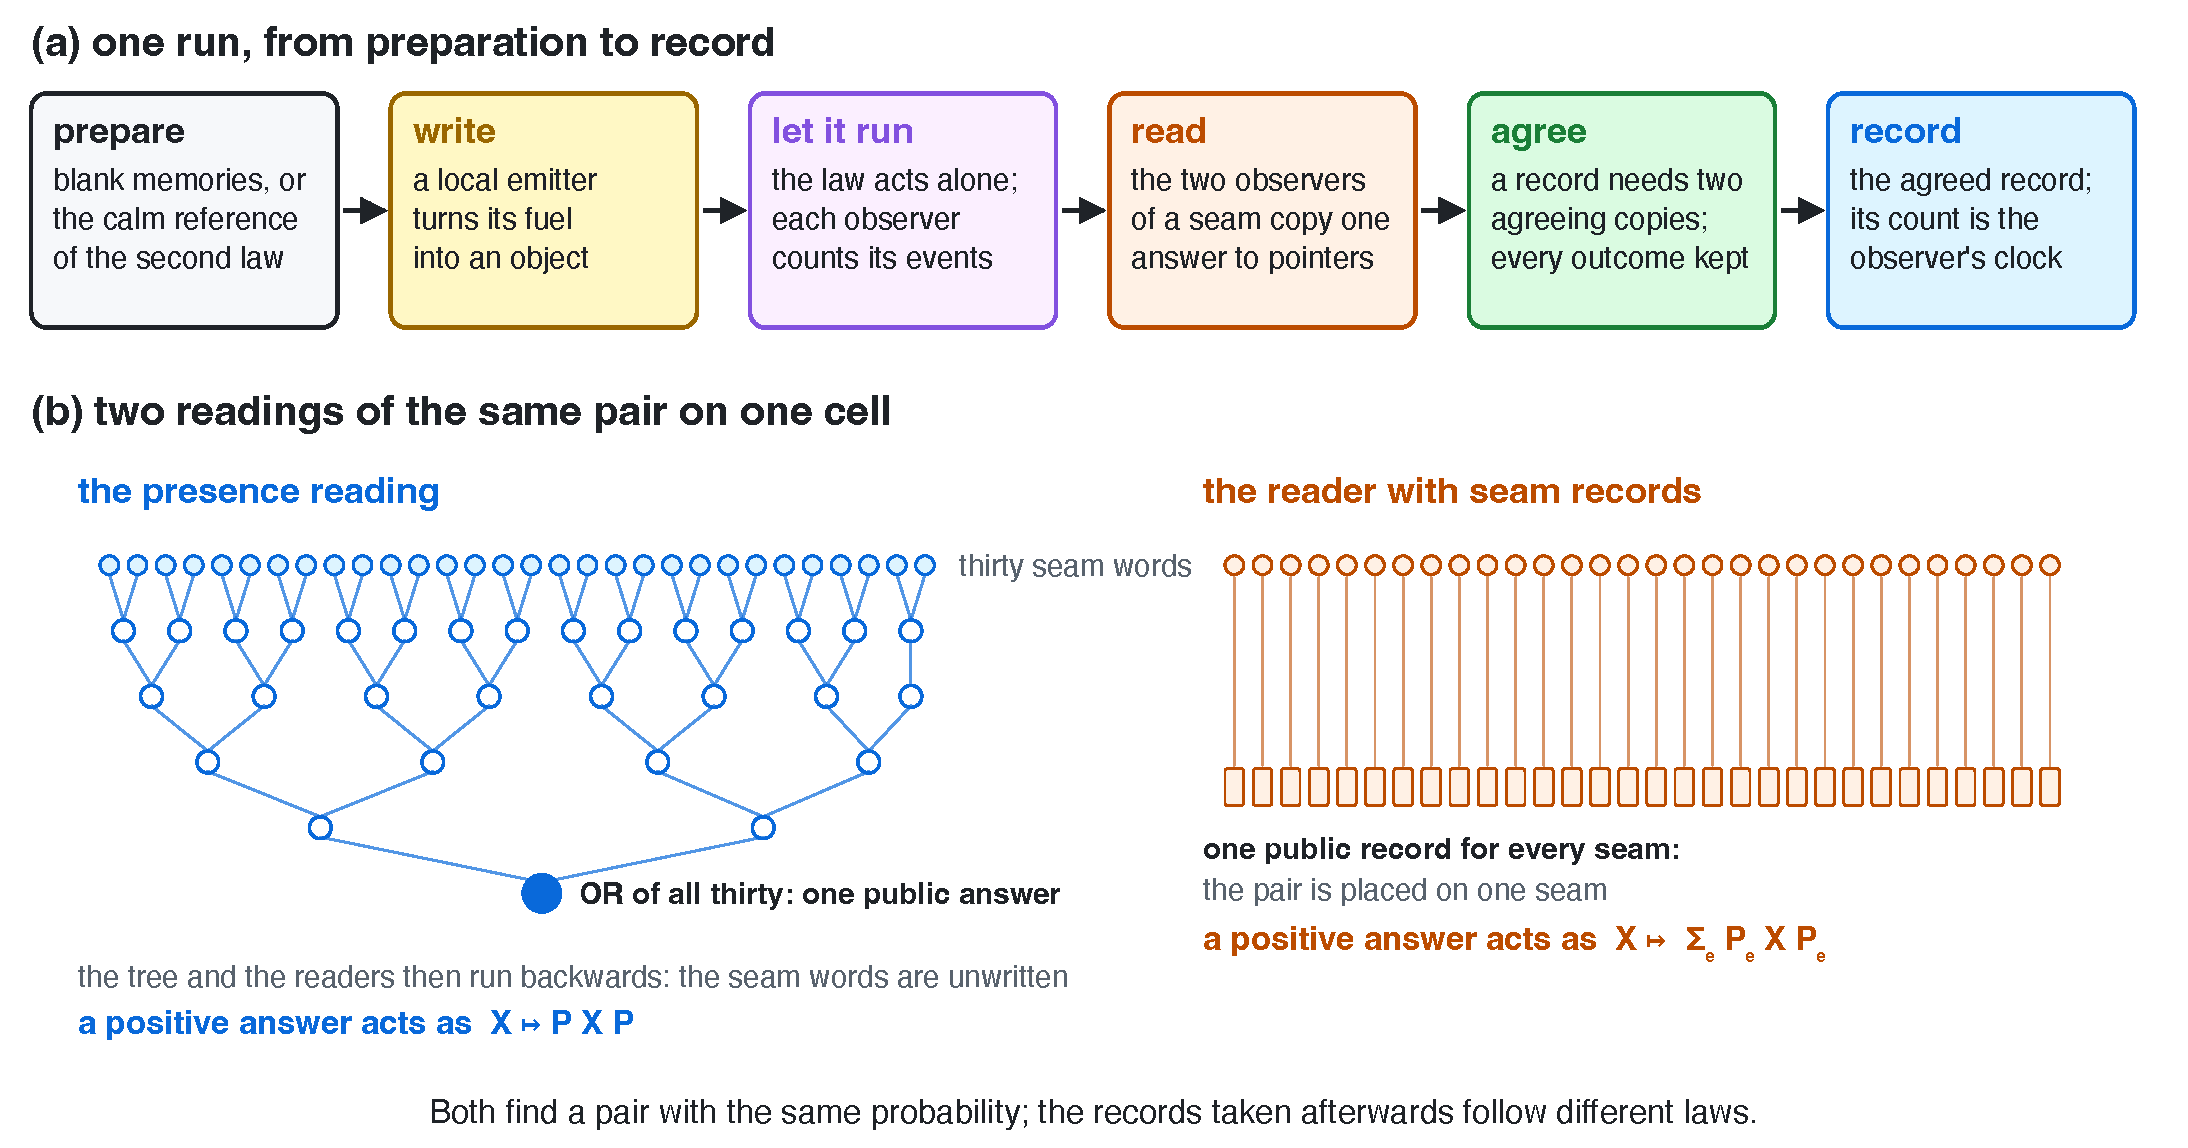
\includegraphics[width=\linewidth]{figures/model_run.pdf}
\caption{Observers, instruments and records. (a) One run, the same for the
reference candidate and the scalar channel: a preparation, a local write by
an emitter, the law acting alone while
every observer counts its own events, a reading copied into two pointers,
agreement of the two copies, and the agreed record whose count is the
observer's clock. (b) The presence reading combines the thirty seam words by
a reversible tree, copies one answer and unwrites the words; the reader with
seam records keeps thirty records. Table~\ref{tab:presence} gives the laws
of the later records.}
\label{fig:run}
\end{figure}

\subsection{Two readings in one history}

The emitter writes the pair on the seam $(0,1)$ of one cell at
$\kappa=8$ and $g=64$. After four units of the exchange the observers take
a first reading, the presence reading or the reader with seam records.
After four further units they take a final reading with seam records. The
seam of the first reading is hidden in both histories before they are
compared, so that both show the same public alphabet: one first answer and
one final record. The first answer has the same law in both histories. The
laws of the complete histories differ (Table~\ref{tab:presence}).

\begin{table}[!htb]
\centering
\caption{Two readings of a pair on one cell: the probability of a positive
first answer, equal for both instruments, and the total variation between
the laws of the two public histories.}
\label{tab:presence}
\begin{tabular}{@{}L{7.6cm}rr@{}}
\toprule
Run & First answer positive & Total variation \\
\midrule
contrast-memory law, $\kappa=8$ & $0.992329$ & $0.440513$ \\
exchange alone, $\kappa=0$ & $0.647174$ & $0.196148$ \\
contrast of the reversed sign, $\kappa=-8$ & $0.987884$ & $0.249676$ \\
$\kappa=8$, reports of the first seam mismatch or are not available & $0.747346$ & $0.260336$ \\
$\kappa=8$, every predicate flipped in agreement & $1$ & $0.446650$ \\
\bottomrule
\end{tabular}
\end{table}

These numbers take a reading as instant, with the diagonal part of the law
acting during its window. With the exchange acting through both read
windows of length $w=1/16384$, the law of one experiment differs from this
calculation by at most $24w$ in total variation, and a comparison of two
experiments by at most $48w$. One event is certified in exact arithmetic
with every such error counted: a positive first answer followed by a final
record on the emitting seam has the probabilities $0.0182640$ under the
presence reading and $0.1029264$ under the reader with seam records, and
the total variation between the two public histories exceeds $0.0817$.

The pair of Section~\ref{sec:stability} is one object spread over seams.
An instrument that asks where it is places it, and later records show the
difference. The event of the binding theorem, a pair on some seam, has an
instrument of its own that measures that event and nothing more.


\subsection{What finite return counts certify on Interval Echo}
\label{sec:four-return-readings}

A mobile excess has twelve enrolled addresses arranged in six pairs.
A fixed distant vacancy balances the preparation. Four stations each
read one material bit at two appointments. Serial comparison of the first
word publishes the pair. The bitwise exclusive-or of the second word and
the first gives the returned address. For each pair we prepare its two individual
addresses and their two equal superpositions of opposite sign, then use
the matching analyzer before the terminal read. A valid return requires
both the correct first label and the expected terminal bit. Every launch,
including an unavailable or malformed report, enters the denominator.

Write $F_Z,F_X$ for the mean return probabilities in the two bases on a
single pair. The calibrated first reader has the exact pair projector as
its effect. Its restricted channel therefore preserves trace, including
all output addresses. For the normalized Choi matrix $J$, the matching
projectors in the two bases share the maximally entangled vector $\Phi$.
Their remaining directions on the pair are orthogonal Bell vectors.
Thus $\langle\Phi|J|\Phi\rangle\geq F_Z+F_X-1=f$, the
complementary-basis bound of Hofmann~\cite{hofmannreturns}. The trace
distance of $J$ from $\Phi$ is at most $\sqrt{1-f}$. Preparing an
arbitrary correlated input by filtering the reference half of $\Phi$
multiplies this bound by at most two. Hence any unconditioned subsequent public event on the public label,
outgoing data and untouched reference
differs in probability from the ideal pair reading by at most
$\min(1,2\sqrt{1-f})$ when $0\leq f\leq1$. Each first operation is
supported on its own input projector. Weighting the six conditional
bounds by the first probabilities therefore covers every input on the
enrolled code. The compiled writers preserve that code. The four-bit
decoder can alias an empty data cell to address zero outside it.

Twenty-four fresh calibration settings returned $8{,}192$ correct
outcomes each. Exact one-sided binomial limits with simultaneous error
allocation give $f\geq0.9979316$ on each pair. The measured bound on any
later event is $0.0910$. A comparison writer records the low address bit
and then forgets it. It publishes the same first label but its observed
error on the negative-sign probe exceeds $0.4813$ on each pair. At two
held phases the ideal bright probabilities are $(2\pm\sqrt2)/4$.
The pair reader gave $0.84863$--$0.85926$ and $0.14245$--$0.14954$ on
the six pairs. The comparison writer gave $0.48583$--$0.50806$.
The guarantees have joint confidence $99\%$ for independent launches of
the specified stable devices. These are simulated pointer records with
calibrated preparations and terminal analyzers. The companion code gives
the counts for $491{,}520$ fresh launches and the event-bound proof.

\section{Bound objects}
\label{sec:objects}

\subsection{Costs}

An object is a set of $N$ unit loads. Its cost in $C$ is
\begin{equation}
C=6N-2\,(\text{number of agreed seams}).
\label{eq:cost}
\end{equation}
Table~\ref{tab:objects} lists, for each $N$ on one cell, the objects with
the most agreed seams. The first three belong to the three kinds of centre
of the cell, its $12$ ports, $30$ seams and $20$ faces, the $62$ points in
which the rotation axes meet the cell. The last column is the least amount
by which the cheapest object of $N$ loads undercuts two cheapest objects of
$k$ and $N-k$ loads. It is at least $2$ throughout: at strong coupling no
object gains by falling apart. No object is protected against merging. The
cost per load falls from $6$ to $1$, and the whole cell costs $12$, the
same as one face. What protects an object in this law is the conserved
number of loads and the gap of the law. The law holds no winding and no
flux.

\begin{table}[!htb]
\centering
\caption{The cheapest objects of $N$ unit loads on one cell. The last
column is the least gain over the splits into two parts.}
\label{tab:objects}
\small
\begin{tabular}{@{}rlrrrr@{}}
\toprule
$N$ & Shape & How many & Agreed seams & Cost & Gain against a split \\
\midrule
$1$ & one port & $12$ & $0$ & $6$ & \\
$2$ & one seam & $30$ & $1$ & $10$ & $2$ \\
$3$ & one face & $20$ & $3$ & $12$ & $4$ \\
$4$ & two faces on a seam & $30$ & $5$ & $14$ & $4$ \\
$5$ & three faces round a port & $60$ & $7$ & $16$ & $4$ \\
$6$ & a port and its five neighbours & $12$ & $10$ & $16$ & $6$ \\
$7$ & that cap and one more port & $60$ & $12$ & $18$ & $4$ \\
$8$ & the cell less a face and a port & $30$ & $15$ & $18$ & $6$ \\
$9$ & the cell less a face & $20$ & $18$ & $18$ & $6$ \\
$10$ & the cell less a seam & $30$ & $21$ & $18$ & $6$ \\
$11$ & the cell less a port & $12$ & $25$ & $16$ & $8$ \\
$12$ & the whole cell & $1$ & $30$ & $12$ & $10$ \\
\bottomrule
\end{tabular}
\end{table}

\subsection{Bindings at finite coupling}

At finite $\kappa$ the lowest level $E_N$ of $N$ unit loads on one cell is
a single state, invariant under the rotations of the cell.
Table~\ref{tab:bindings} gives its binding $B_N=6\kappa N-E_N$ against $N$
free loads in the uniform mode. These are levels of the law in units of the
exchange and audit on the spectrum. The bindings follow the numbers of
agreed seams $1$, $3$, $5$, $7$, $10$ of Table~\ref{tab:objects}: at
$\kappa=8$ the lowest levels hold $0.986$, $2.985$, $4.986$, $6.989$ and
$9.995$ agreed seams on average. The binding of the pair lies between $0$
and one sixth of the cost $12\kappa$ of its two loads. In the lowest level
of the pair on one cell a pair on a seam has probability $0.60$, $0.72$,
$0.86$, $0.99$ and $1.00$ at $\kappa=0.5$, $1$, $2$, $8$ and $128$.

\begin{table}[!htb]
\centering
\caption{Binding $B_N$ of the lowest level of $N$ unit loads on one cell
against $N$ free loads, in units of the exchange.}
\label{tab:bindings}
\begin{tabular}{@{}rrrrrr@{}}
\toprule
$\kappa$ & $B_2$ & $B_3$ & $B_4$ & $B_5$ & $B_6$ \\
\midrule
$0.5$ & $0.526$ & $1.556$ & $3.049$ & $4.965$ & $7.277$ \\
$1$ & $1.185$ & $3.546$ & $6.864$ & $10.905$ & $15.816$ \\
$2$ & $2.779$ & $8.554$ & $15.927$ & $24.206$ & $35.305$ \\
$8$ & $14.236$ & $43.728$ & $75.212$ & $107.678$ & $155.076$ \\
$128$ & $254.016$ & $763.513$ & $1275.013$ & $1787.511$ & $2555.005$ \\
\bottomrule
\end{tabular}
\end{table}

A distinguishable pair of freely moving loads supplies a relative radial
coordinate. Use an amount-two port as the centre and measure the distance
to the amount-one port. In an isolated cell the lowest radial standing
wave lies $30.1213$ exchange units below the separated reference and puts
$99.632\%$ of its weight at distance one. On 20 cells a sharp neighbouring
launch gives 1,034,018 bound-window readings in 1,048,576 trials. Of these,
1,032,974 place the loads on adjacent ports. The entire negative-energy
band of the mixed pair lies in $[-32,-24]$ on each of the 20-, 80- and
320-cell boards. The contrast potential acts only at contact after
subtracting the isolated-load energies. Restricting to the complementary
space leaves a positive exchange generator; the adjacent block gives
the required eigenvalue count by min--max. If the lowest line belonged
to a hydrogenic series, its binding energy would fall by factors of four
and nine in the second and third shells. Both lines would lie strictly
inside the empty gap below the separated threshold. Thus this free
two-body preparation produces a bound standing wave with a spectrum
incompatible with these two atomic lines.

An occupied seam records a different source. Writing an even standing
dimer entangles its recording coin with the mobile load. Reversing the
phase on one endpoint preserves both initial position probabilities
and shifts the dominant clock bin from $-13.83037$ to $-5.89049$ on
20 and 80 cells. Energies here refer to a separated load and a core of
the same direction parity. Each occupied parity has four levels below
that threshold, all at least $5.5$ units below it. At the common
threshold of a uniform load and a zero-energy core, the full eleven-state
memory with one mobile load has exactly six negative eigenvalues,
counting multiplicity. All lie in $[-8,-5.5]$ on 20, 80 and 320 cells.
Thus neither reference admits the second or third hydrogenic binding
predicted from its ground line for this single-core source.

Writing the same seam with a single sharp incoming load leaves a signed
direction that oscillates during free flight with all contacts open.
On 20 and 320 cells a local direction read gives angular frequencies of
$0.005109$ and $0.005108$ per exchange unit, fitted from seeded samples
of the calculated terminal probabilities. At four reserved times the
largest probability errors are $0.00109$ and $0.00120$. On the larger
board the positive-direction probability falls from one to $0.00559$
at the 200th exchange half-turn and returns to $0.99387$ at the 400th.
Removing the contrast interaction gives $0.44763$ and $0.51810$ at
those appointments. A separate component instrument on the same launch
has mean formation energy $42.25$ relative to the empty host. Its seeded
samples give $42.261$ and $42.257$, with sampler allowance $0.203$.
For any single unit load and one naturally writable seam, the complete
energy support lies in $[40,63]$ in this reference. Every single-copy
internal frequency is therefore at most $23$, including for coherent
superpositions of both direction parities. The observed free beat
resolves a near-degenerate pair of levels. Its identification with
inertial rest energy requires a separate mass measurement
(\path{row_03_clock/released_direction/}).

One further load moving between two stationary empty writes gives an
indirect attraction. An independent phase measurement at separation
three links fixes the strength for an inverse-distance test. At four
links this predicts an energy gain of $0.05415$ in exchange units.
The gains are $0.001893$ and $0.000204$ on the 20- and 80-cell
boards. Phase reads miss the forecast at all nine held separations
on each board. The written cores are fixed sources; this experiment
measures how their joint binding of the mobile load changes with
distance.

This range has an all-distance bound. For two disjoint sets of
stationary empty writes separated by $d$ graph links, a single
amount-one load can lower the joint ground energy relative to the
deeper isolated core by at most $C(6/17)^d$, with $C$ bounded
independently of the number of cells and the core sizes. The blank
load generator is half the graph Laplacian. Its resolvent at the
single-core binding energy has a convergent power expansion in a
one-link operator. Every term of degree below $d$ vanishes between
the two core supports. On 320 cells the gain for a single-seam core
and for a bent two-seam core was bounded by $2\times10^{-9}$ exchange
units at each of two held separations. At both separations both
Ramsey experiments gave zero dark readings in $1{,}048{,}576$ trials
each. The inverse-distance law calibrated separately at short range
predicted a dark fraction above $99.88\%$ in all four experiments.
This bound applies to the one-load ground-energy mechanism on the
graph-distance ruler.

A second preparation tests whether the ordinary unit-filled host itself
can mediate a static interaction. Hold an excess and a vacancy at
specified ports of a blank board and interchange the two source signs in
separate runs. The guard fixes each source occupation. The remaining
native exchanges permute the unit occupations, so the uniform interior is
an eigenstate. Each surviving energy term touches at most one guard
when the guards are nonadjacent. The signed two-source energy therefore
vanishes at every such separation. On a shared seam the clock resolves
the signed component as $-16.25$ exchange units. A comparison interaction
that permits creation of a neutral pair gives $+0.4531\pm0.0625$ on
the three-link bridge and reverses its polarization when the guards are
reversed. The same detector can thus resolve a mediated response on this
geometry. Neither test identifies a physical running gauge coupling.

A freely released vacancy also supplies a spatially extended static-source
test. On 320 cells its measured rms distance from launch rises from
$0.9484$ to $1.5892$ links between exchange times one and three.
After capture, a second guarded sign probe reads mean interaction
energies $-7.5655$, $-4.1293$ and $-0.8090$ in the first three shells
about the launch port. One adjacent-contact calibration times the
independently sampled source geometry predicts $-7.5641$, $-4.1325$
and $-0.8086$. Across these shells the simultaneous sampler intervals
for the normalized response lie between $0.993$ and $1.008$. For a bath
uniform within each mobile ternary inventory, reversal of the guarded
source leaves every unmonitored bath probability invariant at all times.
A coherent vacancy with the same initial location probabilities gives a
first-shell half-difference of $-0.000245$ at time one on the larger
board. These are native-law calculations with seeded Monte Carlo
readouts. The source read captures its address before probing. Its
spatial spread accounts for the static energy curve in this protocol,
and a running gauge interaction remains open
(\path{row_23_coupling/free_bath/}).

\subsection{Within a cell and between cells}

Within a cell a pair passes from its seam to a linked seam by one exchange:
one of its loads moves to the third port of a face on the seam
(Figure~\ref{fig:cell}). This is the term $-\tfrac12M$ of the proof of
Theorem~\ref{thm:binding}, of first order in the exchange. External seams
are linked to no seam. A pair passes from an internal seam to the external
seam beside it through one separated configuration, which costs $2\kappa$
more; the element of $K^{2}$ between the two pairs is $\tfrac14$, so the
amplitude of this passage is $1/(8\kappa)$. The cells of the federation of
$20$ are of two kinds, which differ in the places of their three external
ports, and the lowest level of a pair inside a cell differs between the two
kinds by $0.016$, $0.024$, $0.032$, $0.037$ and $0.040$ at $\kappa=1$, $2$,
$4$, $8$ and $16$. The amplitude $1/(8\kappa)$ is $0.125$, $0.063$, $0.031$,
$0.016$ and $0.008$ at these couplings, so from $\kappa=4$ upward the
difference between the cells exceeds it. As an audit on the state, the
participation number of the cells in the load density of the runs of
Table~\ref{tab:stability} on $20$ cells is $1.02$ at parameter value $32$
for $\kappa=8$, $1.00$ for $\kappa=128$, and $1.05$ at $1024$ for
$\kappa=8$: the pair is read on the seams of one cell for long. At
$\kappa=2$ a pair started on one seam is read as a pair on a seam with
probability $0.870$, $0.872$ and $0.875$ at $8$, $128$ and $2048$, while
that number grows from $1.07$ to $2.34$.


\section{The port response}
\label{sec:response}

The gauge paper of the theory derives the compact Lie type
$\mathfrak u(1)\oplus\mathfrak{su}(2)\oplus\mathfrak{su}(3)$ from a
complete response of the twelve ports: twelve independent generators,
closed under commutators, on which the rotations of the cell act through
the response itself \cite{ophgauge}. This section reports what the
contrast-memory law gives for that premise on one cell. Everything in it is
derivation and audit on the operators of the law. No observer reads these
matrices, and the statement on records is the number of directions that
change at least one record probability, which leaves out a phase common to
all states. Section~\ref{sec:echo} reports the port currents that Interval
Echo selects by the rotations of the cell, which give twelve closed
directions on one load and on the bound pair.

\subsection{Services and the response space}

A port service is a weak operation at one port that lasts long against the
inverse spacings of the levels of the law. It acts through
the part of its generator $F$ that is diagonal in the levels. The response
space is the sum of the two triplets that are odd under the antipodal map:
for one load the slow level $3$ and the fast level $3'$ of
\eqref{eq:one-load}, with projectors $P_3$ and $P_{3'}$, where the service
acts as $\Phi=-i\,(P_3FP_3+P_{3'}FP_{3'})$. The plain services of the law
are the load $n_p$ of a port, the exchange $\tfrac12(I-\SWAP_e)$ of a seam with its
own strength, and the twist $J_p$ of a port, the circulation round its five
neighbours.

\begin{table}[!htb]
\centering
\caption{Dimension of the real Lie algebra generated by port services on
the two odd triplets of one cell, for one load and for the two lowest odd
triplets of the bound pair at $\kappa=8$.}
\label{tab:response}
\begin{tabular}{@{}L{8.6cm}rr@{}}
\toprule
Services & One load & Bound pair \\
\midrule
the load of each port & $17$ & $17$ \\
the exchange of each seam & $17$ & \\
the twist of each port & $6$ & $6$ \\
load and twist as one service of each port & $17$ & $17$ \\
loads, twists and exchanges together & $18$ & \\
load weighted by the energy below the top level, with the twist \eqref{eq:service} & $12$ & $17$ \\
load weighted from the pair's own $3'$ level, with the twist & & $12$ \\
\bottomrule
\end{tabular}
\end{table}

\subsection{Seventeen under the plain services}

The plain services give seventeen (Table~\ref{tab:response}): two copies of
$\mathfrak{su}(3)$, one on each triplet, and one common number. Sixteen of
the seventeen directions change a record under the port loads. This is the
count and the algebra that the gauge paper reports for a response built
from exchanges \cite{ophgauge}.

The reason is a lock between the two triplets. Every operator at a port
with rational entries acts on the fast triplet as the conjugate under
$\sqrt5\mapsto-\sqrt5$ of its action on the slow triplet. Five symmetric
operators at a port were computed: the load of the port, the load of its
ring of neighbours, the exchange between port and ring, and the first and
second exchange along the ring. Each has entries $x+y\sqrt5$ on the slow
triplet and $x-y\sqrt5$ on the fast one with rational $x$ and $y$. A service
whose symmetric part is no number on one triplet is therefore no number on
the other, and the closure contains $\mathfrak{su}(3)$ twice. Twelve needs
a symmetric part that is a number on one triplet and no number on the
other, which no service with rational entries has.

\subsection{Twelve with one declared service}

The declared service weights the load of a port by the energy below the top
level of one load and adds the twist:
\begin{equation}
F_p=\tfrac12\bigl\{n_p,\;E_{\mathrm{top}}-\tfrac12L\bigr\}+J_p,\qquad
E_{\mathrm{top}}=\tfrac12(5+\sqrt5).
\label{eq:service}
\end{equation}
Its twelve generators are independent and close under commutators in
dimension twelve: $\mathfrak u(3)$ on the slow triplet and
$\mathfrak{so}(3)$ on the fast one, the Lie type
$\mathfrak u(1)\oplus\mathfrak{su}(3)\oplus\mathfrak{su}(2)$. The trace form
is positive, with eigenvalues between $0.5$ and $7.24$. All $66$ brackets
lie in the span, with largest residual $9\times10^{-15}$. With $\Phi_p$
the response of $F_p$ and $U_g$ the action of a rotation $g$ on the
response space, the $720$ identities
$U_g\Phi_pU_g^{-1}=\Phi_{g(p)}$ for the $60$ rotations hold with largest
residual $2\times10^{-15}$, and the generators of the rotations lie in the
span with largest residual $2\times10^{-14}$. The twelve services sum to
the number $\sqrt5$ on the slow triplet and to $0$ on the fast one. With
the load unweighted the same construction gives seventeen. The weighting, with its
irrational coefficient tied to a level of the law, and the twist are
supplied; the events of the law provide neither.

\subsection{The bound pair and two exact couplings}

On the two lowest odd triplets of the bound pair the plain services give
seventeen at $\kappa=8$, $2$ and $(\sqrt5-1)/2$. Twelve comes out when the
load is weighted from the pair's own $3'$ level, and seventeen when it is
weighted from the top of the bound levels. The reference that needs no
knowledge of the target for one load needs it for the pair.

Two couplings have exact features. No selection of the coupling is claimed
from them. At $\kappa=1$ the four triplet levels of the pair, counted from
$12\kappa$, are $2-\sqrt5$, $(7-\sqrt5)/2$, $2+\sqrt5$ and $(7+\sqrt5)/2$.
On the second and the fourth the load of every port is the number $1/6$ and
the twist vanishes, to $10^{-14}$, and the plain services on the two lowest
odd triplets give nine, all of $\mathfrak u(3)$ on the slow triplet and a
number on the fast one. At $\kappa=(\sqrt5-1)/2$ a pair on a seam costs
exactly what two free loads in the slow level cost, $5-\sqrt5$ above
$12\kappa$, and the lowest level of the pair, written as a symmetric
function of two ports, has no component on the slow level, to $10^{-16}$.


\subsection{Order-sensitive vacancy loops}

In a unit-filled blank-memory screen put one vacancy at $y$ and one excess
at $x$. Between two distinct neighboring vacancy positions $y,z$ the full
free generator has block $-P_{yz}/2$. The bijection $P_{yz}$ sends an
excess at $z$ to $y$ and fixes every other excess address. Only the exchange
on their common seam connects the two vacancy fibers. A triangle
$(r,a,b,r)$ therefore exchanges the excess marks $a,b$ in the leading
short-exposure transfer. The neighboring triangle $(r,b,c,r)$ exchanges
$b,c$. Their commutator is a three-cycle. Its normalized trace is $-1/2$
on the two-dimensional sum-zero plane of the three excess amplitudes.
With a single vacancy and no excess each transport fiber is scalar. This
finite noncommuting group is the material permutation group $S_3$.

One observer protocol reads the vacancy after each of six ordinary free
holds and measures the final excess. During each hold every contact remains
open. At exposure $1/2$ per hold on the 240-port screen, the two orders
completed with probabilities $3.0112\times10^{-10}$ and
$3.1665\times10^{-9}$. Of $2^{42}$ simulated starts per order, 19 and
3,560 respectively completed with the excess on the original shared spoke.
Failed checkpoints are included in the denominator. The finite-wait
operators include paths besides the leading six exchanges.

The negative-eigenvalue test for one triangular exchange projects onto
$(|a\rangle-|b\rangle)/\sqrt2$ in the excess register when the vacancy is
at $r$. The isolated-cell sector ground is positive and rotation invariant,
so this test has zero variance there. On the 20-owner federation, screening
13,500 ordered pairs of disjoint triangles for their ground variances gave
a largest smaller variance of $6.12\times10^{-11}$. A phase flip on the
selected home triangle gave one remote click across six free waiting times
and the sham gave zero, with $2^{30}$ trials per arm per time. The
order-sensitive terminal mark is measurable, while these remote records
leave a response unresolved.

For any state of this sector the loop-click projector obeys $0\le A_r\le
P_r$, where $P_r$ locates the vacancy. Its variance is at most
$\langle P_r\rangle$. Since $\sum_r P_r=I$, the variance averaged over
$N$ roots is at most $1/N$, for any one enrolled face per root. The sector
vacuum's connected Euclidean correlation is bounded by the same variance
at all positive times. More generally, for a binary read supported on a root
vacancy, the average variance is at most the expected vacancy count divided by
$N$. A preparation with subextensively many vacancies therefore loses this
signal in a typical patch. A homogeneous local field with nonvanishing variance
under refinement requires a different source or observable. The complete
measurement and sector generator are given in
\path{model/experiments/interval_echo_gauge/loop_transport}.

\section{The unrecovered collar}
\label{sec:collar}

\subsection{Conservation, neutrality and levels}

The collar of a seam is its private memory. Recovery is the return of the
memory to blank, and a seam whose memory is not blank is an unrecovered
collar. Theorem~\ref{thm:reduction} describes it completely. The local term
maps the blank code into itself and the record sector into itself, so the
projector on ``memory blank'' commutes with the law: the recovery state of
every seam is conserved. In the complete law on one cell with one memory
kept, the largest element between ``blank'' and ``not blank'' is $0$ with
$0$, $1$ and $2$ loads. From a recovered start the law never makes a collar
unrecovered, and an unrecovered collar is supplied. On the records the
squared contrast $d^2$ commutes with the projector on the written code and
with $M_\kappa$, and so with the local term. Every seam therefore carries a
label that no event changes: its memory is blank, or it holds a record of
size $|d|=0$, $1$ or $2$.

The collar holds no load. With no load anywhere the local term acts on the
ten records of a seam as $M_\kappa$, with the levels
\[
0,\qquad\kappa,\qquad\kappa+1,\qquad4\kappa,\qquad4\kappa+1,
\]
each twice: $0$ for the records of zero contrast, $\kappa$ and $\kappa+1$
for the symmetric and the antisymmetric record of contrast $\pm1$, and
$4\kappa$ and $4\kappa+1$ for contrast $\pm2$. At $\kappa=8$ these are $0$,
$8$, $9$, $32$, $33$, and at $\kappa=0$ they are $0$ and $1$. A record of
nonzero contrast on a seam whose ports hold no contrast lies at least
$\kappa$ above the recovered seam. The symmetric and the antisymmetric
record of one collar are one exchange unit apart for every $\kappa$.

The collar acts on loads. On records that the loads of the seam cannot have
written, the seam term is $M_\kappa$ alone and exchanges nothing, and on a
record that they can have written it vanishes. With one load on the cell,
every level of the law on the carrier without that seam, raised by
$\kappa$, is a level of the law with the collar. A load on a port of the
seam lies lower than a load elsewhere. Beside a record of zero contrast it
has one seam fewer to disagree with: at $\kappa=8$ the lowest such level is
$41.81$, below the lowest recovered level $48$. Beside a record of contrast
$\pm1$ a load elsewhere starts at $56.38$, the level of a free load raised
by the level $\kappa$ of the record. Below it lie two levels at $41.94$, on
which the record is the one that a write of the loads produces and the seam
term vanishes, and six levels between $49.81$ and $50.94$, on which the
record does not fit the load. On all eight the load sits on a port of the
seam with probability above $0.97$. The load binds to the collar, by about
$2\kappa$ where the record fits and by about $\kappa$ where it does not.
With two loads the lowest levels with and without a collar are $74.48$ and
$81.76$.

A single empty seam write also permits a scattering measurement at two
spatial resolutions. On the 20- and 80-cell boards the bound load has
an independently measured root-mean-square radius of $0.538$ links
about the middle of the seam. A separate probe tests the two-port
interaction inferred from return amplitudes. Retain blank spatial
modes up to wave number $0.75$ or $2.25$ per link and eliminate the
remaining modes at the same complex frequency. Each choice gives an
effective interaction matrix for the retained modes. A third port is
reserved for testing these matrices. Reusing the coarse matrix at the
finer resolution misses its complex return by $0.0973$ and $0.0974$,
respectively. Using the fine-resolution matrix predicts both returns
within $4\times10^{-6}$, against a simultaneous counting and numerical
allowance of $2.9\times10^{-4}$. This measures the dependence of an
effective impurity interaction on spatial resolution. In a separate
scan, halving the spectrometer width moves the first ten-percent change
in the scattering amplitude from $kR=0.89$ to $0.30$ or $0.33$.
A further test holds the real part of the probe frequency fixed and
varies the spatial cutoff through all 103 distinct shells on 20 cells
and all 399 on 80 cells. At both spectrometer widths, the first
resolved ten-percent change in the matched interaction falls in
$0.113 < kR < 0.184$ and $0.124 < kR < 0.135$, respectively.
Four independent detector reads across these thresholds resolve the
change. On both boards it occurs at longer wavelengths than the
specified core-scale window $0.5\le kR\le 2$.

A regional meter on the moving excess--vacancy pair can be read by a
different owner. Two ticks of a three-dimer polarized guide carry the
source response across a cell boundary. In the charged-port setting a
sharp excess and a sharp vacancy each gave 65,536 clicks in 65,536
simulated launches. The ordinary host and the compensated pair each gave
zero. A separate quadrature distinguishes the signs. Cutting the bridge
restored a fair receiver bit. The derived receiver effect equals the
regional nonzero-load projector, also on coherent inputs; the previous
whole-band bound thus transfers to this receiver for every free-flight
time. The calibration uses native load standards. An electric-field
attachment and common inertial coefficient remain open.

\subsection{The level and the coupling as readings}

The level of a collar is read from records. A local fuel at level $0$ is
converted into a contrast record of the collar by a pulse of area $\pi/4$
with coupling $64$ and the complete law acting. After $q$ cycles of a
protocol, $q=0,\dots,32$, a second pulse with one of four phase settings
$0$, $\pi/2$, $\pi$, $3\pi/2$ reads ``fuel present'', true or false. With
the four probabilities $p_\theta(q)$ the observer forms
$Z(q)=\tfrac14\bigl[p_0-p_\pi-i\,(p_{\pi/2}-p_{3\pi/2})\bigr]$ and the phase
of $Z(q)/Z(0)$, whose slope in $q$ is the phase rate per cycle. The
observer is not given the length of a cycle. It reads the rates $r_s$ and
$r_a$ of the symmetric and of the antisymmetric record of the same collar.
Their difference is the length of the cycle in units of the exchange, and
$r_s/(r_a-r_s)$ is the coupling (Table~\ref{tab:collar}). The two records
of one collar are a clock that the observer reads from its own records.

\begin{table}[!htb]
\centering
\caption{The level of an unrecovered collar as a reading, on one cell with
a cycle of $1/16$ exchange units.}
\label{tab:collar}
\begin{tabular}{@{}L{6.4cm}rrr@{}}
\toprule
Run & Rates per cycle & Cycle read & Coupling read \\
\midrule
no load, probability law & $0.500000$, $0.562500$ & $0.062500$ & $8.00000$ \\
no load, $10^{6}$ sampled trials per setting & $0.499998$, $0.562485$ & $0.062486$ & $8.0017$ \\
no load, law without the agreement energy & $0.000000$, $0.062500$ & $0.062500$ & $0.00000$ \\
one load, started off the seam & $0.502209$, $0.564749$ & $0.062540$ & $8.030$ \\
\bottomrule
\end{tabular}
\end{table}

A load on the cell shifts the reading, as the last line shows, and with a
load started on a port of the seam the reading of the coupling is lost.

\paragraph{Testing a reference for the coupling.}
On one cell of the twenty-cell sphere, place two units at independent,
uniformly drawn port addresses. On a chosen seam a fair controller either
accepts the input or accepts only its even component under exchange.
Each rejected preparation gives a public outcome. After the native write,
four contacts empty the two read ports into exterior spares. The accepted
memory state, resolved at a fixed coin value, assigns probabilities
$(204,40,20,2,1)/267$ to the five levels in the order above. A single
positive-temperature Gibbs reference would imply
\[
  \beta=\log(p_{1+}/p_{1-}),\qquad
  \kappa=\beta^{-1}\log(p_0/p_{1+}),\qquad
  p_{2+}=p_0(p_{1+}/p_0)^4 .
\]
Here $\beta=\log 2$ in exchange units. The first three populations imply
$\kappa=\log_2(204/40)$. The held even population at magnitude two is
$132651/20000$ times the prediction. The parity ratio itself is two at
both magnitudes. Thus this phase-sensitive reference resolves a parity
imbalance at both magnitudes while failing the common-temperature
identification of the contrast energies. Its construction uses supplied
local preparation and isolated contacts.

More generally, sample the two emission addresses from any joint law invariant
under the rotations of the twelve-port cell and retain the same seam and parity
instrument. Conditional on the first address, the return probability $d$ and
the probability $e$ at each of its five neighbors obey $d+5e\leq1$.
The even-mode weights are proportional to
$(8+2d+4e,\,2(1-d-e),\,d)$, giving, for $R=p_0/p_{1+}\geq11/2$,
\[
 D=\frac{p_{2+}p_0^3}{p_{1+}^4}\ \geq\ \frac{(2R-11)R^3}{20}.
\]
A Gibbs reference would require $D=1$ and $\beta=\log 2$, which bounds
the inferred $\kappa=\log_2 R$ by $2.47463$ and excludes $8$ for this family.

Coherence cannot produce the thermal weights for $\kappa=8$ at this
temperature either. Choose one of the thirty internal seams uniformly,
independently of the two-load state, or fix the seam in a rotation-invariant
state. A double, an adjacent pair and a nonadjacent pair have nonzero
contrast on five, eight and ten seams respectively. The contrast test
is diagonal in the load basis, so its probability $x$ is at least $1/6$
for every pure or mixed state under this sampling. The fair bypass accepts
at least $x/2$ with nonzero contrast, while the zero-contrast weight is
at most $1-x$. The nonzero fraction among accepted records is therefore
at least $x/(2-x)\geq1/11$. The five Gibbs weights at
$\beta=\log 2$, $\kappa=8$ assign only $0.5825\%$ to nonzero contrast.

\paragraph{A standard from neighboring repair records.}
Two independently supplied qutrits each start uniformly and receive idle,
downward or upward offers with probabilities $1/2,1/4,1/4$. A saturated
offer rejects that history. Finite patch buffers retain signed differences
from surviving pairs, with fresh loads from supplied reservoirs.
Let $w_j$ be the probability of the individual signed word $+j$.
Require the same signed word from all $m$ other seams at the endpoints
of the read seam. An independent pair from the same source admits the
exchange-even outcome on a zero word and the exchange-odd outcome on
one specified signed unit. The exact even weights at magnitudes zero and one
are proportional to $w_0^m w_0$ and $w_1^m w_0$, and the odd weight at
magnitude one is proportional to $w_1^m w_1$. Taking negative logarithms
of the mode weights, relative to the zero mode and in units of the
exchange splitting, therefore gives $\kappa=m$ exactly.

A protected complete cell has $m=8$ on every seam. With symmetric offers,
17 is the first horizon whose magnitude-two phase at exposure $\pi$ agrees
with the quadratic prediction within $10^{-11}$. The error is
$2.41\times10^{-12}$. This level tests the contrast profile and was used
to choose the horizon. For state-independent upward and downward offer
probabilities $p,q>0$, the positive stationary load weights conditional
on survival are proportional to $(q,\sqrt{2pq},p)$. At either parity the
magnitude-two population is $[(p+q)^2/(4pq)]^m$ times its quadratic
prediction. This factor equals one exactly when $p=q$, independently of
the idle probability, and is $(9/8)^8$ for $p=2q$ in the protected cell.
Keeping the symmetric source while admitting odd parity by an independent fair coin gives
$\kappa\simeq4$. The common comparator and the use of the protected cell
as a standard for every seam are design choices made after the earlier
pair experiments. Counting neighbors on the deployed sphere instead gives
$m=8,9,10$ according to the seam address.

An exact preparation follows by requiring the initial weights $(a,b,a)$
to be stationary under one surviving offer, which gives
$r(2+r)=2+2r$ and $r=b/a=\sqrt2$.
An isolated single-load exchange pulse of the prescribed angle
$2\arcsin\sqrt{\sqrt2-1}$ selects the middle load with probability
$\sqrt2-1$, and a fair choice of the two remaining loads completes the
initial distribution. At every finite offer depth this preparation gives
$w_1/w_0=1/\sqrt2$ and $w_2/w_0=1/4$, so the eight-witness comparator
yields energies $8$ and $32$ exactly and, with the specified coin,
spectator-load and blank-memory actions, the full $99$-state seam generator.

\subsection{Relation to the dark-sector carrier of the theory}

The dark-sector paper of the theory takes a recovery defect on an overlap
collar as the carrier of its non-luminous source: the defect carries the
charge of the collar's generator, has no electromagnetic readout, and its
stress vanishes at full recovery \cite{ophdarkmatter}. The unrecovered
collar of A-contrast-memory-spherical-v1 has the corresponding properties inside the model.
It is conserved, it holds no load, its generator vanishes on the recovered
seam, and its level above the recovered seam is set by $\kappa$. This paper
establishes no physical reading of the collar as that carrier.

An isolated seam gives a material probe of this distinction. With
opposite coin amplitudes on a contrast-two record, the native write
has zero overlap with that memory for each of the nine two-port load
inputs. The two reversal parities have energies $32$ and $33$ at
$\kappa=8$. At exposure $\pi/32$ a balanced contact interferometer
returns bright with probability one for either sign of material probe
on the reversal-even, coin-odd state. Choosing even coin parity at
the same empty-seam energy gives probability zero for either sign.
These two null material responses identify a finite-energy seam
memory. Its fixed address supplies no inertial mass, and an independent
electromagnetic identification is required for physical neutrality.


A second neutral preparation uses a mobile excess and vacancy over a
unit-filled 20-cell host with every seam free. An energy filter admits the
lowest 24 lines of the pair's bound band. Its bandwidth is
$1.23782\times10^{-5}$ in exchange units. The full ordered-sector
Hamiltonian gives at least $99.36999\%$ probability for an adjacent
regular excess and gateway vacancy at any time on this subspace.
At $10^6$ exchange times, three filtered launches place the adjacent pair
at least two cells from its source with probabilities $6.8287\%$,
$12.6035\%$ and $18.8158\%$. The time-zero probabilities are below
$1.6\times10^{-12}$. Twelve of the twenty cells carry nearly all the
low-cluster weight. The experiment measures transport across owners.
An inertial dispersion and a physical electromagnetic charge measurement
on that mobile branch remain open. The spectrum and all terminal counts
are archived in \path{model/experiments/material_inertia/pair_spectrum/}.

A fresh terminal probe measures the pair after both defects arrive at
least two cells from launch. Split an independently prepared excess or
vacancy probe between two rails, expose one rail to a sample port and
recombine them. Sharp excess and vacancy calibrations set the signed
response. At a contact duration of $1/32$, the response is positive
on the five-seam ports and negative on the six-seam gateways. Summing
the two classes gives a signed response within 0.003 of zero on three
launches. The odd calibration and the equal number of opposite defects
account for the cancellation. Both probes also detect a common
scattering response of 0.219 to 0.224 single-charge response units.
These measurements resolve the internal polarization at contact.

On the same 24-line band, use the first three nonconstant spatial shells
of the 20-cell graph Laplacian as an independent wavelength standard and fit
one kinetic coefficient with the first mode. All six held peak forecasts
miss. For example, on one launch the first peak is at clock bin 9,
giving predictions of 23.56 and 35.34 at the next two wavelengths.
The observed peaks are at 9 and 18. A bin spans
$3.7451\times10^{-7}$ exchange energy units. These spectra constrain
the use of a single inertial mass with this cell-scale wavelength.

\section{The main candidate law: Interval Echo}
\label{sec:echo}

Interval Echo is the main candidate law of the model. Its elementary
interaction is the contrast-memory seam at $\kappa=8$: a port holds $0$,
$1$ or $2$ loads, every seam carries the private memory of eleven states,
the write and its reverse form the self-inverse echo on all $99$ states of
a seam (Lemma~\ref{lem:write}), and on blank memory the seam generator is
$\tfrac12(I-\SWAP)+8(n_a-n_b)^2$ (Theorem~\ref{thm:reduction}). The
theorems proved above for this seam cover $\kappa=8$, and they and the
results computed at $\kappa=8$ hold for Interval Echo in its free sector:
the echo, the binding of a pair, the rank-three band of one load, the
readers and the two readings of a pair. By \eqref{eq:one-load} the law of
one load is $\tfrac12L+48$, and its slow band carries all three directions
of the Gram matrix of the port directions. With the clock idle, an observer
patch that receives only anonymous calibration probabilities of one load
infers the thirty seams and a Gram matrix of rank three and predicts $288$
held probabilities to below $10^{-10}$, while the best Gram matrix of rank
two has a relative error of $0.577$. What Interval Echo adds is a clock
that a finite observer carries. The measurements below are computed from
sampled material histories on the federations \cite{ophrepo}.

\paragraph{A wave prediction from a collar.}
The sampled rates of the empty-port collar in Table~\ref{tab:collar}
give $\widehat\kappa=8.001733$ in exchange units. A separate experiment
prepares one unit in a period-four channel of written memories on the
320-cell sphere and releases it to free evolution. For wave number $q$
the channel's four-site generator predicts a frequency relative to the
middle-band midpoint of
$\tfrac12|\widehat\kappa|\sqrt{3-\sqrt{6+2\cos q}}$.
With the scale fixed by the collar, the largest discrepancy across the
rest line, four held wave numbers and one short-wavelength challenge is
$0.03514\%$. This checks the independently read scale of the prepared
one-dimensional channel. The neighboring-record standard above supplies
a possible microscopic origin for that scale.

\paragraph{The patch clock.}
A travelling observer patch carries a hand of five positions, an elapsed
count of nine bits and an interval memory of three bits, which holds how
many of its own repair opportunities elapsed since its last verified
handoff. With this memory the patch owns $12$ consecutive cells at a
checkpoint and $13$ during a transfer. A departure probe and an arrival
probe verify each handoff, and the patch publishes the result on a signed
seam and reads it back before it uses a fresh repair outcome. A handoff
closes an interval. A positive closing mark then passes a bounded
first-return walk, with fair signed steps, uniform binary addresses and at
most twelve trials, which suppresses or releases it. Only the confirmed
movement, the patch registers and local fair draws enter this decision; the
clock reads no speed and no target table. At reunion both owners read the
same digits on one common seam. The closing filter is calibrated on the
reunion ratio of a supplied reciprocal relay journey. The guide, the
custody transfers, the gate selection, the relative cadence and the read
windows are supplied services, and the hand size, the widths of the two
counts and the walk budget are designed.

\paragraph{When marginal modular clocks agree on joint records.}
A fair native exchange between two prepared hands gives each hand
the same reference eigenweights $(2/3,1/3)$. Both owners associate
an accepted pulse with the same modular increment. The joint
reference in the two exchange-parity bases has weights
$(5/12,1/4,1/4,1/12)$. Its modular rates for the first hand are
$\log(5/3)$ and $\log 3$, depending on the second parity. In general,
for positive normalized joint weights $(a,b,c,d)$, the rates
$\log(a/c)$ and $\log(b/d)$ agree exactly when $ad=bc$, equivalently
when the reference factorizes. This finite criterion is checked in
\texttt{Time.JointClockReference}. At eight accepted pulses the
joint reference predicts detector covariance $0.07465\pm0.00304$;
the native count gives $-0.00002\pm0.00121$. With independent
references of the same marginals, the forecast covers all 24 joint
probabilities at three accepted counts and two analysis phases.
The correlated reference misses 22. This comparison uses protected
hands, a published count and specified reference preparations.

\paragraph{Moving clocks run slow.}
The observers time the journeys themselves. A home patch takes half the
round trip of a reciprocal light pulse as the one-way light time $d$. The
receipt of a pulse that the traveller's arrival at the far end triggers,
less $d$, gives the outward duration $T_1$, the rest of the trip is the
return duration $T_2$, and $d/T_1$ and $d/T_2$ are the leg speeds in units
of the signal speed. The relativistic forecast for the ratio of the
traveller's elapsed count to the home count at reunion is the ratio of the
traveller's proper time to the home time,
\begin{equation}
\frac{\sqrt{T_1^{2}-d^{2}}+\sqrt{T_2^{2}-d^{2}}}{T_1+T_2}.
\label{eq:echo-forecast}
\end{equation}
For journeys with leg speeds $(1/2,1/6)$, $(1/6,1/2)$ and $(1/4,1/4)$ the
measured ratio minus the forecast is $-0.00105\pm0.00068$,
$+0.00019\pm0.00052$ and $+0.00087\pm0.00064$, each from $524{,}288$
paired journeys with one standard error. The time dilation itself is $3.2$
to $4.4$ percent, a ratio of about $0.956$ on the fast journeys, so it is
resolved at dozens of standard errors, and the clock follows the forecast
within about one part in a thousand. Embeddings in federations of
$1{,}280$ and $5{,}120$ cells give the same material sequence of handoffs.

\paragraph{Length of a moving pair.}
Two mobile double loads on a scheduled one-dimensional guide can be
timed without prescribing their separation. Alternate the two
matchings, select a pair band, and read both endpoints at the same
end-of-period appointment. A separate sharp signal reaches the front
at one two-port guide cell per period; the local gates forbid an earlier
arrival. On an 80-cell board the mean endpoint distance falls from
$9.811$ port spacings at rest to $4.379$ at a centre speed of
$0.879$ times this front speed. A bright centre fringe independently
gives $0.878$ at that winding. The length ratio is $0.446$; Lorentz
contraction with the measured front would give $0.477$. The three
measured moving lengths cannot be described by a single adjustment
of the speed of light: on this board the slowest length and current
require a guide speed below $0.957$, and the fastest require one
above $0.979$. The size change is a property of the selected bound
mode in the periodically driven material. The guide and its common
readout appointment supply a rest frame.

\paragraph{Capacity.}
On handoffs of eight services the interval memory of three bits overflows
and passes the closing mark. Giving three fields of the clock one more bit
each, at the cost of one more cell at each checkpoint, extends the working
range from $7$ to $15$ services and restores the forecast: the four-bit
clock reads $0.99005\pm0.00193$ against $0.99216$. On alternating handoffs
of $2$ and $6$ services both widths read $0.95535\pm0.00190$, and on
alternating handoffs of $6$ and $2$ services $0.95650\pm0.00189$, against
$0.95602$. Each comparison uses $8{,}192$ paired preparations.

\paragraph{Overlapping observers.}
On the federation of $320$ cells, $320$ single-cell observers and $960$
overlapping three-cell observers read $23$ signed repair records and track
$34$ conserved mobile doubles through $2{,}399$ transfers. Every shared
checkpoint reading agrees. The preparation probabilities, the matching
schedule, the tag protection and the gate windows belong to the
experiment.

\paragraph{Coherent repair under local precedence.}
During a protected sweep, each seam applies its strict repair instrument
once all higher-priority seams at its endpoints have completed. The
outcome and completion bit stay on that seam. Incomparable visits act on
disjoint material registers, so exchanging their order preserves every
branch operator. Every fair schedule therefore gives the same instrument
for the supplied precedence. On a four-seam path, five legal orders
agreed on all $3{,}888$ load and occupancy words. In one common outcome
record, two local unwrite probes distinguished opposite prepared phases
by joint even parity with probability zero or one. Probing a seam before
its predecessors completed gave one half for either phase. The claim
applies to the protected repair sweep with free propagation and clock
service suspended.

\paragraph{Local clocks and a return signal beside one source.}
Two material tags calibrated on the empty perimeter of a ten-port
belt serve as clocks on one bond and as independently launched packets
in a round-trip experiment. Four bonds beside a parked, even-parity
collar give a frequency ratio of $32.016$ for the unit tag and $1$
for the double tag, relative to their blank rates. By 64 emitter ticks
the corresponding fractions completing both legs are $0.0010\%$ and
$72.85\%$, including every launch. Changing the collar parity at equal
source energy restores the blank timing. Writing an empty bond while
leaving the alternative route open delays both tags. The completion
fractions become $52.611\%$ and $52.508\%$ at the same deadline,
against $72.85\%$ on the blank guide. The difference between the two
source-induced shifts exceeds the simultaneous 99\% counting bound at
both detector cadences. The clock across the written bond also stops.
On two adjacent cells a freely moving mediator transmits the effect
of a parked source to a radar belt three to six native links away.
A unit packet launched in the receiving cell completes a round trip
by 64 ticks in $65.867\%$ of blank-source launches and $61.944\%$ of
occupied-source launches with the mediator released at the gateway.
Reversing the mediator launch turns the delay into an advance of
$10.314$ percentage points. The double-tag probe is insensitive to
this source within the simultaneous counting bound.
These measurements resolve material scattering. Extracting a metric
from either delay requires independent clock and propagation standards
that agree beside the source.

\paragraph{Port currents.}
On one cell the port currents selected by the rotations of the cell give
twelve independent responses, on one load and on the bound pair, that
close under all $66$ pairwise commutators. The $720$ conjugations of a
current by a rotation return the current of the image port with residuals
below $10^{-11}$. A signed pulse at one port changes the distribution of
the bound pair's seam readings by up to $0.11$ in total variation. Prepared
overlap transport generates all $60$ proper rechartings on $20$ and $80$
cells, with a matching current implementer of unit gain. These supply the
spanning set, the commutator closure and the proper rotations by overlap
histories that the premises of the finite gauge theorem ask for
\cite{ophgauge}. The premises also ask for a complete menu of the physical
controls, which these measurements do not establish: a bare port-load
response added to the menu enlarges the visible closure to $17$
directions. The oriented cell, the preparation, the protected bands and the
unit gain of the service are supplied.

\paragraph{Least-informative assignment.}
The state-selection principle of the theory adopts, on a declared feasible
family, reference, observer cover and positive weights, the information
projection that minimizes the weighted relative entropy to the reference
\cite{flagship}. On the federation of $20$ cells two overlapping two-cell
observers, with a shared fair record and a private mismatch probability
$1/4$, realize the unique weighted projection to a uniform reference in
both orders: each owner reads $(3/8,1/8,1/8,3/8)$.

\paragraph{Scope.}
Of the premises of the finite theorems, Interval Echo supplies observer
clocks, the three directions and the time dilation of moving clocks from
records that the observers themselves make. A comparison of clocks on held
clock constructions and directions, the transport of the three directions
by a moving observer's full records, a jointly authenticated causal order
with its count-volume limit, one common measurement of current response
and stress on one bound excitation, the completeness of the control menu,
the confluence of all accepted repairs on the federation and an
identification of physical particles by the law as specified lie outside
what these measurements establish.

\subsection{Matter-wave dispersion on a prepared route}
\label{sec:written-route}

On the 320-cell federation an ordinary load can travel through 194
successive cells by reversing written seam coins. Preparing four ports
in each cell gives a route of 776 ports. All terms act freely after
release. A stationary local three-port reference resolves the frequency
of one moving band. With the speed and gap fixed independently, four
held frequencies differ from the long-wave Klein--Gordon relation
$\omega^2=m^2+c^2k^2$ by $0.10\%$ to $1.61\%$. At the microscopic
challenge wave number the discrepancy reaches $18.79\%$.

A second observer can register the choice of wall after the source
observer has read one of the strand's connector memories. On a
14-dimer strand, the remote wall-click probability differs between the
two launches by $0.181875$--$0.182561$ after a magnitude-only read,
and by $0.067498$--$0.067959$ after reading the entire head at the
same site, four exchange radians after release (simultaneous 99\%
intervals). The coin-only read splits the wave into two equal-weight
sectors. One cuts the connector, so for the tested source pair its
contribution to the remote difference vanishes. This halves the
remote difference at every time while preserving its normalized
waveform. The full read changes that waveform. All readings refer
to a single supplied operation before free flight
(\path{row_30_collective/committed_heads/}).

Reading the same coin during flight gives a different comparison.
One observer reads at one exchange radian, or at both one and two
radians. At six radians the distant detector recorded 568,489 versus
874,065 wall hits for the two launches after one read, and 948,779
versus 877,062 after two, from $2^{24}$ simulated starts per setting.
The second read reverses the sign of the remote difference at that
appointment. Both contrasts include every coin history. The clock
and both local reading times are supplied. These arrivals measure the
effect of recording on transport; a dispersion measurement under the
repeated-read schedule requires a spatial scan
(\path{row_30_collective/committed_heads/during_flight/}).

The same ordered 194 cells can be connected through the same entry and
exit gateway ports using a shortest route \emph{within} each cell.
The carrier, intercell links, free law and degree references are the
same in both runs. Changing only the written internal route shortens
the path to 578 ports and places 62 levels in the native energy interval
$(-5,-3)$, which contains none on the four-port route. The mean weight
of those 62 modes in the middle half of the path is $48.28\%$.
Both routes transmit a sharp load to the next cell. The observed gap
and dispersion describe the prepared medium. A route-independent
matter law or a mass for the signed excitation requires further evidence.
On a separate frequency-gated read, a source in cell 208 and a
receiver four route cells away gave 2,220 middle-gap arrivals in
$2^{22}$ launches on the shortest route and zero arrivals anywhere on
the four-port route. On 27 separately formed sharp-repair backgrounds,
a home observer reversed a uniform spatial preparation after one
quarter exchange unit and missed the load on 36.48--59.11\% of
launches. A single rest frequency would have given certain return.

Local repair can prepare a medium without a prescribed path. On each
seam of an empty board two independent fair dimer readings commission
an empty echo write when both are positive. All contacts then evolve
freely. Two independently commissioned boards at each of 20, 80 and
320 cells show separated single-load bands according to the number
of written seams at a port. The commissioning rule and timing
spectrometer are supplied. For the band associated with one write,
prepare the constant and first four nonconstant spatial modes of the
transmitting contact graph. All thirty preparations give clock counts
incompatible with a single frequency in the selected band. For the
constant spatial mode the strongest two adjacent bins carry
$34.23\%$ to $50.07\%$ of the tagged counts. A pure frequency at any
position between bins puts over $80\%$ in its nearest pair, and the
test accounts for leakage from other bands. Restricting the uniform wave
to the largest connected set of ports with one write puts over $97\%$
of launches through the band filter. The joint frequency and spatial
return counts exclude a single rest frequency on all six boards
at simultaneous $99\%$ confidence under the sampling model. Some
preparations transport load across several cells. A unique rest frequency for the
tested spatial preparation does not emerge from this local band splitting.

\subsection{A traveling domain wall in paired material}
\label{sec:collective-wall}

Two disjoint matchings of physical port contacts define a material with a
different source of dispersion. A first matching pairs ports of equal
degree into dimers. A second joins free ends of distinct dimers. Both
matchings use supplied random priorities. We enroll the longest open
strand before reading its frequencies. Addressed native contacts and
private degree phases prepare one load on each enrolled dimer, a
coin-even, sign-even magnitude-two memory on its connecting links, and quiet
collars on its other contacts. The preparer conserves the total load,
including the stocks outside the enrolled strand. All contacts act freely
during flight. The two orientations of a dimer specify which end holds
its load. A domain wall reverses the alternating order of these
orientations. The connecting memories remain coherent and unread through
flight. A sharp recording of their coins after preparation gives equal
weight to coin-even and coin-odd sectors. The coin-odd link has the same
energy for all four binary endpoint loads and cuts the orientation
coupling. Across a unique path of $d$ independently recorded connectors,
a local intervention can then change a distant load-only click probability
by at most $2^{-d}$ when each sector has the same initial remote marginal
in the two arms and there are no subsequent collar operations.

The blank dimer exchanges its two orientations with amplitude
$-h=-1/2$. On a connecting collar the native binary seam column has
energy $4J(1-n_an_b)$ with $J=8$. The contributions linear in the
orientation cancel in the interior and give fixed fields at the two
ends. The orientation chain consequently has the transverse-field Ising
generator. In the wall representation its two alternating couplings are
$2J$ and $-2h$. The squared bulk frequency is the squared magnitude
of $2(J-h e^{ik})$, giving
\[
 \omega^2=4(J-h)^2+4Jh\,[2\sin(k/2)]^2 .
\]
Here $k$ is spatial phase per dimer. The observer determines $k$ from
the measured spatial profile and measures angular frequency against a
local dimer clock. Products of dimer readings resolve pair sums.
Three such sums give one individual frequency, for example
$\omega_1=(\Omega_{12}+\Omega_{13}-\Omega_{23})/2$. Further pair sums
test that assignment. A local reversal also changes the load-product
counts several bonds away in a different cell.

Separate exchange and conditional-phase instruments predict a bulk
rest frequency of $15.00051$ and a squared speed of $16.00156$ in
these units. The simulated counting-only $95\%$ intervals are
$[14.99679,15.00458]$ and $[15.99361,16.00977]$. Each finite open
strand has a positive lowest measured $k$. With one held material seed
used across three board sizes, 19 modes on strands of 20, 26 and 29 dimers give a maximum
frequency discrepancy of $0.000585$ from the lattice prediction.
Replacing $2\sin(k/2)$ by $k$ gives the long-wavelength
Klein--Gordon equation and a maximum discrepancy of $0.01667$ in
this sample. All eleven lines with $0<k\leq 0.50$ agree with the ordinary-$k$
continuum relation within $0.002262$ clock units. This wavelength range
was examined after the local validation. A tangent parabola also passes
the ordinary-$k$ tolerance of $0.0048$ on these eleven lines. For the
lattice increments above the lowest measured frequency of
each strand, the square root has 21 to 44 times smaller root-mean-square
error than its matched tangent parabola. With the flight coupling
changed to $J=h$, a wall signal also reaches distant cells. Broadband
observers then see low-frequency peaks in place of the massive pair
line near 30. The measurement describes one-dimensional collective
matter in a commissioned material. The mass scale is a frequency in
that material's clock units.

The coefficient of \(k^2\) and the largest group velocity can be measured
separately. For strand couplings \(J,h>0\) the former is \(c^2=4Jh\).
Differentiating the positive frequency gives
\(v(k)=4Jh\sin k/\omega(k)\), with maximum speed \(2\min(J,h)\).
At \(J=8\), \(h=1/2\) these yield \(c=4\) and maximum speed one in
dimer spacings per exchange-clock unit. On a 49-dimer strand the largest
of seven measured packet speeds was \(0.9903\), with simultaneous
counting interval \([0.9784,1.0023]\). Local spatial quadratures and
exchange-clock readings give \(k/v=0.948\) and \(0.954\) at the two
smallest kicks, compared with the zero-momentum inverse band curvature
\(15/16\).

An initially quiet endpoint can announce the arrival of a wall under
free evolution. On the 29- and 49-dimer strands its click probability
was \(0.00341\) and \(0.00342\), against \(0.00075\) and \(0.00074\)
for a reflected source. After either endpoint answer, the first and
seventh dimer orientations gave Fourier amplitudes below \(0.00019\)
at the bulk rest rate of 15 in seeded draws from the terminal word
probabilities. A planted oscillator gave unit amplitude. Independent
opposite momentum kicks on copies of the same incoming envelope
gave \((k/v)c^2=15.38\)--\(15.51\) using the calibrated material
coefficient. At any open-strand length, a fixed function of up to
seven simultaneous wall bits has no frequency in \((14,18)\).
An eighth dimer orientation can carry a many-body line near
\(15.234\). On the registered 13-, 29- and 49-dimer strands an
irreducible reflection polynomial also bounds every rational Bohr
frequency by one in magnitude. This excludes an exact line at 15
for every fixed terminal reader on these strands
(\path{row_03_clock/wall_arrival/}).

A signed impulse test on a commissioned 14-dimer strand uses only
two-time products of allowed local readings. Three independently read
bivectors give a rank-one displacement projector; the known initial read
and temporal continuity orient its leading vector. Across 15 spatial
addresses and 61 hand times, the largest displacement-vector error from
the independently calibrated lattice wave operator was $0.001513$.
A hopping model with matched gap and low-momentum curvature missed by
$0.21674$, beyond its $0.07548$ allowance. Two measured long-wave modes
differed from the ordinary continuum prediction by at most $0.001701$,
within a separate $0.03963$ allowance including discretization, sampling,
clock and parameter sensitivity. The discrete operator is exact under
the strand reduction. The continuum comparison tests those two measured
wave numbers in the stated low-momentum regime.

An independent measurement also separates initial and later
motion. At \(k=0.800\), local flip-energy reads give an initial wall
velocity in \([0.71161,0.71192]\). The four-appointment velocity lies
in \([0.73042,0.75278]\). These experiments identify kinetic response
in native strand units. A shared spacetime speed requires a comparison
with an independent signal.

A fork provides a spatial test of this material description. Extend the
single-wall band to a junction by replacing the strand Laplacian with
the Laplacian of the junction graph. For the sharp incoming wall, this
prescription predicts a probability of at least \(0.000615\) to turn
into each enrolled outgoing arm at its first nonzero appointment.
Across eight such settings observers counted at most one exclusive turn
per \(268{,}435{,}456\) launches. The same forecast agreed with all four
straight-arm reads. A joint read on both outgoing arms reveals a
different motion. After two exchange radians on the short fork, the
incoming preparation gave \(10{,}470{,}504\) joint wall clicks against
\(71{,}370\) for its zero-wall control, with the same number of starts.
A flip at a three-arm dimer can turn one incoming wall into two outgoing
walls. Allowing such configurations changes the physical description
at a junction.

On a seven-dimer fork, two incoming preparations differing only in their
relative phase can be distinguished by the owner of the outgoing dimer.
At six exchange-clock radians this owner counted unequal port loads in
$158{,}926{,}139$ and $30{,}556{,}988$ of $268{,}435{,}456$ simulated
launches per phase. Their frequency difference is $0.47821$. An independent
integer calculation encloses the native probabilities at $0.592012$ and
$0.113831$ to the precision shown. Under exchange alone the receiver's
two local probabilities agree at every time. At $1/16$ radian, the
calibrated scalar junction predicts an exclusive bright turn with
probability at least $0.0015609$. The native probability is below
$1.87\times10^{-9}$, and both orientations produced zero recorded turns.
The relative phase reaches the remote observer through a dynamics that
permits several walls at the junction.

A spatial test distinguishes the measured wave numbers from the sine
templates used to launch the waves. We fit each wave number using
even-numbered clock holds and predict the pair profiles on the odd holds.
At each pair and receiver scan only two amplitudes are fitted on the test
records. The two wave numbers enter the two standing waves
$\sin[(M-x)k]$, where the supplied end node is at $x=M$ and the
receivers occupy $x=0,\ldots,M-1$. The sum of squared residuals uses
binomial noise weights. With the full-record interior-recurrence wave numbers,
two of three reserved boards failed this spatial test even though their
dispersion estimates passed. A separately frozen detector uses the
even-hold wave numbers throughout, including in the dispersion forecast.

On three further boards selected before their measurements, the strands
had 23, 36 and 30 dimers. The odd-hold residuals were 423, 860 and 787,
against fixed upper limits of 554, 1138 and 963. Substituting the launch
wavelengths on the same records gave residuals between $7.92\times10^5$
and $2.79\times10^6$. All 22 constituent frequencies on these three boards
agreed with the independently calibrated lattice relation within 0.000575
in dimer-clock units. The ordinary-$k$ prediction agreed within 0.003165
on the fourteen lines with $0<k\leq0.50$.

Two of the twelve surveyed boards contain closed strands crossing several
cells, with 17 and 20 dimers. In the dimer-flip sector $F=f$, where
$F=\prod_j X_j$ and $f=-(-1)^n$ for $n$ dimers, the wall has periodic
boundary conditions and admits a spatially uniform mode. An original
simulation retained this sector across the first Pauli-string measurement.
Reading the constituent Paulis separately erases the sector. On five
dimers at exposure 2.15 these two instruments give correlations 0.126453
and 0.163145 for the same source and terminal strings.

Two ensembles of local measurements recover the desired correlation.
Start the dimers maximally mixed. Measure the local factors of the source
string $O$ in one ensemble and of $fOF$ in the other. Both are physical
Pauli products since $[O,F]=0$. After flight, measure the same terminal
string $B$ in both. With orientation-space dimension $D$, the sum of
the two signed correlations is $\operatorname{Tr}[B(t)O(I+fF)]/D$.
This uses all outcomes. In simulations on the two exposed rings,
three pair lines give a zero-momentum constituent frequency of
15.000082 and 14.999985 per local clock radian. The squared overlaps
of the measured spatial profiles with a uniform mode are 0.999977 and
0.999958. Halving the flight contrast gives frequencies 6.999988 and
7.000006. These are exploratory, ensemble-based reconstructions of an
even-transition spectrum.

\subsection{Signed material, scattering and polarization}

\paragraph{Formation energy and recoil of charged compositions.}
A vacancy together with $p$ neutral vacancy--excess pairs has signed
load $-1$ on the unit-filled host. Blank-seam exchange preserves each
of these compositions. On a ten-port belt the closest recoil ratios
among the ten triples of five compositions are $1:168.56:3209.78$ at
the first wavelength and $1:164.91:3301.44$ at the second. The same
three preparations have formation-energy ratios $1:2.01:2.81$ against
one host. A phase pulse and an independent reading of the signed load
density resolve motion of the excitation. The increasing inertia thus
has an observable consequence even though it does not track the
formation energy.

On the intact boards an integer check on all $3^{12}$ port words of
one owner gives a lower bound of 32 on the minimum energy of every negative-unit
composition relative to the same host. A variational upper bound uses the
smaller mean energy of an exchange-symmetric state and an explicitly
placed configuration in each composition. Dividing the largest upper
bound by 32 gives ceilings of $57.5625$, $203.296875$ and $759.546875$
for the ratios between the composition minima on 20, 80 and 320 cells.
A ratio of 3477 is excluded throughout those finite sectors. On a
refinement with the same three distinct gateways per cell, a
composition with $D$ defect ports has ground energy below
$8(6D+3.75)$ by the symmetric trial. Reaching the heavy ratio
therefore requires at least 2319 defect ports. The bounds concern their lowest formation energies; an excited branch or
a state carrying a different memory record calls for its own comparison.

\paragraph{Locating the center of a neutral excitation.}
On the guarded twelve-port cell with one load per background port,
filter two excesses and two vacancies at the bottom of their joint
spectrum. The signed density about each of three fixed gateways has a
positive center and a negative antipode. A second observer locates a
center on each shot by minimizing the sum of squared distances to all
four defects, with equal weights on ties. Its mean central load lies
in $[-0.001759,-0.001487]$ and the combined outer two shells carry
$[+0.001789,+0.006299]$, at simultaneous 99 percent coverage.
A connected set contains all four defects in only $0.233\%$ of
accepted readings. Of the 2,970 neutral words, 1,260 have connected
support. Every row of the Hamiltonian compressed to those words has
diagonal minus absolute off-diagonal sum at least 155. A legal basis
word in the full sector has diagonal 144. The variational principle
therefore separates every always-connected preparation from the true
sector minimum by at least 11 exchange-energy units. The Lean module \texttt{NeutralClusterEnergy} verifies the
finite row bound and trial energy. The profile concerns signed material
loads on this host.

\paragraph{Changing the probe while keeping the scatterer fixed.}
Write one empty seam and release probes of one or two load units on
the open federation. Their centered blank motion is identical.
At one frequency, endpoint return measurements on 20 cells give a
local shift of $-24.00003\pm0.00299$ between the probes. This one
number and the single-load returns predict the double-load returns
on a common neighbor and on a coherent shell two links away, including
the transfer between them. All 24 held complex entries across the
20- and 80-cell boards lie within their joint allowances. Copying
the single-load reading misses 20. The inference follows from the
finite resolvent identity for an endpoint perturbation; the load unit
and its phase reference belong to this material. In a separate
two-body experiment, interfering an early contact with a late contact
removes their individual recoil intensities. On the narrower of two
guided preparations, the first sampled 10 percent interaction crossing
falls at $qR\in[0.196,0.296]$ after sixteen flight periods.
After four periods its first certified crossing is at momentum bin 65,
compared with bin 4 after sixteen. Here $R$ is the independently
measured initial radius. The readout resolves scattering and its time
dependence. Identifying a running gauge coupling requires a physical
charge and a scale prescription on the same excitation.

\paragraph{Static signed endpoints on a polarizable guide.}
A pair of ports with one vacancy and one double load can polarize in two
directions. Along a chain of such dimers, constrain the total population
of each dimer and let the native interaction act between adjacent ones.
Fix the material record at each end. Compare the ground energies with
like and opposite end charges, and repeat with either end neutral. On
the even sequence the energy difference approaches a domain cost of
$31.5$ with an inverse-square length correction. An offset plus an
inverse-distance term calibrated at four and six dimers misses all
19 held lengths on the 320-cell guide. A laboratory that alternates
the two sets of contacts in the duration ratio $2/65$, taken from
separate local energies, instead obtains a boundary quasienergy whose
magnitude scales as inverse guide length. At 89 and 91 links the
signed readings are $+0.03341$ and $-0.03269$ per unit of physical
pulse time with the same endpoint signs. Independently launched packets
move in opposite directions on the 45-dimer guide at a measured
$0.955$ wall spacings per exchange unit. The magnitude is a property
of the critical guide. A Coulomb interpretation also requires the
electric sign rule and an independently measured spatial range.

A closed ring lets three probes polarize the same material. In a ring
of three guarded dimers, each probe uses the same local standard for
positive, neutral and negative load. Independent clock measurements
for the 27 joint settings resolve the signed energy contrast of each
pair as $+0.24609\pm0.03126$ exchange units. These measurements start
from a uniform mixture of the eight sharp orientations. Repeated energy
reads of each launch separate the occupied lines, and independent
launches sample the lowest line without a ground-state preparation.
For three equal signs the energy exceeds the prediction from the
single-source and pair readings by $31.37109\pm0.25001$ units.
On an eleven-dimer ring the three designated pairs again favor opposite
signs. A fourth identically calibrated probe reverses the preference.
The loop can produce a common sign for three terminals while failing
both pairwise superposition and the sign test at another terminal.

\paragraph{Polarization and travel.}
On the intact 80-cell board, two transverse components of a material
dipole launched three owner steps from the receiver arrive with
transfer singular values $0.17834$ and $0.02821$ at exchange time 64.
The measured longitudinal response is $0.17950$. The receiving-cell
population first exceeds $0.5\%$ at times $17.5$ and $35.5$ for the
two transverse launches and at $13.5$ for an independently emitted
sharp load. This threshold measures packet arrival on the given path.
A Maxwell interpretation requires two transverse fields at a common
limiting speed.

In a separate experiment a signed pulse acts around one triangular face
of a correlated two-load state. A single bridge between two intact
cells admits a source-cell reflection that fixes the gateway and reverses
the triangle, so the receiver cannot distinguish the source directions
at any time. On a loop of five cells the sense of the pulse reaches a
receiver two cells away. With both loads initially selected inside the
source cell, an independent acquisition gives a signed current contrast
between $1.746\times10^{-5}$ and $2.060\times10^{-5}$ per original
launch at time 24 (simultaneous 99\% bounds). Every nonzero direction
reading accompanies material in the receiving cell.

\subsection{Magnetic response, pair conversion and inferred expansion}

\paragraph{Precession of a stationary vacancy.}
On each of the 420 owners of the three federations, a compact
vacancy eigenstate can carry a stationary signed current with zero
vacancy amplitude at every exterior gateway. In one such subspace
the measured axial loop moments of opposite circulating states are
$+0.137996$ and $-0.138291$ in the unit-radius material convention.
On the 320-cell board a tilted stationary state has three independent
moment components. In a weak applied flux its measured precession
frequency is $0.011053$ per exchange unit, with simultaneous interval
$[0.010940,0.011161]$ at 99\% confidence, against $0.011049$ from
its zero-field current operators. Measuring precession and measuring
the field of its source are distinct experiments. For any excess load
confined outside the source cell, the compact state times the probe
evolves with the free exterior probe generator and a constant vacancy
energy. Thus either source direction gives the same detector records.
An owner-phase kick also gives no recoil in this flat band. A distinct
orbital from the same isolated-cell eigenspace couples through the
gateways. On 320 cells its one-hop signed moments at time 128 are
$+0.001409$ and $-0.000485$ per launch for opposite preparations. Its
energy width exceeds eight exchange units. The mobile and exactly
compact preparations consequently give different spectroscopic records.

A separate pair of five-port rings shows how a material contact can
imitate a magnetic read. The prepared source and probe occupy disjoint
rings coupled by ten native contacts. A timed sequence of weak contact
pulses rotates the probe while retaining the source mode. The relative
phase of two independently launched product states predicts all forty
held standing-wave rotations within $0.017$ radians. At the shorter
contact duration the vacancy and excess probes both precess in the
same sense for fixed source circulation, with respective frequencies
$0.00008862$ and $0.00003814$ per cycle. The response reverses with
the source circulation. Identifying an electron gyromagnetic factor
requires its own exterior field and independently measured mass and
angular momentum on the same excitation. For a different ten-port
vacancy orbital, independent flux splitting and small-momentum recoil
on the same branch give an orbital coefficient of $0.63327$, with
simultaneous 99\% interval $[0.61951,0.64710]$.

\paragraph{Detecting energy after pair conversion.}
A source releases an excess and a vacancy three links apart.
At coincidence a local detector can apply the registered repair to
both ports. In 1801 of 33,554,432 initial trials the pair was removed
and two neutral material wings were both excited. The wings can absorb
energy during approach. The triggered repair removes about $37.81$
exchange units per accepted pair. In a separate, time-independent
comparison, an added Hermitian term couples the approaching pair to a
neutral written memory. With both material wings present it permits
conversion at constant total energy. At one held time two independent
outer-dimer detectors tuned to $33.0178$ and $0.000946$ exchange
units gave 1017 joint clicks in $2^{30}$ starts. A separate read of
the whole wing energies gave zero events above 16 units on both wings
in $2^{30}$ starts. Two excited energy detectors by themselves
cannot identify two emitted photons.

A second preparation makes a kink and an antikink in the alternating
order of four dimers on a closed ring. Local guards hold the total
population of each dimer throughout the free flight. At time 32
the probability of finding the entire central ring ordered and both
attached wings excited above their original references is
$0.00043088$, versus $0.000000158$ on a prepared ordered ring. Cutting
the wing contacts makes the joint outcome impossible. This process
removes a pair of order defects from the ring under the registered
interaction. On a three-dimer wing fixture the ordered ring and two
excited wings were jointly observed on 8,245,757 of $2^{28}$ launches,
against 914 for the ordered sham. Holding the observed ring phase fixed,
energy in each outer two-dimer region rose from 80.410 to 82.510 by
delay two. In the last dimer it rose from 38.827 to 40.825 by delay
four. The operator for this current has zero compression to the
wall-free wing subspace. The two receiving materials can carry energy
in phase disturbances. Identification with outgoing electromagnetic
radiation requires a separate observation. Before conditioning on the
ring outcome, a separate accounting placed 62.9782 of the initial
65 energy units inside the ring, 1.1321 inside the two guides and
0.8897 on the attachments at exposure 32. With uniform unguarded
receivers, recovery of the ordered ring exhausts the available
vacancies and doubles, leaving zero joint probability of a restored
ring and receiver excitation on that preparation.

The two uninterrupted calorimeters distinguish energy transport through
material from a signal that crosses a fixed material orientation.
At 64 exchange radians the source walls gave 26,854 double clicks in
\(2^{26}\) seeded draws from the native word probabilities, against
zero on the ordered sham. Shuttering only the middle dimer's exchange
leaves both adjacent contacts active. For each fixed orientation the
far dimer and its meter form a separate Hamiltonian factor, so the
source contrast of that meter vanishes exactly. A unilateral shutter
also reduced source-ring recovery from \(6.04\%\) to \(0.253\%\).
With both material orientations fixed, a separately supplied gapless
neutral chain along each route delivered energy through the original
far dimers, giving a double-click excess of \(0.00583\)--\(0.00585\).
This comparison uses calibrated field couplings and two prepared field
excitations. The native record identifies energy transfer mediated by
the polarizable guides (\path{row_08_annihilation/material_separator/}).

\paragraph{A soft line after the source is disconnected.}
Read the first excited line of a six-port wing after the opposite-wall
source has relaxed, and repeat with its ordered sham. With the source
attachment retained the gap is $31.80076$ on a parent energy scale
independently measured as $65.00001\pm0.00015$. Cutting the
attachment while preserving three dimer guards gives a resolved gap
of $0.000945849$. The conditional line probability is $22.0\%$
for the wall preparation and $50.0\%$ for the sham. Removing the
guards as well gives a first gap of $32.49358$; positive exchange
and the twenty legal words give a lower bound of $31.5$.
These measurements distinguish a soft line of the detached receiver
from a light neutral excitation produced by the source. They measure
material loads and gaps in exchange units.

\paragraph{Ranging a screen during repair.}
A homogeneous expansion can stretch the time between signal arrivals
as well as the ranges between stationary observers. On 24 finite
boards with initially disordered sharp material, local contrast repairs
change which routes a tagged signal can traverse. Independent clocks
and ranges give positive early acceleration for 27 of 67 measurable
station cohorts. In five further cohorts no distant reference pair
survives. A constant rate inferred early in each measurable cohort
misses all 201 held scale measurements at the stated one-percent
tolerance. In one 80-cell preparation, stations 267 and 286 both
start two native links from station 265. Both receive its round-zero
pulse at round two. Its round-four pulse reaches them at rounds six
and fifty-nine. This disagrees with a common homogeneous scale and
fixed equal comoving distances on this discrete relay chart. On
settled boards all 35,340 terminal-visible station pairs recover the
emitted spacing. The comparisons share routes and sources. Two observers
on the same settled 468-port component count 25 cut coins each, while
their most distant reachable stations are 41 and 72 links away. A
common radius and a common cut entropy cannot both be inferred from
those two assignments.

One observer can repeat the timing test using its own clock for both
emission and return. The two targets reflect tagged queries immediately
on the relay cadence. On matched preparations the sender reads both
first returns at tick four. It sends again at tick four and reads the
returns at ticks eight and 114. Permitting passage across written
collars gives two returns at tick eight. For comoving reflectors,
common signal speed and a positive homogeneous scale, the integral of
$c\,dt/a(t)$ over each round trip equals twice the comoving distance.
Equal first returns imply equal second returns at the exact event
times in this relay description. A remote clock is unnecessary.

On the OPH Einstein branch, local null contractions are insensitive to
a term proportional to the metric. One proposed global determination
identifies an independently measured capacity $N$ with the entropy in
nats of a four-dimensional de Sitter horizon. Its area law and radius
then give $\Lambda\ell_P^2=3\pi/N$. To infer a physical value an
observer needs the horizon identification and area calibration. An
alternative OPH explanation of astronomical acceleration would have to
predict the joint distance and spectroscopic redshift measurements,
including their variation across observers, directions and epochs.
The present instrument measures elapsed relay ticks. Across all 25
tested material cuts a local phase receiver distinguishes an external
sender's bit. An independently ranged, positive-volume tetrahedron
also stays fixed through ten surveys on six of eight small boards.
A clock-based survey of this tetrahedron can remain stationary
during continued repair.

\subsection{Signed loads coupled to a written field}
\label{sec:written-signed-load}

A different interaction on the same ports tests whether a signed load can
source a disturbance outside its cell. Take one load per port as the neutral
reference. An excess has charge $q=+1$ and a vacancy has $q=-1$ in the
register's units. A written seam has two head orientations. A material hop
reverses its head, and a circulating face can reverse all its heads at
fixed material loads. On the tested written sector the experimental law
assigns each allowed transition $i\leftrightarrow j$ the term
$a(\ket i-\ket j)(\bra i-\bra j)$, with $a=4$ for a material hop and
$a=1/2$ for a face reversal. The diagonal terms and face process specify
an extension of Interval Echo. The freely persistent two-load pair in
Section~\ref{sec:stability} evolves under the original interaction.

\paragraph{Transport and field response.}
Place a load and its remote compensator on a prepared guide. After a
half-transfer across a cell boundary the two regional load records are
$(q,0)$ or $(0,q)$ with equal probabilities. Summing the changes in
oriented boundary heads gives the same charge on each outcome for both
signs on nine guides. A control that hops the material while holding its
head fixed disagrees on half the outcomes. The load and head alphabets
supply the integer step. In a separate release on a coherent field ground
the source material stays in the launch cell. A distant material probe
changes its occupation when the sign of the source changes. On the
320-cell federation, the half-difference of the two probabilities exceeds
$0.05/2061$ at a receiver 22 cell steps away. Cutting the emitter face
erases the shift. This threshold defines the reported reach.

Two further measurements constrain the electromagnetic interpretation.
With fixed charges the equal-amplitude ground on each connected component
of face configurations has zero face-flip energy. Beyond a shared contact
the remaining projected ground energy is a sum of two one-port costs.
Subtracting those costs gives zero static interaction. On ordered guides
of six and twelve faces the probe traces give the angular frequency
$\omega(k)=1-\cos k$ in native time units. On the longer guide doubling
the first wave number multiplies the frequency by $3.942$. This branch
is quadratic at long wavelength. The experiment concerns an ordered
guide and supplies no bulk transverse light dispersion.

\paragraph{Persistence and conversion.}
On all 630 intercell seams of the 20-, 80- and 320-cell federations one
can prepare an adjacent excess and vacancy with oriented surrounding
heads that block every hop and face reversal. Both signs were tested at
each seam. This net-neutral dipole is an exact stationary state at the
energy of the neutral preparation. Reversing one neighbouring head can
enable separation. A sharp isolated load with a remote compensator has
at least one outgoing hop. The free generator separately conserves the
counts of both signs, which excludes spontaneous conversion of such a
pair to neutral material. A separately applied conversion pulse can
launch a neutral signal. Its detection gives no photon multiplicity.

\paragraph{A rotation conditioned on arriving flux.}
On a seven-cell guide a pointer copies the signed change in the single
boundary head of the receiving cell. On a tree of eleven contacts inside
that cell, a pulse of duration $\pi/8$ swaps two allowed load addresses
and reverses their shared head. Sequences of these physical contacts
implement all fifteen proper half-turns on the twelve possible charged
positions and their associated head words. An interferometer compares
the orders of each perpendicular pair. For a sharp signed load under the
written-contact Laplacian, the joint probability of arrival and constructive
interference is $0.217111$ at exposure eight. A first-order incidence
comparison uses the three eigenvalues of a geometric register effect as
supplied masses. Its three positive-energy packets give probabilities
$0.124820$, $0.133130$ and $0.186648$. All the destructive probabilities
vanish. An imposed Pauli spin on the same charge sends the arriving
probability to the destructive port.

A triangular field circulation at the source gives a separate encoding.
With equal-degree tips, their interchange commutes with the flight
generator and acts only on unobserved registers after arrival. Tracing
them cancels the receiver's coherence between even and odd source
circulations. Opening one physical contact from one tip breaks that
symmetry at the same coupling. At exposure eight, six source preparations
and coherent measurements on nineteen receiving load-and-head records
reconstruct a reference--receiver state with partially transposed
minimum eigenvalue $-0.01430$ for either load sign, including misses in
the normalization. The simultaneous 99\% finite-shot error bound is
$0.00460$. The circulating sector has unequal dimensions at the twelve
received charge addresses. For each actual pair of commands, the two
orders agree wherever repeated commands implement the geometric
address rotations. The transmitted information is a field-circulation
encoding. These readings supply no spinor sign for it.

A source triangle and a receiving triangle can also encode and recover
a winding through the lightest positive-energy guide branch. One tip
contact at each end breaks the local reflection symmetry. An ideal
preparation selects positive-energy guide states with zero amplitude
in the receiving window. During flight only the eleven original guide
bonds act. Each active block has the same incidence entries, charge
anchors and mass as the light branch above. After local decoding at
exposure eight, signed entrance flux and a vertex-grade winding are
jointly recovered on $3.64812\%$ of all enrollments. Tomography of the
two received windings gives a partial-transpose minimum of
$-5.58\times10^{-5}$ with simultaneous $99\%$ error at most
$2.58\times10^{-5}$. A cut at the entrance to the decoding window
eliminates this transmission to numerical precision.

Six perpendicular pairs of half-turn axes take the receiving triangle
through four vertex-disjoint physical faces. Addressed Laplacian contact pulses
exchange the windings of these faces and move the charge to its rotated
port. For every sharp input the two orders return the same charge and
complete head word with common phase. The relative phase of the
transported winding is therefore $+1$ for either charge sign under
these rotations. An imposed spinor gives $-1$ in the same apparatus.
A separate three-port read during flight retains entanglement with the
source, whereas a fixed interior charge port and vertex grade admit one
local record. The measurement resolves spatial encoding in the wave
packet and a winding at capture.

Keeping the first-order incidence generator during the detector pulses
gives a separate phase check. On an isolated contact of weight four,
the antisymmetric vertex combination couples to its auxiliary grade
with strength $\sqrt{8}$. The first grade return occurs at
$\pi/\sqrt{8+m^2}$. With the light mass and equal elapsed time in
both arms, the calculated destructive fraction for the vacancy ranges
from $2.57\times10^{-7}$ to $1.28\times10^{-6}$ over the six eligible
axis pairs. The corresponding supplied spinor sends more than
$0.999998$ of the captured weight to that output. On the bare guide
each mass has a simple rest level. Dressing the guide with four static
endpoint winding words gives four copies of each level. Every charge
and incident-head matrix unit on the ten interior ports compresses to
a scalar on the four light rest states.

\paragraph{Two local partners at a signed family level.}
Consider a five-seam port joined by one contact to the interior of a
six-seam guide. Prepare two triangular faces meeting only at this
port, with all four tips off the guide. With a vacancy at the common
port, take the vertex combination odd in both face windings. The two
face-incidence amplitudes and the port-cost amplitude couple to it
with strengths $1,1,\sqrt{8}$. The orthogonal plane of auxiliary
amplitudes lies in the kernel of the transposed incidence matrix.
Every vector in this plane has the same vacancy at the same port and
energy $-m$ for the chosen family character. A census on the three
federations gives 544 placements. Two stationary partners occur at
each of the three negative family levels, within a larger flat
eigenspace. Their magnitude ratios follow from the common mass block.

On the selected placement, starting from a coherent face pattern in
the vertex grade and conditioning on local bridge readings prepares
one light partner on $10.00\%$ of enrollments. While the vacancy stays
at the port, fourteen cycles of addressed face controls transfer
$99.9855\%$ of the state to its orthogonal partner. A local decoder
and bridge pulse distinguish the orientations using the outgoing signed
load. Against the positive uniform guide state, a coherent phase read
gives a target-minus-reference frequency of $-0.000120613$ in model
units. With all material contacts restored, the resting pair acquires
only a common phase. Its negative generator energy and local
controllability establish neither a propagating positive-energy
vacancy nor a spinorial action of spatial rotations.

\paragraph{One electron anchor.}
A single cyclic address on the two-face vacancy source populates all
three family characters. After 32 checks for outgoing charge, an ideal
interferometer compares one parked mode with the uniform guide state.
The two output ports together receive $9.984\%$ of original enrollments.
A rank estimate from the two quadratures gives three frequencies. The
same apparatus gives one when the mass effect is replaced by its scalar
mean. Two filters set by the recorded frequency differences isolate the
lowest line on $3.333\%$ of enrollments. The first acquisition gives
$105.659416$ and $1776.985000$ MeV for the heavier lines if the lowest
sets the scale at the measured electron energy. The corresponding
generator values are $105.6594145$ and $1776.984971$ MeV. The tau
difference is $+0.0550$ MeV against a quoted uncertainty of $0.09$ MeV.
The middle ratio exceeds the measured muon-to-electron ratio by
$9.83$ parts per million, independently of the common energy scale
\cite{pdgleptons2026,codata2022ratio}. These lines are frequency
differences between states carrying the same charge.

A finite clock offers a test of the phase used in the cyclic mass
effect. With independent weak kicks of probability $p=2/9$ and reset
after each failed return, $N$ rounds in a tick multiply the coherence
of paths separated by $k$ clock units by
$c_k=(1-p+p\exp(ik/N))^N$. Coupling the three cyclic paths to clock
charges $-1,0,1$ gives powers proportional to
$2+2\sqrt{2}\,\mathrm{Re}(wc_1)+\mathrm{Re}(w^2c_2)$, with $w^3=1$.
Taking only the phase of $c_1$ at $N=302$ gives a middle ratio of
$206.768279$. Retaining all clock outcomes at that same cadence gives
$149.041053$. Fitting the complete response to the muon ratio gives
about $1.196\times10^7$ rounds per tick and a conditional heavy energy
of $1776.9673$ MeV. The fit uses the muon as a second input. The clock
visibility supplies an independent observable for its cadence.

\paragraph{Formation energy and the clock.}
With the one-load degree reference, the bottom of the mobile one-end
band on the repeating three-port medium is $10-2\sqrt{17}=1.753789$
in generator units above the neutral medium. The separated-pair
threshold is twice this value. A supplied pair source resolves a line
at $3.509882$ on a 48-cell ring. The central-port occupation of a free
zero-momentum preparation oscillates at angular frequency $16.492423$,
and every nonzero translation-invariant internal one-end beat on this
medium is at least $4$. A different written preparation on the same
320-cell federation admits a trial pair at least 55 port links apart
with combined energy at most $0.126165$ above the neutral ground.
The band edge therefore prices the end in a particular medium.

On the registered interaction with one load per port, a sharp vacancy
in an isolated cell survives 1,024 consecutive gateway checks with
probability $1/3$ at the selected interior launch port. Reopening all
contacts holds the surviving state at energy 35 above the filled host.
Two independent copies in cells at least twelve port links apart have
energy 70 on the joint generator. A $511$ keV vacancy anchor then
gives $1{,}022$ keV for two vacancies. The same preparation for an
excess gives 67 units, and a separated excess and vacancy give 102
units, or $1{,}489.2$ keV with that anchor. Locality accounts for
additivity of the disjoint compact states. The opposite-sign pair
misses the energy of a separated electron and positron. The ideal
single-defect interferometer assigns zero energy difference to its
compensating reservoir. The uniform host and the opposite-sign pair
have equal total load.

A second instrument keeps total load fixed. It splits the defect
between a storage port and the sample and recombines the paths on a
single signed seam. A separate two-port clock measures the elapsed
exchange phase. With a six-seam storage port, the single-vacancy and
two-vacancy frequencies are 35 and 70. The two-copy detector gives
$70.007\pm0.012$ on the 20-cell screen. Adding an attractive
cell-distance-dependent interaction to the two-defect sector gives
$70.186\pm0.014$ with the same reader and single-defect dynamics.
The errors are approximate standard errors from the simulated counts.
With a five-seam storage port the vacancy and excess each give 43.
A separate interference measurement of the storage difference gives
$-8.001$ and $+23.999$ units for the two signs, accounting for that
equality. Above the uniformly filled host the native excess costs at
least 48 at every site and its exchange kinetic operator is positive.
A local phase flip lowers the mean energy of the monitored vacancy
by $2/3$ unit. The energy it takes to transfer this stored excitation
depends on its physical reference. Adding a common energy per net
unit of load preserves every probability of these fixed-total-load
experiments. A shift of $-16$ per extra unit assigns 51 to each sign
and leaves 102 for the pair. Those records alone cannot select the shift.

In the separate first-order family construction, either parked partner
has sharp charge position at the common port. Every scalar potential of
the charge position acts as a multiple of the identity on that plane.
The free generator preserves it, so an arbitrary sequence of these
impulses and free holds gives zero displacement. On the same open
patch a mobile light-character vacancy changes its outgoing bridge
probability from 0.19681 to 0.17454 under a phase ramp of $\pi/4$ per
port step. The scalar-force test distinguishes the parked line from
a freely recoiling charged excitation.

On the twelve-port unpinned guide of the first-order construction,
the moving branches also admit an energy measurement independent of
the charged-sector zero. At a single cyclic address, interfere the
uniform vertex mode with a spatial standing wave and read the signed
load at the first port. Four source phases resolve the signs of the
temporal frequencies. For each family branch, fit the first two
positive gaps to $\Delta_j=\sqrt{m^2+A s_j}-m$, where
$s_j=4\sin^2(\pi j/24)$. The port counts give $A=4$ for all three
branches and mass ratios $1:206.770320:3477.472901$. All three
third-mode gaps are reproduced within $1.8\times10^{-12}$ in exposure
units with an ideal coherent clock. A unit cost on the two terminal
incidence grades preserves the uniform rest states but raises the
held-portion fringe residual from $0.00069$ to $0.479$.
The register effect is installed in the propagation law. The lowest
nonzero spatial kinetic scale on the guide exceeds the inferred light
mass by a factor of about $8{,}660$, so the fit uses finite
wavelengths. An unconfined dispersion and physical spin require
measurements on that same mobile excitation.

A local phase reversal releases some of the compact vacancy on the
uniformly filled host with all contacts open. At exposure 128 the
signed records locate 30,460 vacancies outside the source cell in
$2^{24}$ enrollments, against zero without the pulse. If the 35-unit
line represents the electron rest energy, an impulse with $pc=mc^2$
requires a final energy of $35\sqrt{2}=49.4975$ in this reference.
There is a spectral obstruction on all three boards. In the one-vacancy
generator the degree-five and degree-six diagonal blocks have,
respectively, an upper bound of 37 and a lower bound of 50 by their
row sums. For $37<E<50$, elimination of the degree-five block adds a
positive semidefinite term to the positive degree-six block of $H-E$.
Hence $E$ lies outside the spectrum. This excludes the required energy
in this finite sector before a physical momentum needs to be assigned.

Two separated cells admit compact vacancy modes at the same energy.
A coherent equal release in the two modes has mean missing load one
half in each cell. Every gateway amplitude vanishes throughout the
free evolution. At the ports and private collars of any cut between
complete cells, the reduced state is exactly the state of the filled
host. Thus even an ideal measurement confined to this boundary at a
single appointment cannot read the enclosed missing load on either
branch. A pair of interior contact probes distinguishes the shared
vacancy from two independent preparations with identical local means
on all three boards in the high-precision replicate. The same spatial
mode on an empty host also holds a doubled
load indefinitely. These preparations distinguish conserved port
amounts from a topological electric charge detectable at a boundary.

A vacancy prepared at one port can also start a clock after release.
Monitor the gateways during preparation and then open every contact.
On the 80- and 320-cell boards, choose a cell with two opposite
gateways. Summing the vacancy counts on two opposite interior ports
isolates a beat between two confined modes. In exchange units their
eigenvalue difference is $\sqrt{5}$. A separate two-port material timer
gives $2.237$ and $2.232$, respectively, with a peak-to-trough change
of about $0.10$ of all launches. With gateway monitoring omitted,
a sharp input on each larger board has a $\sqrt{5}$ component in its
return probability with cosine coefficient at least $1/40$. Other
frequencies are also present in this preparation. Halving the contrast cost on the 80-cell
board gives $2.234$, while the mean energy relative to the uniform host
changes from $34.62$ to $18.62$. Switching off exchange at release
removes the oscillation. More generally, row sums bound the full
one-vacancy spectrum by $[32,54]$ on all three boards. Every expectation
of a fixed observable under free evolution contains only differences
of these energies. Thus the 35-unit vacancy transfer lies above
every possible internal beat in this sector.

A neutral written seam gives a direct comparison between an internal
beat and independently measured energy bands. On a unit-filled host,
prepare an excess and a vacancy on one seam with even or odd parity
under exchange of their orientations. Apply the native echo, read its
two-valued coin without resolving the contrast sign, and open all
contacts. Either initial coin outcome starts the same free oscillation.
The probability that the coin flips after exposure \(t\) is
\(\sin^2(Et/2)\), where \(E=4\kappa\) for even parity and
\(E=4\kappa+1\) for odd parity. With an independent exchange timer,
the observed angular frequencies are \(31.995\) and \(33.001\).
A separate energy measurement on the same preparations gives upper
excitation lines at \(32.007\) and \(32.990\) above the filled reference.
The zero-energy and excited bands have equal weight, so the mean
formation energies are \(E/2\). The exact written sector has no free
transfer between distinct seams. This establishes an internal gap
clock on a stationary material record. Identifying a particle rest
energy requires a corresponding inertial measurement.

A pair on an empty screen carries a different clock variable across a
cell boundary. Prepare amounts one and two on a single seam. Their
ordering oscillates at unit angular frequency on the isolated seam.
A local pulse sets one of four initial phases. With every contact open
on the 20-cell screen, an observer in a neighboring cell reads both
orders on one seam and retains all missing arrivals. The order counts
distinguish two phases with identical initial load probabilities on
three bridges. The peak probabilities
of receiving the intact pair are between \(0.48\) and \(1.25\) per
million launches. Fresh count banks test whether the received hand
keeps the isolated clock's phase, allowing an arbitrary constant
phase origin per route and arbitrary visibility at each appointment.
All three bridges reject that prediction. The transmitted correlation
identifies an internal degree of freedom on a moving pair. A separate
energy measurement on these preparations gives \(212.988\) to
\(213.010\) relative to the empty host. The full sector has spectral
width at most 44, so a free internal beat cannot equal that formation
energy. Its identification with inertial mass requires an independent
measurement of motion.

A separate impulse experiment measures motion of this ordered pair.
After free expansion a phase pulse gives either amount the same kick on
the emitting cell. A receiver sums the current across its boundary
using a quarter-exchange measurement. After one exchange time the
opposite kicks produce half-differences between \(0.00828\) and
\(0.00838\) in transferred amounts per exchange time at three source
placements. An independent swap-parity measurement predicts the current
and bounds the probability of finding the recoiling pair adjacent at
any one subsequent appointment above \(0.843\). Keeping the empty-host
energy 213 and the same dimer clock in an exchange-only comparison with
a uniform energy per load gives a distinct recoil. At age four on the
first route the native current is approximately \(0.00819\) and the
comparison gives \(0.04322\). Formation energy and this clock
calibration alone do not fix the response.

Adding a mobile neutral pair to a vacancy gives a charged sector with
two vacancies and one excess. The free blank interaction conserves
the multiset of port loads, so the source supplies this dressing.
One high-energy configuration places a five-seam excess between two
nonadjacent six-seam vacancies. On the 20-cell board a sharp launch
stays in this class with probability at least $0.5745$ for all exposures.
The corresponding bound on the 80- and 320-cell boards is $0.7298$.
At exposure one the 20-cell calculation gives $97.89\%$ in the class,
including $22.49\%$ in a different arrangement in the original cell.
This is evidence for a repulsively bound charged composite.
Even the lowest host-referenced energy in its upper band would
require a total above 280 units at $pc=mc^2$, whereas the entire
three-defect sector lies below 202 units on all three boards. This
particular rest-energy assignment consequently fails the recoil test.

In the first-order construction, a signed arrival and local vertex read
prepare one vacancy at the guide entrance. A closed contact holds it
during two local interference filters tuned to the measured rest
differences. Release the vacancy early or late and interfere the two
histories at the opposite end, eleven links away. At a common flight
time of six, the terminal port receives $37.41\%$, $37.46\%$ and
$32.09\%$ of the three accepted preparations. A middle cut gives
zero. Measurements at all twelve ports independently identify the spatial
wavelengths of the three lowest positive recoil frequencies for each
tag. The first two give masses of $0.0000603052$, $0.01246837$ and
$0.20969355$ in exposure units. They predict the third frequency at a
fresh flight time within $1.3\times10^{-8}$. Applying all three filters
to a scalar mass register gives $0.074074$ to six decimals throughout.
These records connect localization by an observer, free propagation
along the guide and dispersive inertia on the same charge. The mass
operator, source shutter and coherent timing reference are supplied.

For comparison, the measured cyclotron ratio of bare carbon to an
electron, two ratios of doubly ionized rubidium to hydrocarbon ions, and
rubidium photon recoil determine the laboratory electron rest energy
without using its tabulated mass \cite{farnham,rainville,bouchendira}.
With bounded ionization and chemical corrections the reconstructed
value rounds to $510.999\ {\rm keV}$. These observations supply an
independent laboratory comparison. An energy in keV for the simulated
end requires a preparation-independent rest energy and a transition
in the same model identified with a measured physical frequency.

\section{A second candidate law: the scalar channel and its cage}
\label{sec:scalar}

The same carrier holds the second candidate law, with other registers. Its
results stand beside those of the contrast-memory seam and of Interval Echo
and are not added to them. Its executable package and the cage experiment
run it on one cell~\cite{ophrepo}.

\subsection{The law}

A wedge is a pair of seams at one port. A port with five seams has ten
wedges and a cell has $120$. Every seam and every wedge carries one mode
that holds one object or none. Let $C$ be the signed seam-by-wedge
incidence, with $+1$ on the first and $-1$ on the second seam of a wedge.
The law of one object and the law of many are
\begin{equation}
D=\begin{pmatrix}m&c\,C\\ c\,C^{\top}&-m\end{pmatrix},
\qquad
H_0=\sum_{i,j}D_{ij}\,c_i^{\dagger}c_j,
\qquad m=1,\quad c=\tfrac{1}{\sqrt2}.
\label{eq:scalar}
\end{equation}
An object on a seam and an object in transit at a port sit at opposite
levels, so the mixed terms of $D^2$ cancel:
$D^2=m^2+c^2\operatorname{diag}(CC^{\top},C^{\top}C)$. Every frequency
$\omega$ of the law obeys $\omega^2=m^2+\lambda$ with $\lambda$ a level of
$K=c^2CC^{\top}$, half the Laplacian of the graph of seams. On one cell $K$
has the levels $0$, $(5-\sqrt5)/2$ three times, $3$ five times,
$(5+\sqrt5)/2$ three times and $5$ eighteen times, and the first four are
the levels of $L/2$ of Section~\ref{sec:loads}. The reference state has
every level of $D$ below zero filled, $120$ objects on one cell, and one
object more costs at least $m$. On ordinary registers the $150$ modes of a
cell, with one fuel and one parity reference at every port, are written on
$432$ two-state registers with $260$ loop conditions. The reference is
prepared by loop measurements whose signs are kept, a fill of the transits
and twelve local ramps, and lies $0.0058$ from the filled lower branch in
operator norm.

\subsection{The cage}

Let $Q$ be the port-by-seam incidence without signs and $d_a$ the number of
seams at the port $a$.

\begin{lemma}[Incidence identity]
\label{lem:linegraph}
On every graph of ports and seams,
$CC^{\top}=\operatorname{diag}(d_a+d_b)-Q^{\top}Q$.
\end{lemma}

\begin{proof}
The entry of $CC^{\top}$ at two seams sums, over the wedges that contain
both, the product of their signs. A seam $ab$ lies in $(d_a-1)+(d_b-1)$
wedges. Two different seams share at most one port, and two seams that share
a port lie in exactly one wedge, with opposite signs. $Q^{\top}Q$ has $2$ on
the diagonal and $1$ for two seams that share a port.
\end{proof}

\begin{proposition}[The pair of a ring]
\label{prop:cage}
Let four ports $a,b,c,d$ with five seams each form a ring, that is, let
$ab$, $bc$, $cd$ and $da$ be seams. Put
\[
e=\tfrac12\bigl(\ket{ab}-\ket{bc}+\ket{cd}-\ket{da}\bigr),
\qquad e'=C^{\top}e/\sqrt{10}.
\]
Then $Qe=0$, $CC^{\top}e=10\,e$, and
\begin{equation}
D\,(e,\ e')=(e,\ e')
\begin{pmatrix}m&\sigma\\ \sigma&-m\end{pmatrix},
\qquad \sigma=\sqrt{10}\,c,\qquad E=\sqrt{m^2+\sigma^2}.
\label{eq:cage}
\end{equation}
The pair lies on $4$ seams and $28$ wedges at the four ports of the ring.
\end{proposition}

\begin{proof}
At every port of the ring a seam with $+$ meets a seam with $-$, so
$Qe=0$, and Lemma~\ref{lem:linegraph} gives $CC^{\top}e=10\,e$. Hence
$\lVert C^{\top}e\rVert^2=10$,
$D\,(e,0)=m\,(e,0)+\sigma\,(0,e')$ and
$D\,(0,e')=\sigma\,(e,0)-m\,(0,e')$.
\end{proof}

On the cell $\sigma=\sqrt5$ and $E=\sqrt6$. The law moves the profile $e$
to $e'$ and back and to no other place: the signs of the hop make a cage
(Figure~\ref{fig:cage}).
The profiles with $Qe=0$ form a space of dimension $18$, the level $5$ of
$K$. The cell has $30$ rings, their profiles span that space, and no
profile with $Qe=0$ lives on fewer than four seams. On the federations of
$20$, $80$ and $320$ cells $92$, $312$ and $1{,}272$ rings have five seams at
each of their ports, each checked in integers. A ring through a port with
an external seam is no cage: an object placed on its profile keeps $0.07$
of its weight in the pair.

Let $\phi_{\pm}$ be the modes of the pair at $\pm E$ and let $a_{\pm}$
remove an object from them. In the reference $\phi_-$ holds an object and
$\phi_+$ is empty.

\begin{theorem}[The excitation of a cage]
\label{thm:cage}
Let $X^{\dagger}=a_+^{\dagger}a_-$ and $P_X=n_+(1-n_-)$. Then
\begin{equation}
[H_0,X^{\dagger}]=2E\,X^{\dagger},\qquad[H_0,P_X]=0.
\label{eq:excitation}
\end{equation}
For every state of the carrier the probability of the excitation is the
same at every reading. The expectation of every operator built from
$a_{\pm}$ and their adjoints with as many creators as annihilators is a
constant plus one term at the frequency $2E$.
\end{theorem}

\begin{proof}
For a law of the form \eqref{eq:scalar},
$[H_0,a^{\dagger}(\phi)]=a^{\dagger}(D\phi)$, so
$[H_0,a_+^{\dagger}]=E\,a_+^{\dagger}$ and $[H_0,a_-]=E\,a_-$. This gives
the first identity, and $n_+$ and $n_-$ commute with $H_0$. An operator of
the stated kind is a combination of $1$, $n_+$, $n_-$, $n_+n_-$,
$X^{\dagger}$ and $X$ and of their products with the commuting numbers;
the first four are constant under the law, and $X^{\dagger}$ and $X$ carry
$e^{2iEt}$ and $e^{-2iEt}$.
\end{proof}

The excitation leaves the number of objects as it is and lies $2E$ above
the reference. For the object of the pair placed on $e$ the occupation of
the profile is $1-(\sigma^2/E^2)\sin^2(Et)$: it starts from rest and swings
at the one line $2E$, the difference of the two levels.

\begin{figure}[!htb]
\centering
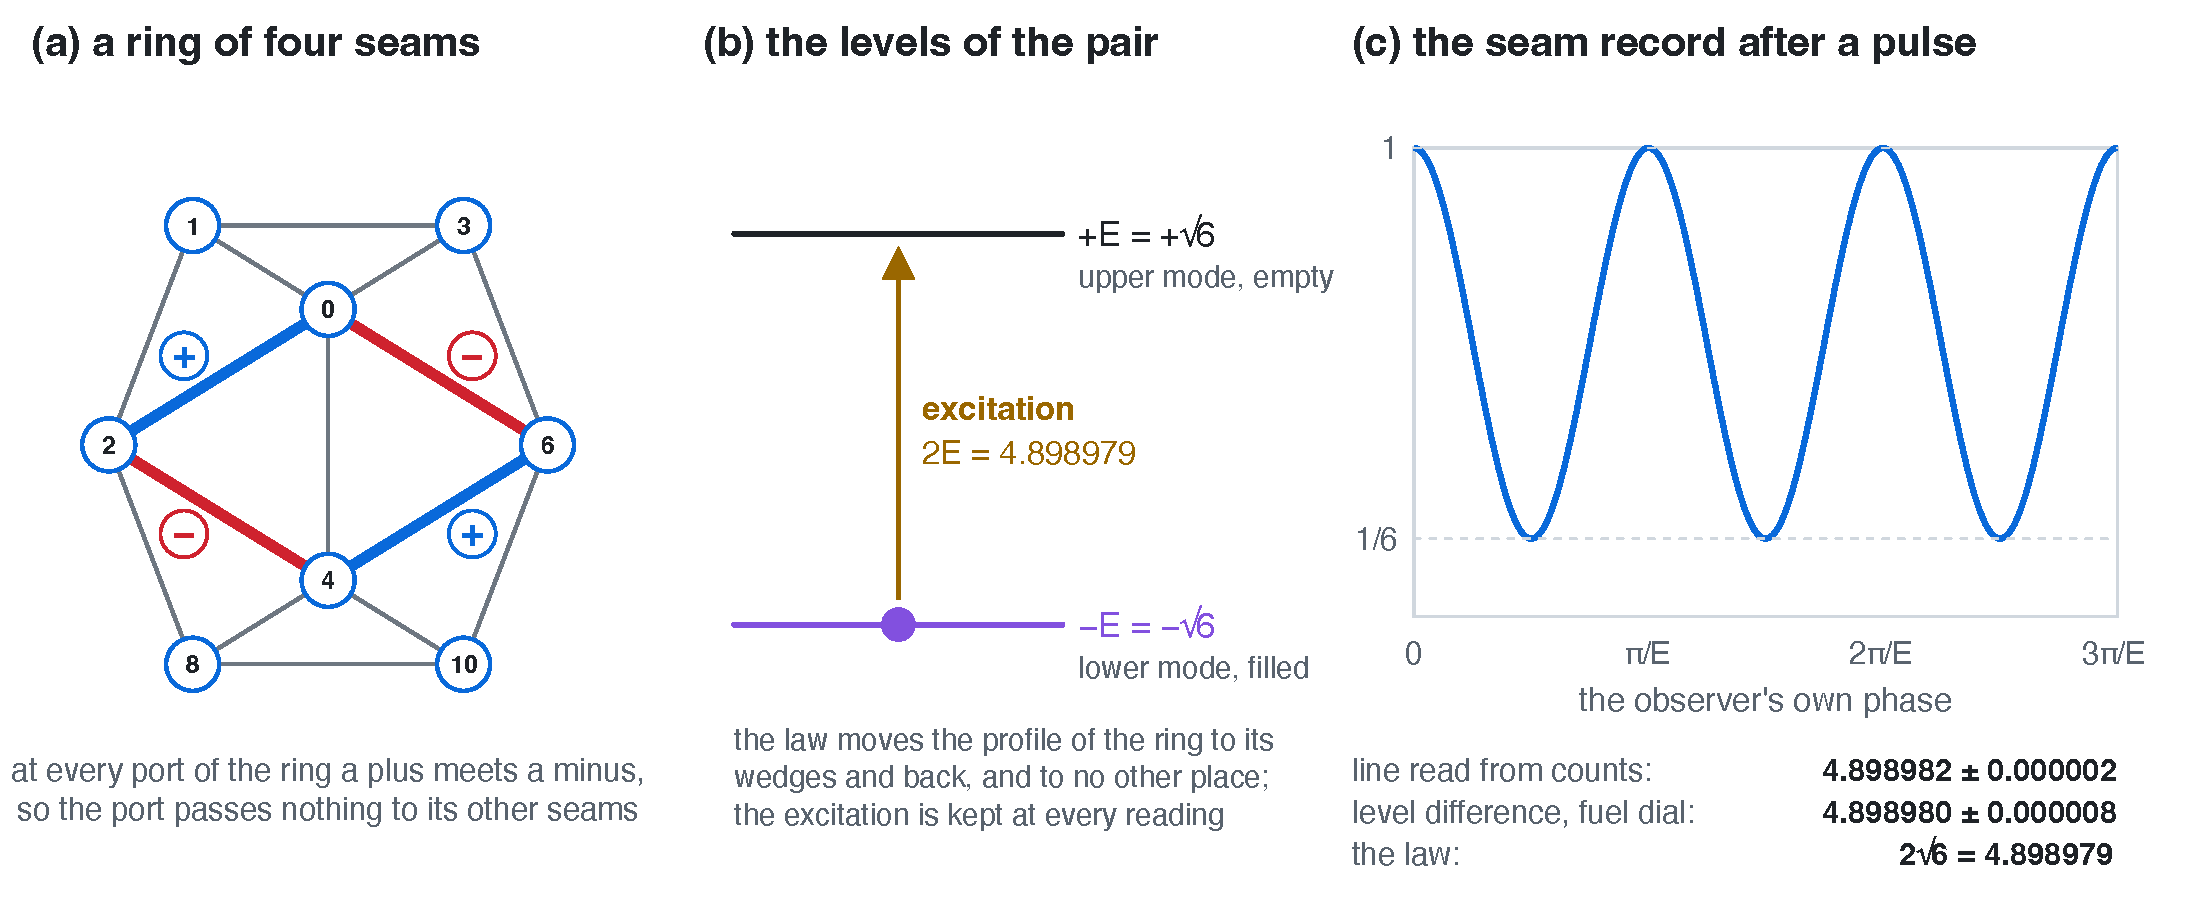
\includegraphics[width=\linewidth]{figures/model_cage.pdf}
\caption{The cage of the scalar channel. (a) A ring of four seams on one cell
with the signs $+,-,+,-$; at every port of the ring a plus meets a minus.
(b) The two levels $\pm E$ of the pair of the ring and the excitation that
lifts the object of the lower mode by $2E$. (c) The occupation of the profile
after the coherent pulse, $1-(\sigma^2/E^2)\sin^2(Et)$, against the
observer's own phase, with the line and the level difference read from
counts (Table~\ref{tab:cage}).}
\label{fig:cage}
\end{figure}

\subsection{What the observer of a cage reads}

The observer of a cage holds two operators on the profile: the number
$n(e)$ as a potential, and a converter between $e$ and a local fuel at
level zero. On the registers $n(e)=Q_e/8$ is a sum of $17$ words with
$Q_e^2=8Q_e$, and the converter is a sum of $8$ words. Both commute with all
$260$ loop conditions and touch the registers of the four ports of the
ring. The potential $-2E\,n(e)$ for the time
$\pi/\bigl(2\sqrt{2E(E-m)}\bigr)$ moves the object of the lower mode onto
$e$, and the potential $-(2E^2/m)\,n(e)$ for the time $\pi m/(2\sigma E)$
moves it into the upper mode. The observer's clock is the phase of a
circulation of three wedges at one of its ports, which sits at the level
$-m$ exactly; the observer reads that phase through its fuel with four
phase settings and states every frequency in units of this reference.

Three experiments are executed on one cell with the law running through
every step. In the first, the coherent pulse is followed by a wait of $q$
steps, and one trial reads the observer's reference and then, with the fuel
used as found, the occupation of the profile. In the second, a fuel whose
level is set by a dial is coupled weakly to the profile, with the fuel
prepared full and prepared empty; the difference of the two runs is the
survival of one object in the fuel, whatever the state of the pair is, and
the fuel empties where the dial meets a level of the pair. In the third, one
of three preparations is followed by a wait of $0$, $8$, $32$, $128$ or
$512$ steps and by one of four analyzers; the four counts give the
occupation matrix of the pair and from it the probability of the
excitation. Every reading is computed from sampled counts, $10^{8}$ trials
for each setting of the first and third experiment
(Table~\ref{tab:cage}).

\begin{table}[!htb]
\centering
\caption{Readings on a cage of one cell, from counts. Frequencies are in
units of the observer's own reference.}
\label{tab:cage}
\begin{tabular}{@{}L{8.3cm}L{3.4cm}r@{}}
\toprule
Reading & From counts & The law \\
\midrule
line of the seam record, steps of equal length & $4.898982\pm0.000002$ & $2\sqrt6=4.898979$ \\
the same line, steps of unequal length & $4.898976\pm0.000002$ & $4.898979$ \\
level difference of the pair, from the fuel dial & $4.898980\pm0.000008$ & $4.898979$ \\
amplitude of the line; with no pulse & $0.4161$; $0.0019$ & \\
excitation at five waits after the sharp pulse & $0.9999$ to $1.0002$ & $0.999954$ \\
excitation at five waits after the coherent pulse & $0.7059$ to $0.7060$ & $0.705932$ \\
excitation at five waits with no pulse & $0.000004$ & $0.000004$ \\
changed law: share of the variance in its best single line & $0.507$ & \\
changed law: largest distance of its counts from the record law of the law & $0.555$ & \\
\bottomrule
\end{tabular}
\end{table}

The values of the last column for the excitation are computed in the
prepared reference, which is why they differ from $1$ and from
$(1+m/E)/2=0.704$. An estimate from counts is linear in the counts and may
leave the range of a probability by its sampling error. With the two modes
of the cage stopped during the wait while the reference runs, the amplitude
of the line is below $10^{-5}$, and with the converter switched off no
record of a full fuel occurs. The changed law adds seam hopping round every
port, with the coefficient one, in every step of a run. It keeps the
alphabet, the routing, the number of objects and the symmetries of the
cell, and the observer's reference keeps its level under it. It does not
keep the pair: the lower mode holds $0.79$, $0.29$, $0.21$ and $0.14$ of
its weight in the pair at the parameter values $1$, $4$, $16$ and $64$.

\subsection{What the cage establishes}

Particle stability holds for a second object: the excitation of a cage is
kept for every interval by Theorem~\ref{thm:cage}, a local detector reads
it, and a changed law with the same alphabet, routing and symmetry loses
it. The cage carries a prepared clock: after a finite pulse its seam record
swings with no drive at one line, which the observer reads in units of its
own reference and finds equal to the level difference read separately. The
equality is the frequency condition of two levels, and it holds for every
$m$ and $c$. The pulse supplies the phase and the work of the swing, $E+m$
on the ideal reference. The reference by itself has a constant seam
record, and so has a sharp excitation. The observer takes as given that its
reference advances by between $1/16$ and $1/4$ in every step, since counts
cannot show a missed full turn. The level of a cage is flat: a cage has no
group speed, and the law holds no term between two objects.


\section{Where the outputs of the model meet the finite theorems}
\label{sec:joins}

The theory is a library of finite theorems, each proved under stated
premises and many of them machine-checked in Lean \cite{ophrepo}. The model
produces records. A theorem applies to the model where an output of the
model has the form of its premise, and its conclusion is then a statement
about the model's observers. The list below gives the theorems for which
this holds. Every entry is a statement about records: the state of the
simulation contains no spacetime, and no entry compares that state with the
world.

\begin{description}[leftmargin=1.2em,itemsep=3pt]
\item[The carrier.] \emph{Theorem:} the Gram matrix $G$ of the twelve port
directions has rank three and $G^2=4G$, and $G/4$ is the projector on the
band $5-\sqrt5$ of the port Laplacian $L$; machine-checked in
\path{Lean/Screen/PortFrameGram.lean} and
\path{Lean/Screen/PortGramRepairBand.lean} \cite{ophmicro}. \emph{The model
supplies} the cell, which is that table, and a law under which one load
moves with $L/2$ (Section~\ref{sec:loads}). \emph{It follows} that the
slowest motion of a load has exactly three independent directions, the
range of $G$. The first four levels of the scalar channel are the same
levels (Section~\ref{sec:scalar}).

\item[The seam rule.] \emph{Theorem:} four requirements leave one seam
rule: keep the total, end where $n_a^2+n_b^2$ is smallest, break a tie by a
coin that does not look at the loads, treat the two ports alike
\cite{ophmicro}; the rule leaves a difference $g$ of at most one and
lowers $n_a^2+n_b^2$ by $\tfrac12\bigl[(n_a-n_b)^2-g^2\bigr]$
(\path{Lean/ObserverPatchHolography/DirectedSeamRepair.lean}). \emph{The
model supplies} the write $W$ of Section~\ref{sec:local}, which is that
rule with the coin in superposition. \emph{It follows} that the event
which every seam writes and unwrites is the one rule with those
properties, and that its classical moves settle after a number of steps
that is polynomial in the number of ports for bounded loads. The echo
unwrites the event and conserves the multiset of loads, so this bound is a
statement about the moves and no statement about the law.

\item[The projective instrument.] \emph{Theorem:} a Kraus map with effect
$P$ that leaves every state certain for $P$ unchanged is the map
$X\mapsto PXP$, and conversely
(\path{Lean/EventAlgebra/InstrumentSelectionByCertainStates.lean}).
\emph{The model supplies} the presence reading of
Section~\ref{sec:presence}: it has the effect $P$ and leaves every state on
one answer block unchanged, on the ideal circuit and up to the known
diagonal phase of the read window. \emph{It follows} that the presence
reading is the projective instrument of the event ``a pair on some seam''.
The reader with its seam hidden has the same effect and fails the
condition on the uniform superposition of the thirty pairs, so by the
converse it is another instrument. That is the difference between the two
histories of Table~\ref{tab:presence}.

\item[Records.] \emph{Theorem:} orthogonal record projectors generate a
commutative algebra with Born weights and L\"uders conditioning, an
immediate reread returns the record with probability one
\cite{ophconsensus}, and two different states that one isometry copies
from the same blank are orthogonal
(\path{Lean/EventAlgebra/NoBroadcastingAdapter.lean}). \emph{The
model supplies} readers with complete outcome sets that copy orthogonal
labels, public records that the law never erases, and a seam label that no
event changes. \emph{It follows} that the agreed records of the model form
a public algebra with certain rereads, and that a reading which keeps one
answer for the cell has to unwrite the seam words, as the presence reading
does.

A scheduled publication circuit also delivers a single measured
word to every owner on the 20-, 80- and 320-cell boards. Each parent
reads its own stored rails, writes its outgoing register and transfers
it through native contacts to a child. The empty receiving register
and a delivered source refusal have distinct readings. On the
320-cell board every owner matched the source in 65,536 simulated
launches. Replacing the last reader's word with an independent local
sample preserved its theoretical outcome frequencies and disagreed on
40,980 individual launches. The two records agree with probability
$3/8$ under independent resampling. Every delivered word preserved its
correlation with the second bit read on the source dimer. For the
ideal copying step applied after the label is recorded, a partial trace
preserves arbitrary reference correlations within each label block
(\path{model/experiments/interval_echo_consensus/publication_tree/}).

A single native balancing write can itself produce two public readings.
On 20, 80 and 320 cells, both gateway owners read half the incoming
load sum whenever it was even. At odd sums both readers have the same
single-site distribution, yet their adjacent readings differed on every
launch. Tracing the coin, signed head and opposite endpoint removes
every off-diagonal incoming matrix unit. Among all 511 nonempty sharp
input supports, seven allow three exactly recoverable local answers,
111 allow two and 393 allow one. After opening an additional neighboring
contact, the inputs $(1,1)$ and $(0,2)$ that had both announced one
gave respectively 65,536 and 32 disagreements in 65,536 starts at the
half-turn appointment. The earlier number is public at the writing
event; its later availability depends on the material continuation
(\path{publication_tree/repair_outputs/}).

A collective of twelve separately named readers implements the
finite capacity packet's authorized set. On each of the three board
sizes, each station reads one local bit. One exceptional high or low
bit among twelve identifies the port and orientation. The joint read
recovers all 24 records under each of 40 reported continuation settings.
Every eleven-reader subset separates all 24. A particular ten-reader
subset gives 22 distinct profiles at identity, but the largest common
code recoverable with \emph{any} ten readers has only two words:
a ten-reader group can miss the two sites distinguishing any pair of
the same orientation. After twelve rounds of physical communication on
the small board, individual stations recovered all 288 held records.
Omitting one handoff produced 168 refusals. The original publicness
rule always requests all twelve positions. Its code size describes this
prepared alphabet (\path{publication_tree/authorized_sets/}).

\item[Local operations.] \emph{Theorem:} a complete operation on one
factor of a product leaves the reduced state of every other factor
unchanged \cite{ophconsensus}. \emph{The model supplies} seam events and
seam readings that act on the registers of one seam. \emph{It follows} that
no event or reading changes the record law of an observer that shares no
register with it.

\item[The generator.] \emph{Theorem:} a continuous one-parameter group of
automorphisms of a finite matrix block is conjugation by $e^{-itH}$, with
$H$ unique up to an additive constant \cite{ophobservers}. \emph{The model
supplies} two such flows, the free evolution of the contrast-memory seam,
which Interval Echo uses at $\kappa=8$, and that of the scalar channel.
\emph{It follows} that each free evolution is fixed by its flow up to an
energy offset. The parameter $t$ is no observer's clock.

\item[Frequencies.] \emph{Theorem:} a reading that intertwines the
frequencies of its source with its own shows no frequency that the source
lacks (\path{Lean/QFT/ModularClockComparison.lean}). \emph{The model
supplies} the pair of a cage, whose frequencies are $0$ and $\pm2E$
(Theorem~\ref{thm:cage}). \emph{It follows} that a record of the pair
under the free law holds the one line $2E$, which the observer reads from
counts at $4.8990$ of its reference (Table~\ref{tab:cage}).

\item[Clocks.] \emph{Theorem:} two shared readings fix the positive affine
map between two clocks, and it is unique (\path{Lean/Time/ClockReadout.lean}).
\emph{The model supplies} ports that count their own events and share the
records of their seams, and under Interval Echo two observer patches that
read both elapsed counts on one common seam at reunion
(Section~\ref{sec:echo}). \emph{It follows} that two shared records relate
the counts of two observers and a third checks the relation. No common
clock enters.

\item[Rereads.] \emph{Theorem:} for a state in the range of an event
projector, $n$ rereads of the event over a total parameter $t$ all return
it with probability at least $1-2t^2\lVert H\rVert^2/n$
\cite{ophobservers}. \emph{The model supplies} the presence reading and
the law. \emph{It follows} that frequent presence readings would hold a
pair at any coupling. Every reading of Section~\ref{sec:stability}
therefore uses a fresh run, and the binding theorem needs no reading.

\item[The port response.] \emph{Theorem:} a faithful closed
twelve-dimensional response with a positive trace form, on which the
carrier rotations act by inner automorphisms, has the Lie type
$\mathfrak u(1)\oplus\mathfrak{su}(2)\oplus\mathfrak{su}(3)$ \cite{ophgauge}. \emph{The model supplies}
the response of one load on one cell under the declared service of
Section~\ref{sec:response}. \emph{It follows} that this response has that
type, and the direct computation gives $\mathfrak u(3)\oplus\mathfrak{so}(3)$,
the same type.
Under the plain services the response has seventeen directions and the
premise fails. Interval Echo supplies twelve independent port currents
selected by the rotations, on one load and on the bound pair, closed under
commutators and covariant under the rotations (Section~\ref{sec:echo});
that this menu is complete for a physical observer is not established.
\end{description}

\paragraph{Theorems that consume other outputs.}
Other finite theorems of the theory consume outputs that the model does not
produce in the required form. The settling theorems of the consensus paper
consume accepted repairs that lower a well-founded measure and close every
fork \cite{ophconsensus}. The free evolutions of the model are unitary and
conserve their loads and objects, so for them those theorems apply to the
classical seam rule and make no statement about the echo. In the repair
experiment of Interval Echo on one cell a seam write is accepted when a
sharp reading finds both ends holding one load, and each accepted write
lowers the sum of the squared loads. Two such repairs competing for one
doubled load leave distinguishable records; a prepared local priority,
read without being moved, makes both request orders end in one common
terminal state in all six combinations of sharp preparation and priority.
No confluence of all accepted repairs on the federation is proved. The
proposition on smooth effective
field descriptions consumes readouts that are polynomials in the Weyl
operators of a free field on a radial cylinder over the screen
\cite{ophspacetime}; the readouts of the model are instruments on finite
registers. The causal and count limits consume an authenticated order of
events with its placement and a refinement family. The matched-regional
Einstein theorem consumes entropy, area and stress readouts of one region
in a common frame. The Maxwell selection theorems consume a gauge-invariant
action on seam potentials, and the theorems on defect classes and
statistics a five-level code with a spin doublet. The dark-sector theorems
consume a modular generator with a recovery defect, where the unrecovered
collar supplies a conserved label \cite{ophdarkmatter}. Each of these names
an output that a member of the model has to produce before the theorem
applies to it.


\section{Resources and the scope of the computations}
\label{sec:resources}

A literal allocation of the reference candidate on the federation of $20$
cells has $240$ load systems of three states, $630$ seam memories of eleven
states, $180$
reference registers of three states with $180$ further memories of eleven
states for the degree term, one fuel system of two states and $630$ reader
blocks of eleven bits. Its dimension is
\[
3^{240}\cdot11^{630}\cdot(3\cdot11)^{180}\cdot2\cdot2^{11\cdot630},
\]
about $10{,}399$ bits. The computations of this paper use sectors of this
space that the law maps into themselves. By Corollary~\ref{cor:network} the
memories stay blank, and the sector of two loads has $V(V+1)/2$ states on
$V$ ports (Table~\ref{tab:carriers}); the unit pairs form an invariant part
of it, and the emitter adds one state. The sector of three unit loads has
$220$ states on one cell and $2{,}275{,}280$ on $20$ cells. The complete
reading of Section~\ref{sec:instruments} has $161{,}792$ states. These
sizes are polynomial in the number of ports because the number of loads is
fixed. The space of many loads, and the allocation above, grow
exponentially with the number of ports.

The statements for every federation, Theorem~\ref{thm:binding},
Corollary~\ref{cor:emitted} and Proposition~\ref{prop:reader}, are operator
estimates and no claim that the allocation of a whole federation with its
readers was propagated.

The construction encodes no constraint
instance, decodes no witness from its records and reaches no fixed point,
since the law conserves the multiset of loads. It is no solver for general
constraint problems and claims no polynomial bound for one.


\section{Supplied parts and limits of the construction}
\label{sec:scope}

\subsection{Supplied}

The following parts are design choices of the construction.
\begin{itemize}[leftmargin=1.6em,itemsep=1pt]
\item The coupling $\kappa$. Computed values are $0$, $0.5$, $1$, $2$, $4$,
$8$, $16$, $64$ and $128$, with $8$ and $128$ in the main tables.
\item The coherent generator $M_\kappa$ on the private seam memory, and the
blank initial state of every memory.
\item The reference registers of the degree term on ports with five seams.
\item The emitter with its fuel, coupling and duration, the timing of the
reader, and the public record as a protected memory.
\item The evolution parameter of the runs with a continuous parameter. As
local events the pair needs every seam to act once per round, or the limit
of small angle, and the event programs use the event \eqref{eq:event}
(Section~\ref{sec:events}).
\item The routing of the federation by the cell-centre and tangent-frame
convention.
\item The weighted port service \eqref{eq:service} of
Section~\ref{sec:response}, and the unrecovered collar with its fuel and
converter in Section~\ref{sec:collar}.
\item The tree of the presence reading with its wiring and pulse schedule
(Section~\ref{sec:presence}).
\item For the scalar channel: its two coefficients $m$ and $c$, the
prepared reference with its ramps, the apparatus registers and the
penalties of the register form, the two operators on a profile, the pulses
with their strengths and times, the fuel dial, and the bounds on a step of
the observer's reference (Section~\ref{sec:scalar}).
\item For Interval Echo: the guide, custody transfers, gate selection,
relative cadence and read windows of the clock, the prepared hands, the
designed sizes of the hand, the two counts and the walk budget, and the
calibrated closing filter; the preparations, matching schedule, tag
protection and gate windows of the overlap measurements; and the oriented
cell, preparation, protected bands and unit gain of the port-current
service (Section~\ref{sec:echo}).
\end{itemize}

\subsection{Limits}

The construction does not supply the following.
\begin{itemize}[leftmargin=1.6em,itemsep=1pt]
\item A selection of $\kappa$. The collar reading of
Section~\ref{sec:collar} returns the coupling from records; no equation
fixes its value.
\item A particle--antiparticle assignment in the contrast-memory law.
One load per port supports an excess and a vacancy, but their free
evolution conserves both counts. In the scalar channel an object above the
filled reference and a missing object below it are the two signs, and the
law holds no term between two objects.
\item A physical electromagnetic connection. In the written-field
extension of Section~\ref{sec:written-signed-load}, head changes carry
signed flux and a distant material probe responds. A static Coulomb
interaction and a transverse Maxwell branch have no realization in
the tested ground and ordered channel, respectively.
\item The class of an object as a record. Objects are protected by the
number of loads and the gap alone (Section~\ref{sec:objects}).
\item The twelve port currents on the bound object from the reference
law's own services (Section~\ref{sec:response}). Interval Echo obtains
twelve from a supplied service selected by the rotations, and a complete
menu of the physical controls is not identified (Section~\ref{sec:echo}).
\item One limiting speed for all objects. The bound pair is a Galilean
composite: on a chain, with the seam term \eqref{eq:xxz}, one load has the
branch $\Delta-\cos k$ and the pair has
$E(K)=\Delta-\cos^{2}(K/2)/\Delta$ with $\Delta=1+2\kappa$, which is
quadratic at small $K$. At $\kappa=8$ the kinetic ratios of free clusters
differ from their rest-energy ratios, so under the free law, which
Interval Echo inherits, rest energy and inertia of free clusters follow two
dictionaries. The scalar channel has the relation
$\omega^2=m^2+\lambda$ by the form of its law, and its cage has a flat
level and does not move.
\item A clock that starts with no supplied phase. The swing of a cage is
written by a pulse that supplies its phase and its work.
\item A refinement map that preserves seams. The port-ancestry map between
the levels of the federation does not preserve seam adjacency
\cite{ophmicro}. The test of a refinement is agreement of the distributions
of admissible observer records between levels; agreement of state encodings
is no part of it.
\item A comparison of clocks on held clock constructions and directions.
The clocks of Section~\ref{sec:events} are counts of events, and the patch
clock of Interval Echo follows the relativistic proper-time forecast on the
journeys of Section~\ref{sec:echo}.
\item The transport of the three directions by a moving observer's full
records.
\item The regional response that the Einstein theorem of the spacetime
paper consumes \cite{ophspacetime}.
\item A physical reading of the unrecovered collar as the dark-sector
carrier of the theory (Section~\ref{sec:collar}).
\end{itemize}

These limits are measured against the test of Section~\ref{sec:intro}.
Observers who inhabit the computation can describe their experience as a
relativistic continuum spacetime with one time and three space dimensions,
by the proposition on smooth effective field descriptions of the flagship
and the reconstruction of the spacetime paper, under their stated premises
\cite{flagship,ophspacetime}. Of those premises the model supplies the
carrier with its rank-three band, count clocks compared through shared
readings (Section~\ref{sec:joins}) and, under Interval Echo, clocks carried
by observer patches that run slow by the relativistic factor when they move
(Section~\ref{sec:echo}); the field readouts, a jointly authenticated order
of events and the refinement family that the two results also consume are
outputs it does not produce. The model is not required to contain three
dimensions in its state, and no item above asks for that.


\section{What the model predicts on records}
\label{sec:predictions}

Every result of this paper is a probability of records under a stated
preparation. Each is therefore a prediction for any realization of the
model, on a quantum processor or in an independent simulation: the
realization prepares, runs and reads as specified and compares its counts
with the numbers of Table~\ref{tab:predictions}. The table names for each
prediction the outcome that counts against it. These are predictions about
the model. A comparison with a laboratory system requires in addition that
the same preparation, intervention and readout be identified in that
system.

\begin{table}[!htb]
\centering\small
\caption{Predictions of the model on records, and the outcome that counts
against each.}
\label{tab:predictions}
\begin{tabular}{@{}L{4.6cm}L{6.3cm}L{4.4cm}@{}}
\toprule
Experiment & Prediction & Counts against it \\
\midrule
A pair written on one seam, read later, $\kappa>3$ & no pair with probability at most $40/(2\kappa-6)^2$ on every federation; at most $0.0097$ at $\kappa=8$ on $1$ to $320$ cells & a larger probability at some reading \\
The same law without the agreement energy & no pair with probability up to $0.80$ on $20$ cells & a pair that is kept \\
Rounds of seam events in any order, with unequal rates of the ports & the pair is kept & a loss of the pair under rounds \\
Two readings of a pair, $\kappa=8$, one cell & equal first answers; later records that differ by more than $0.0817$ in total variation; one event at $0.0183$ against $0.1029$ & equal laws of the later records \\
An unrecovered collar with empty ports & read unrecovered at every reading; the rates of its two records return the coupling & a recovery; another ratio of the rates \\
The seam record of a cage after the coherent pulse & one line at $2\sqrt6=4.8990$ of the observer's reference, with more than $0.9999$ of the variance & a second line, or a line elsewhere \\
The fuel dial on the same cage & the level difference $4.8990$, equal to the line & a value away from the line \\
The excitation of a cage after the sharp pulse & read above $0.99$ at waits of $0$ to $512$ steps, the same at every wait & a decrease with the wait \\
The cage under seam hopping round every port & no single line; the excitation is lost & a single line, or a kept excitation \\
Interval Echo: a travelling patch on journeys with leg speeds $(1/2,1/6)$, $(1/6,1/2)$ and $(1/4,1/4)$ & a ratio of its elapsed count to the home count at reunion within about $0.001$ of the forecast \eqref{eq:echo-forecast} & a residual far outside its standard error \\
Interval Echo: overlapping single-cell and three-cell observers on $320$ cells & equal readings at every shared checkpoint & a shared checkpoint read differently \\
\bottomrule
\end{tabular}
\end{table}


\section{Conclusion}
\label{sec:conclusion}

The reference candidate A-contrast-memory-spherical-v1 is a finite
specification with every part stated: a carrier of icosahedral cells,
loads on ports, a private memory
on every seam, one local term for each seam, an emitter, a reader with a
complete outcome set, and the schedules under which the law is run. The
echo with the contrast-memory generator is exactly the exchange with an
energy of agreement, and the written output enters through its symmetry
alone. The law binds a pair of loads with constants that hold for every
number of cells, the agreed records show the pair on changing seams, and
the law without the agreement energy loses it. The same law has bound
objects on seams and faces, a port response of seventeen directions that
becomes twelve under one declared service, and a conserved neutral
excitation of the seam memory. Two readings of the pair, one that keeps a
single answer for the cell and one that keeps the seam, have the same first
statistics and different later records. The main candidate law, Interval
Echo, runs this seam at $\kappa=8$ and lets a finite observer patch carry
its own clock. A travelling clock, compared at reunion with the clock kept
at home, runs slow by the relativistic factor computed from the observers'
own records, within about one part in a thousand. Overlapping observers
agree on every shared checkpoint reading, port currents selected by the
rotations close on twelve directions, and two overlapping observers realize
the unique information projection to a uniform reference. The second
candidate law on the same carrier holds an object on four seams by the
signs of its hop: its excitation is kept for every interval, and its seam
record carries a prepared clock that an observer reads in units of its own
reference. All three laws are candidate native repair laws, and their
couplings are supplied.

The written-field extension identifies a candidate for the charge and
field response of an electron. Its signed material load carries the
change in boundary flux, alters a distant material probe and responds
to an orbital magnetic twist. The four-face field doublet changes how
that charge moves, yet an addressed exchange carries the material
origins past one another while leaving the doublet labels at their
original gateways. Physical spin attached to the travelling charge,
fermionic exchange of the whole excitation and its rest energy in keV
are distinct, unverified identifications. On the original Interval Echo
law the long-wave dispersion measured on a prepared four-port route
depends on how the same gateways are connected inside each cell
(Section~\ref{sec:written-route}).


\section{Reproducibility}
\label{sec:repro}

The reference candidate is the package
\path{model/candidate_laws/contrast_memory_spherical_v1} of the public
repository \cite{ophrepo}. The command
\begin{center}
\texttt{python -m model.candidate\_laws.contrast\_memory\_spherical\_v1.verify}
\end{center}
recomputes the reference candidate from the carrier arrays of the package
and compares
the outcome with the stored results; with the option \texttt{-{}-full} it
also recomputes the federations of $80$ and $320$ cells and the event
programs. It checks the identities of Section~\ref{sec:local} in exact
arithmetic on all $99$ local states, counts the incidence facts of
Lemma~\ref{lem:incidence} on the federations, computes the constants of
Table~\ref{tab:constants}, and recomputes the record probabilities of
Sections~\ref{sec:instruments}, \ref{sec:events} and~\ref{sec:stability},
the objects and bindings of Section~\ref{sec:objects}, the port response of
Section~\ref{sec:response} and the collar levels and readings of
Section~\ref{sec:collar}. Exact identities must hold exactly, and floating
values are compared within declared tolerances. Sampled readings use fixed
seeds. The proofs of Sections~\ref{sec:carrier} to~\ref{sec:events} are
given in full in the text and do not depend on the computations.

The commands
\begin{center}
\texttt{python -m model.candidate\_laws.contrast\_memory\_spherical\_v1.presence}\\
\texttt{python -m model.candidate\_laws.contrast\_memory\_spherical\_v1.presence\_certificate}\\
\texttt{python -m model.candidate\_laws.scalar\_channel}\\
\texttt{python -m model.experiments.cage}
\end{center}
recompute the laws of two readings of Section~\ref{sec:presence}, the
certified event in exact arithmetic, the scalar channel of
Section~\ref{sec:scalar} and its cage. The counts of the experiments
on a cage are stored with the package. A replay recomputes the record laws
from the law and the prepared reference, checks that the stored counts are
draws from them, and recomputes every reading from the counts.

The command
\begin{center}
\texttt{python -m model -{}-full}
\end{center}
replays the main candidate law, Interval Echo, and compares the outcome
with the stored results: the material clock transfers on $20$, $80$ and
$320$ cells, the reunion cohorts, the overlap measurements, the repair
fork, the port currents and the information projection of
Section~\ref{sec:echo}. The journeys timed by light pulses are archived
with their mean records and standard errors, from which the reported
residuals follow.

The signed-load experiments of Section~\ref{sec:written-signed-load} are
documented in \path{model/candidate_laws/interval_echo/openwave/electron_field/}.
The route spectra and local frequency records of Section~\ref{sec:written-route}
are in \path{row_30_route/} and \path{row_30_autonomous/}.
The domain-wall measurements of Section~\ref{sec:collective-wall} are in
\path{row_30_collective/} and \path{submission/row_30_cautions/}. These packages are under
\path{model/candidate_laws/interval_echo/openwave/}.

% Generated by tools/build_prior_work.py from the claims ledger; do not edit.
\section*{Credited prior work}

The results of this paper build on the following established work. Each
entry names an established result as it is used here and cites its sources.

\begin{itemize}\setlength{\itemsep}{0pt}
\item Algebraic graph theory and symmetric spectral methods~\cite{pwbiggs1993algebraic,pwparlett1998symmetric}.
\item Finite-dimensional states, quantum channels and partial traces~\cite{pwnielsen2010quantum}.
\end{itemize}


\section*{Statements and declarations}

\noindent\textbf{Funding.}
The authors declare that no external grants or dedicated third-party research
funding were received for the preparation of this manuscript.

\noindent\textbf{Competing interests.}
The authors participate in OPH-related research, software, simulation, or
prototype-development programs and may receive professional or reputational
benefit from this work. These relationships are disclosed. The authors declare
no other competing interests.

\noindent\textbf{Data availability.}
The model documents, executable sources and computed results supporting this
study are available in the public OPH repository \cite{ophrepo}.

\noindent\textbf{Corresponding author.}
Correspondence should be addressed to Bernhard Mueller,
\href{mailto:bernhard@floatingpragma.ai}{\nolinkurl{bernhard@floatingpragma.ai}}.

{\footnotesize
\begin{thebibliography}{99}

\bibitem{hofmannreturns}
H.~F. Hofmann, Complementary classical fidelities as an efficient criterion
for the evaluation of experimentally realized quantum operations,
\emph{Physical Review Letters} \textbf{94}, 160504 (2005),
\href{https://doi.org/10.1103/PhysRevLett.94.160504}{doi:10.1103/PhysRevLett.94.160504}.

\setlength{\itemsep}{0pt}\setlength{\parsep}{0pt}

\bibitem{ophrepo}
FloatingPragma (2026). \emph{Observer Patch Holography}: papers, Lean library,
executable model, receipts and claim registries. Public repository; model
documents, receipts, papers and the basis document are cited at the release
tag of this paper, and frozen custody records at their registration
revisions.
\url{https://github.com/FloatingPragma/observer-patch-holography/tree/r2073}

\bibitem{flagship}
Mueller, B., Poneder, M., Osika, A., Xue, K., Cassie, B., Nguyen, P., Kim, J.,
Matscheko, D., Friedman, D.\,A., Hill, J., Glynn, W.\,T., Visser, M.\,A., Anirudha, K.\,A., and de La Fourni\`ere, B. (2026). \emph{Observers Who Read Their Universe into Existence: Finite Consensus and the Reconstruction of Standard Physics}. Public manuscript.
\url{https://github.com/FloatingPragma/observer-patch-holography/blob/r2073/flagship/from_observer_consensus_to_standard_physics.pdf}

\bibitem{ophobservers}
Mueller, B., Poneder, M., Osika, A., Xue, K., Cassie, B., Nguyen, P., and Friedman, D.\,A.
(2026). \emph{Observers Are All You Need}. Public manuscript.
\url{https://github.com/FloatingPragma/observer-patch-holography/blob/r2073/paper/observers_are_all_you_need.pdf}

\bibitem{ophgauge}
Mueller, B., Poneder, M., Osika, A., Xue, K., Nguyen, P., Matscheko, D., and Friedman, D.\,A.
(2026). \emph{Standard Model Gauge Structure under Complete-Response and Observer-Transport Premises}. Public manuscript.
\url{https://github.com/FloatingPragma/observer-patch-holography/blob/r2073/paper/deriving_standard_model_gauge_structure_from_observer_overlap_consistency.pdf}

\bibitem{ophspacetime}
Mueller, B., Poneder, M., Osika, A., Xue, K., Nguyen, P., Visser, M.\,A.,
Matscheko, D., and de La Fourni\`ere, B. (2026). \emph{Recovering Observer
Spacetime and Einstein Dynamics from Overlap Consistency}. Public manuscript.
\url{https://github.com/FloatingPragma/observer-patch-holography/blob/r2073/paper/recovering_observer_spacetime_and_einstein_dynamics_from_overlap_consistency.pdf}

\bibitem{ophconsensus}
Mueller, B., Xue, K., Kim, J., Anirudha, K.\,A., Matscheko, D., and Hill, J.
(2026). \emph{Reality as a Consensus Protocol: The Fixed-Point Computation
That Implements Physics}. Public manuscript.
\url{https://github.com/FloatingPragma/observer-patch-holography/blob/r2073/paper/reality_as_consensus_protocol.pdf}

\bibitem{ophmicro}
Mueller, B., Osika, A., Xue, K., Cassie, B., de La Fourni\`ere, B., and Friedman, D.\,A. (2026).
\emph{Twelve-Port Icosahedral Carriers and Native Seam Repair: The Carrier Layer of Observer Patch Holography}. Public manuscript.
\url{https://github.com/FloatingPragma/observer-patch-holography/blob/r2073/paper/screen_microphysics_and_observer_synchronization.pdf}

\bibitem{ophdarkmatter}
Mueller, B., and Matscheko, D. (2026). \emph{Observer Patch Holography and the
Dark Sector: Modular Charge, the Anomalous Collar Source, and the Deep Galaxy
Law}. Public manuscript.
\url{https://github.com/FloatingPragma/observer-patch-holography/blob/r2073/cosmology/oph_dark_matter_paper.pdf}

\bibitem{nachtergaele2001}
Nachtergaele, B., and Starr, S. (2001). ``Droplet states in the XXZ
Heisenberg chain.'' \emph{Communications in Mathematical Physics}
\textbf{218}, 569--607. \url{https://arxiv.org/abs/math-ph/0009002}

\bibitem{fischbacher2018}
Fischbacher, C., and Stolz, G. (2018). ``Droplet states in quantum XXZ spin
systems on general graphs.'' \emph{Journal of Mathematical Physics}
\textbf{59}, 051901. \url{https://arxiv.org/abs/1712.10276}

\bibitem{daviskahan1970}
Davis, C., and Kahan, W.\,M. (1970). ``The rotation of eigenvectors by a
perturbation. III.'' \emph{SIAM Journal on Numerical Analysis} \textbf{7}(1),
1--46. \url{https://doi.org/10.1137/0707001}

\bibitem{bhatia1997}
Bhatia, R., and Rosenthal, P. (1997). ``How and why to solve the operator
equation $AX-XB=Y$.'' \emph{Bulletin of the London Mathematical Society}
\textbf{29}(1), 1--21. \url{https://doi.org/10.1112/S0024609396001828}

\bibitem{strang1968}
Strang, G. (1968). ``On the construction and comparison of difference
schemes.'' \emph{SIAM Journal on Numerical Analysis} \textbf{5}(3), 506--517.
\url{https://doi.org/10.1137/0705041}

\bibitem{pdgleptons2026}
F.~Takahashi et al. (Particle Data Group), \emph{Int. J. Mod. Phys. A}
\textbf{41}, 2630011 (2026), lepton summary, pp.~1--2.
\url{https://pdg.lbl.gov/2026/tables/rpp2026-sum-leptons.pdf}

\bibitem{codata2022ratio}
P.~J. Mohr et al., \emph{Rev. Mod. Phys.} \textbf{97}, 025002 (2025),
Eq.~(187). \url{https://doi.org/10.1103/RevModPhys.97.025002}

\bibitem{farnham}
D.~L. Farnham, R.~S. Van Dyck, Jr., and P.~B. Schwinberg,
\emph{Phys.\ Rev.\ Lett.} \textbf{75}, 3598 (1995).
\url{https://doi.org/10.1103/PhysRevLett.75.3598}

\bibitem{rainville}
S. Rainville et al., \emph{Hyperfine Interactions} \textbf{132},
177--187 (2001), Table~I.
\url{https://doi.org/10.1023/A:1011922529114}

\bibitem{bouchendira}
R. Bouchendira et al., \emph{Phys.\ Rev.\ Lett.} \textbf{106}, 080801
(2011). \url{https://doi.org/10.1103/PhysRevLett.106.080801}

% Generated by tools/build_prior_work.py from the claims ledger; do not edit.
\bibitem{pwbiggs1993algebraic}
Biggs, N. (1993). \emph{Algebraic Graph Theory}. Cambridge University Press. \url{https://doi.org/10.1017/CBO9780511608704}

\bibitem{pwnielsen2010quantum}
Nielsen, M. A., and Chuang, I. L. (2010). \emph{Quantum Computation and Quantum Information: 10th Anniversary Edition}. Cambridge University Press. \url{https://doi.org/10.1017/CBO9780511976667}

\bibitem{pwparlett1998symmetric}
Parlett, B. N. (1998). \emph{The Symmetric Eigenvalue Problem}. Society for Industrial and Applied Mathematics. \url{https://doi.org/10.1137/1.9781611971163}



\bibitem{branciard2012}
C.~Branciard, D.~Rosset, N.~Gisin and S.~Pironio,
Bilocal versus nonbilocal correlations in entanglement-swapping experiments,
\emph{Physical Review A} 85 (2012), 032119.
\href{https://doi.org/10.1103/PhysRevA.85.032119}{doi:10.1103/PhysRevA.85.032119}.

\bibitem{chsh1969}
J.~F. Clauser, M.~A. Horne, A.~Shimony and R.~A. Holt,
Proposed experiment to test local hidden-variable theories,
\emph{Physical Review Letters} 23 (1969), 880--884.
\href{https://doi.org/10.1103/PhysRevLett.23.880}{doi:10.1103/PhysRevLett.23.880}.

\end{thebibliography}}

\section*{AI Assistance Disclosure}
This research project used research-grade commercial models, including
Anthropic's Fable and OpenAI's GPT-6 Astra, for research support, software
development, editing, and synthesis. The authors are responsible for the
paper's claims, methods, and final text.

\end{document}
